% TODO:
% * 打开\makecover
% * 添加数组融合的图片
% * 把SC论文中其他部分添加进来(还有不少新内容)
%
\documentclass[degree=doctor]{thuthesis}
%\documentclass{ctexart}
% 选项:
%   degree=[bachelor|master|doctor|postdoctor], % 必选
%   secret,                                     % 可选
%   pifootnote,                                 % 可选(建议打开)
%   openany|openright,                          % 可选,基本不用
%   arial,                                      % 可选,基本不用
%   arialtoc,                                   % 可选,基本不用
%   arialtitle                                  % 可选,基本不用

% 所有其它可能用到的包都统一放到这里了,可以根据自己的实际添加或者删除。
\usepackage{thuthesis}
\usepackage{bm}
\usepackage{lscape}
\usepackage{algorithm}
\usepackage[noend]{algpseudocode}
\usepackage{silence}
\usepackage{multirow}
%\usepackage[normalem]{ulem}
%\useunder{\uline}{\ul}{}
\WarningFilter{latex}{Float too large}
% 定义所有的图片文件在 figures 子目录下
\graphicspath{{figures/}}

% 可以在这里修改配置文件中的定义。导言区可以使用中文。
% \def\myname{薛瑞尼}
\begin{document}

%%% 封面部分
%\frontmatter
%\thusetup{
  %******************************
  % 注意:
  %   1. 配置里面不要出现空行
  %   2. 不需要的配置信息可以删除
  %******************************
  %
  %=====
  % 秘级
  %=====
  secretlevel={秘密},
  secretyear={10},
  %
  %=========
  % 中文信息
  %=========
  ctitle={面向神威太湖之光的地震应用并行优化方法研究},
  cdegree={工学博士},
  cdepartment={计算机科学与技术系},
  cmajor={计算机科学与技术},
  cauthor={何聪辉},
  csupervisor={付昊桓副教授},
  %cassosupervisor={陈文光教授}, % 副指导老师
  %ccosupervisor={某某某教授}, % 联合指导老师
  % 日期自动使用当前时间,若需指定按如下方式修改:
  %cdate={2018年03月},
  %
  % 博士后专有部分
  % cfirstdiscipline={计算机科学与技术},
  % cseconddiscipline={系统结构},
  % postdoctordate={2009年7月——2011年7月},
  % id={编号}, % 可以留空: id={},
  % udc={UDC}, % 可以留空
  % catalognumber={分类号}, % 可以留空
  %
  %=========
  % 英文信息
  %=========
  etitle={Accelerating the Seismic Applications on Sunway TaihuLight Supercomputer},
  % 这块比较复杂,需要分情况讨论:
  % 1. 学术型硕士
  %    edegree:必须为Master of Arts或Master of Science(注意大小写)
  %             “哲学、文学、历史学、法学、教育学、艺术学门类,公共管理学科
  %              填写Master of Arts,其它填写Master of Science”
  %    emajor:“获得一级学科授权的学科填写一级学科名称,其它填写二级学科名称”
  % 2. 专业型硕士
  %    edegree:“填写专业学位英文名称全称”
  %    emajor:“工程硕士填写工程领域,其它专业学位不填写此项”
  % 3. 学术型博士
  %    edegree:Doctor of Philosophy(注意大小写)
  %    emajor:“获得一级学科授权的学科填写一级学科名称,其它填写二级学科名称”
  % 4. 专业型博士
  %    edegree:“填写专业学位英文名称全称”
  %    emajor:不填写此项
  edegree={Doctor of Philosophy},
  emajor={Computer Science and Technology},
  eauthor={Conghui He},
  esupervisor={Associate Professor Haohuan Fu},
  %eassosupervisor={Chen Wenguang},
  % 日期自动生成,若需指定按如下方式修改:
  %edate={March, 2018}
  %
  % 关键词用“英文逗号”分割
  %ckeywords={天然地震, 地震勘探, 高性能计算, 算法, 并行优化, 全波形反演, 正演, 体系结构, 加速},
  %ekeywords={\TeX, \LaTeX, CJK, template, thesis}
}

% 定义中英文摘要和关键字
\begin{cabstract}
千百年来,天然大地震一直严重威胁着人类社会的安全。天然大地震以其范围广、突发性强、次生灾害严重,对一个国家的社会生活和经济活动造成巨大的冲击。另一方面,人工地震勘探是开发石油、天然气等化石能源的主要手段。油气资源的开采是保证国家能源供应、维持工业生产正常运行的基础,同时也是事关国民经济发展、社会稳定以及国家安全的重要因素。数值模拟一直是地震研究的主要手段,近年来地震模拟的范围、分辨率和数据量不断增长,基于高性能计算平台的并行优化方法面临着严峻的计算、存储、带宽、通信和IO等挑战。

“神威·太湖之光”超级计算机采用我国自主研制的申威26010片上异构众核处理器,在性能、规模、互联和能效上均展现出独特的优势,为大规模地震研究提供了理想的研究平台,而性能功耗片上异构众核架构也或成为未来超级计算机发展的趋势。

本文工作以神威太湖之光超级计算机为目标运行和优化平台,研究超高分辨率非线性唐山大地震模拟和地震物探算法,并提出一系列面向片上异构众核架构的优化方法,将天然地震和人工地震模拟的规模、性能、分辨率和精度都推上了一个新的台阶。本文主要贡献包括:
  \begin{itemize}
    \item 提出基于神威太湖之光的非线性大地震完整软件框架。
    该框架各模块基于神威太湖之光的独特架构进行了深度优化,成功地使用神威超算千万核心高效模拟了唐山大地震,模拟的分辨率高达$8m$,性能高达$18.9PFlops$。据笔者所知,这是世界上相同模拟氛围内最大规模,最高分辨率,最精确的非线性地震模拟。
    \item 提出用于地震勘探成像的集合全波形反演方法。集合全波形反演方法以传统全波形反演方法的基础上结合集合卡尔曼滤波和震源编码算法,具有更大的收敛域和更低的噪音敏感度。在神威超算上进行了一系列优化后获得了一个数量级的性能提升。
    \item 提出了地震传播衰减近似算法。使用常数衰减因子对地震波能量在传播中衰减的特征,并结合稳定性和频散条件,不断增大地震波场的时空分辨率,提升计算效率。该工作在神威超算上进行了并行设计和优化,取得了70至200倍的性能提升。
  \end{itemize}

  %\item 集合全波形反演方法以传统全波形反演方法为基础,使用集合卡尔曼滤波中的集合协方差来近似完全反演中协方差算子,并引入震源编码算法克服局部收敛、提高运算效率。集合全波形反演方法具有更大的收敛域和更低的噪音敏感度。该工作还提出了基于神威超算系统的一系列优化:包括基于集合样本的多层级并行任务分解、面向$Stencil$的 LDM 高效数据复用、随机边界条件以及其他优化方法等等,优化后获得了一个数量级的性能提升。

  %\item 提出了地震传播衰减近似算法。该工作利用地震波在地球内部传播时能量会随着时间不断衰减的特征,使用常数衰减因子对其近似,并结合稳定性条件和频散条件,在地震波传播中不断增大时空分辨率,以达到提升性能的目的。此外,根据地震波早期传播范围的有效性,限制有效更新波场范围,进一步提升了计算性能。最后,该工作在神威超算上进行了并行设计和优化,将最终性能提升到了一个新的高度。深度优化后的常数衰减近似正演算法取得了70至200倍的性能提升。

\end{cabstract}

% 如果习惯关键字跟在摘要文字后面,可以用直接命令来设置,如下:
 \ckeywords{地震, 高性能计算, 神威太湖之光, 并行优化, 算法设计}

\begin{eabstract}
   While science has made significant progresses in various domains in the current and last century, the interior of the earth still remains largely unknown to the scientists. As a result, the earthquakes, which are significant disasters leading to huge losses in various aspects, are still among the ultimate scientific challenges that wait for deciphering of their development mechanisms and formation of scientific prediction capabilities. Moreover, the lack of understanding of the earth makes it challenging in finding the oil and gas from the undergrounds especially in complex areas.  Thus, the capability of simulating the seismic wave propagation in an accurate way is a key factor along the process of resolving the mysteries of earthquakes and imaging the undergrounds.In recent years, the scope, resolution, and data volume of seismic simulation have been continuously increasing. Parallel optimization methods based on high-performance computing platforms face severe challenges such as computation, storage, bandwidth, communication, and IO. 

   %Moreover, such a simulation framework would provide quantified evaluation of potential earthquake hazards, and can then be coupled to other engineering models to performance extensive risk evaluation, and to provide guidance on the designs of resilient utility systems in seismically active regions.

%Seismic imaging is a tool that bounces sound waves off underground rock structures to reveal possible crude oil– and natural gas–bearing formations.


The "Sunway TaihuLight" supercomputer adopts China's homegrown SW2610 on-chip heterogeneous processors, and exhibits unique advantages in terms of performance, scale, interconnection and energy efficiency. It is an ideal platform for simulating the seismic applications. 

This thesis reports our efforts on porting and redesiging the seismic applications on the world's No.1 supercomputer, the Sunway TaihuLight, which achieves significantly improved simulation capabilities with the increased computing power of 125 Pflops of this new system. The main contributions are as follows:

\begin{itemize}
  \item a software framework on Sunway TaihuLight that can support both the generation of dynamic ruptures, and the simulation of the seismic wave propagation in a massively parallel way. The framework employs a set of optimizations on Sunway TaihuLight such as the parallelization scheme, memory scheme and the compression scheme. With these innovations, our software demonstrates a sustained performance of over 18.9 Pflops, enabling the simulation of Tangshan earthquake as an 18-Hz scenario with an 8-meter resolution.

  \item the ensemble full wave inversion algorithm with source encoding (EnFWI). In this method, we use model ensemble to approximate the nonlinear evolution of the covariance in total inversion. Encoded simultaneous-source FWI then is applied to refine the model ensemble to improve the representation for the low rank approximation, and to increase the rate of convergence. With a carefully design and optimization on Sunway TaihuLight, our EnFWI algorithm achives a speedup of over one order of magnitude.

  \item a high performance design of accelerating the wavefield propagation in 3D elastic media by approximating the constant Q propagation. We first propose the Q approximation formulation by extending the formulation from the 2D viscoelastic to the 3D viscoelastic case where the fractional Laplacian is approximated to the conventional Laplacian and the dispersion term is ignored. Optimization strategies from different aspects (memory, occupancy, and overlapping) are performed to form an efficient kernel on Sunway TaihuLight. Combining all the optimization schemes, we can achieve a significant speedup of 70 to 200 times over a highly optimized MPE solution for the 3D elastic wavefield propagation.

\end{itemize}

\end{eabstract}

\ekeywords{Seismic Applications, High Performance Optimization, Sunway TaihuLight, Algorithm Design}

% 如果使用授权说明扫描页,将可选参数中指定为扫描得到的 PDF 文件名,例如:
% \makecover[scan-auth.pdf]
% TODO:
%\makecover


%%% 正文部分
%\mainmatter

%%!TEX root = main.tex
\chapter{绪论}

\section{高性能计算发展概述}

% 超算好,
自从计算机发明以来,计算,尤其是超级计算一直是人类认识自然、改造自然的一种强有力手段,具备强大计算能力的超级计算机能够有效地对各种自然现象与工程设计进行精确模拟,在科学研究、工程设计、产品研发等诸多领域起着不可替代的作用。

美国一直把超级计算作为一种事关国家安全和国家根本的重要研究领域予以重点发展。例如在新能源领域,美国阿贡实验室借助超级计算机在碳纳米管电极锂离子电池研究中取得突破性进展,让电池能量增加了近两倍,为新能源汽车的研发提供了重要支撑技术\cite{xiong2012self}。在航空航天领域,美国斯坦福大学的湍流研究中心开展了航空涡轮整机的大规模并行计算,建立了雷诺平均N-S方程与大涡模拟耦合求解的数值仿真平台,完成了约1.5亿个网格节点、4000个CPU的整机模拟\cite{reynolds2003aircraft}。在生物医药领域,英国科学与技术设施委员会与哈特里中心携手联合利华,利用高性能计算对家庭和个人护理产品的分子结构进行建模与模拟,使得开发时间从原来的8至12周缩短到45分钟\cite{Unilever}。此外,美国和欧洲的超级计算中心积极为基础研究和行业部门提供各种形式的计算服务。例如,美国XSEDE 项目通过XSEDE 工业挑战计划建立一个新的机制促进工业界和学术界之间的合作\cite{Unilever}。欧盟PRACE计划为欧洲公司提供了世界一流的高性能计算资源和服务\cite{PRACE},以提高企业竞争力,创新工业流程。

% 我国在超算上的努力
目前,我国在超级计算机系统研发方面处于国际前列,“天河二号”\cite{tianhe-2}、“神威·太湖之光”\cite{fu2016sunway}等超级计算机连续占领Top500榜首,尤其是落户于无锡太湖之滨的神威·太湖之光超级计算机首次将超级计算机的计算能力提高到百亿亿次量级\cite{fu2016sunway},很好地证明了我国在超级计算机系统研发方面的强大实力。与此同时,国内大中型企业越来越注重将高性能计算技术注入到创新过程中,高性能计算在多个重大行业领域的应用取得了长足进展,超级计算已经成为了推动诸多领域发展的重要动力。例如,中国石油东方地球物理公司利用高性能计算有效解决了“黑金”定位、油藏预测与管理等诸多技术难题\cite{luo2007hpc}。

随着科学问题的数据规模、模拟分辨率、精度需求越来越高,科学应用在高性能计算系统的计算、存储、通信和能耗等方面提出巨大的挑战,同时也促进了高性能计算的发展。在过去的十年里,超级计算机发展迅猛。例如目前世界最快的超级计算机神威·太湖之光共有10,649,600个计算核心,峰值浮点运算性能高达每秒12.5 亿亿次,其计算核心数量和运算性能分别是2005年世界最快的超级计算机BlueGene/L的81.25和456倍\cite{top5002015}。

超级计算机的体系结构在过去的40年里也发生了重大的演变,经历了向量机(Vector Machine,如Cray-I\cite{russell1978cray})、对称多处理机(Symmetric MultiProcessing,如IBM System/360\cite{anderson1967ibm})、大规模并行处理机(Massively Parallel Processing, 如IBM BlueGene\cite{adiga2002overview}))以及目前主流的集群(Cluster, 如“天河二号”\cite{tianhe-2})结构。

传统超级计算机通过提升CPU时钟频率和增大计算核心数量来提升整体计算能力,但这种方式面临着散热和能耗两大瓶颈。自2010年,一系列全新架构的处理器相继出现,如NVIDIA公司的通用计算的图形处理器\cite{nvidia2008programming}(GPGPU)和英特尔公司的Xeon Phi协处理器\cite{jeffers2013intel}。与传统的CPU架构不同,这些协处理器专注于数值计算并尽量减少甚至避免复杂的控制调度任务,可以在芯片上集成更多的轻量级计算单元,提供比传统CPU更高的运算性能。异构加速器逐渐成为高性能计算系统的重要组成部分。

\begin{table}[ht]
\centering
\caption{Top500榜单前十超级计算机系统概要(2017年11月)。}
\label{tb:top500}
\begin{tabular}{cccccc}
\hline
排名 & 国家 & 超级计算机     & 架构               & 核心数      & 持续性能        \\ \hline
1  & 中国 & 神威太湖之光     & 申威26010          & 10,649,600 & 93.0 PFlops \\ \hline
2  & 中国 & 天河二号        & Xeon + Xeon Phi    & 3,120,000  & 33.8 PFlops \\ \hline
3  & 瑞士 & Piz Daint      & Xeon + Tesla P100  & 361,760    & 19.6 PFlops \\ \hline
4  & 日本 & Gyoukou        & Xeon + PEZY-SC2    & 19,860,000 & 19.1 PFlops \\ \hline
5  & 美国 & Titan          & Cray + NVIDIA K20x & 560,640    & 17.6 PFlops \\ \hline
6  & 美国 & Sequoia        & Power BQC          & 1,572,864  & 17.1 PFlops \\ \hline
7  & 美国 & Trinity        & Cray + Xeon Phi    & 979,968    & 14.1 PFlops \\ \hline
8  & 美国 & Cori           & Cray + Xeon Phi    & 622,336    & 14.0 PFlops \\ \hline
9  & 日本 & Oakforest-PACS & CX1640 + Xeon Phi  & 556,104    & 13.5 PFlops \\ \hline
10 & 日本 & K Computer     & Fujitsu SPARC64     & 705,024    & 10.5 PFlops \\ \hline
\hline
\end{tabular}
\end{table}

近年来越来越多的超级计算平台采用异构计算架构\cite{buyya1999high},异构高性能计算平台甚至逐步取代了传统的同构超算平台。表\ref{tb:top500}展示了Top500最新(2017年11月)榜单前十的超级计算机系统,其中异构架构的超级计算机有8台,占80\%,只有美国的“Sequoia”和日本的“K Computer”超级计算机采用了同构架构。其中位列榜首的神威太湖之光超级计算机采用了我国自主研制的申威26010(SW26010)异构众核芯片,峰值性能和持续性能分别高达125 PFlops和93.0 PFlops,大幅领先其他超算;尾随其后的我国的天河二号超级计算机,它采用了Xeon + Xeon Phi异构架构,峰值性能和持续性能分别高达54.9 PFlops和33.8 PFlops。

目前高性能计算平台性能的提升一方面通过升级硬件,另一方面依赖于增加节点或加速器数量。然而,超级计算机大规模、长时间的运行给功耗提出了巨大的挑战\cite{reed2015exascale}。片上异构的处理器将任务调度单元和异构计算单元集成到同一片芯片上,有利于数据共享和降低功耗,很好地缓解了超级计算机功耗大的问题。目前TOP500榜首的“神威·太湖之光”超级计算机正是基于片上异构众核处理器\cite{fu2016sunway}——申威26010处理器(SW26010)。每个申威26010处理器具有260个核心,峰值性能为3 TFlops,与NVIDIA K80 GPU、Intel Knight Landing性能相当\cite{einkemmer2017evaluation,sodani2016knights}。“神威·太湖之光”超级计算机相对于其他超算在能耗上有很大的提升,性能功耗比为$6.05GFlops/W$,是排名第二的“天河二号”超级计算机的3.2倍。可以推测,在异构计算架构已经成为超级计算机的主流架构的同时,性能功耗比更高的片上异构众核架构也许会成为未来超级计算机发展的趋势。

另一方面,由于超算入门门槛高、应用软件开发困难、对高性能计算与应用学科交叉的要求比较高,超级计算机的应用一直处于一种“曲高和寡”的境地。而超级计算机规模在不断扩大、架构也在不断演变,这给超算的并行应用软件开发和优化带来了更严峻的挑战。近年来,不同并行开发模型相继出现,旨在降低并行软件开发和优化的难度,使超算软件能更充分发挥硬件性能。OpenMP多线程模型为用户封装了多线程调度细节,用户通过在核函数循环块前添加OpenMP指导语句对核心循环进行拆分,并调用多线程多核心并行参与计算,极大的降低了多线程编程难度。NVIDIA公司针对GPU推出通用图形处理器的编程框架CUDA\cite{cook2012cuda},使用户可以在不精通GPU硬件细节的基础上通过使用CUDA C或CUDA Fortran对GPU进行编程。NVIDIA公司为了进一步降低GPU的编程门槛,大力推广PGI编译器,用户可以使用OpenACC并行模型在核函数循环块前添加OpenACC指导语句,在不改变已有代码结构下实现GPU性能加速。与GPU相比,英特尔公司推出的众核处理器Xeon Phi的编程模型更加简单,甚至可以在少量改变或不改变CPU代码的情况下实现CPU和Xeon Phi的兼容。Xeon Phi平台在编程语言、编译器、优化工具与优化方法上都与CPU 具有很高的相似度。

不断进化的编程模型一定程度上降低了并行软件开发和优化的难度,但充分发挥高性能硬件的性能仍需要深入理解硬件结构,针对硬件架构的特性提出专门的优化方法。面对特定科学应用的大规模并行优化时,高效的性能优化方法甚至需要打破只从计算机角度进行优化的传统,而需结合科学应用算法和计算机体系结构协同优化。本文以片上异构众核架构超算——神威太湖之光为研究平台,大规模地震模拟为目标科学应用,从科学应用算法优化、异构众核体系结构优化和大规模并行优化三个维度来研究面向地震模拟应用的并行优化方法。

%例如公共集成地球系统模式(CESM)\cite{kay2015community}从1983年的大气模式开始,科学家们在前人的研究基础上不断迭代开发,30多年来在不同平台逐步累积了数百万行代码,对于移植到任意一个全新的架构都是巨大的挑战。

\section{地震模拟概述}
地震模拟可分为天然大地震模拟和人工地震勘探模拟。天然地震是由地球板块间互相挤压碰撞而引起地表振动或破坏的自然灾害,对人们的生命财产安全造成严重的危害\cite{earthquakebaidu}。人工地震勘探模拟通过观测和分析人工地震产生的地震波在地下的传播规律,推断地下岩层的性质和形态,是地球物理勘探中最重要、解决油气勘探问题最有效的一种方法\cite{地震勘探}。地震数值模拟需要强大的算力支撑,其对高性能计算的强烈需求同时也推动着高性能计算平台的发展。

\subsection{天然大地震模拟}

% 地震的危害
千百年来,地震一直严重威胁着人类社会的安全。地震的突发性强,可以在几秒或者几十秒内造成大量的房屋倒塌和人员伤亡,造成大规模的灾难,其破坏性堪比一场核战争。强烈的地震通常会产生各种次生灾害,如火灾、水灾、滑坡、泥石流甚至瘟疫,而这些次生灾害进一步加剧了地震造成的社会经济损害。地震不仅对一个地区甚至一个国家的社会生活和经济活动会造成巨大的冲击,由于突发性强、造成的伤亡惨重,对人们的心里也造成了重大的影响。

我国位于环太平洋地震带与欧亚地震带的交汇部位,地震断裂带十分发育。中国地震局统计表明,我国陆地地震约占全球陆地地震的33\%、地震死亡的人数达到全球地震死亡人数的50\%以上,是一个震灾极其严重的国家\cite{地震局}。二十世纪以来,我国共发生6级以上地震近800次,其中涉及近30个省份,灾害面积达30多万平方千米,房屋倒塌达700万间,造成50万余人死亡,占全国各类灾害死亡人数的百分之五十四。其中最严重的是1976年河北省唐山市发生的7.8级大地震,直接造成了24万人死亡,16万人重伤,一座重工业城市毁于一旦,直接经济损失超过100亿元\cite{地震局}。

地震灾害对人类社会的毁灭性破坏推动着学者们对地球内部的研究(地震学),它起源于人类抵制地震的需要。公元132年,东汉著名天文学家张衡设计了地动仪,这是中国历史上最早的抗震减灾科学工作之一\citep{stein2009introduction}。如图~\ref{fig:heng-scope}所示,地动仪有八个方位,每个方位上均有口含龙珠的龙头,在每条龙头的下方都有一只蟾蜍与其对应。任何一方如有地震发生,该方向龙口所含龙珠即落入蟾蜍口中,由此便可测出发生地震的方向\cite{seismoscopewiki}。

\begin{figure}[ht]
\centering
\includegraphics[width=0.7\columnwidth]{seismoscope.png}
\caption{张衡在公元132年设计的地震仪的内部结构和外观\citep{hsiao2009review}。}
\label{fig:heng-scope}
\end{figure}

直到20世纪,随着科技的发展,天然地震信号采集和测量设备的发明有效地记录了地震波在地球内部传播的信息,这使得基于统计的方法逐渐发展成为地震风险分析和预报的主要工具。地震数值模拟工具就像一个“数字地动仪”,通过模拟地震波在地球内部的传播和地面运动,可以让科学家“模拟”甚至“预报”地震,可以对地震相关风险提供定量评估,并加强对天然地震以及地球内部结构演变机制的理解。此外,地震模拟工具还能够与其他科学模型(如交通、电力、水力模型)相耦合,用以指导地震活跃地区抗震救灾的公用事业系统设计。

虽然地震数值模拟能为地震科学研究提供宝贵的“实验平台”,但它也是超级计算领域传统的“巨大挑战”。一次典型的地震模拟通常需要覆盖几百万立方米的空间范围(水平面数百公里、深度数十公里),即使计算网格空间分辨率超过100米,也会涉及数十亿到数万亿的未知数 \citep{cui2010scalable},这在过去几乎是不可解的问题。 直到最近的二三十年里,随着高性能计算的迅猛发展,基于超级计算机的地震数值模拟工具才成为了科学家研究地震的主要工具之一。

大规模地震模拟的研究工作可以追溯到1996年,Bielak等人在Cray T3D的256个处理器上使用非结构化网格进行了区域大小为$140km \times 100km \times 20km$的地震模拟\citep{bao1996earthquake},性能达到了8Gflops。随后,来自日本和美国的科学家相继在地球模拟器\cite{chen2006glueball}、Jaguar\cite{carrington2008high}、Cori-II\citep{breuer2017edge}和Titan\cite{cui2013physics}等超级计算机上不断研制支持范围更广、分辨率更高、模拟越精确的地震模拟工具。与此同时,随着超级计算机的规模不断扩大、架构持续更新,而科学家对模拟精度、时间和空间分辨率的需求也不断提升,研制面向十亿亿次异构架构超级计算机的地震模拟工具也面临着前所未有的巨大挑战。

\subsection{人工地震勘探}

% 意义是什么
人工地震勘探是开发石油、天然气等化石能源的主要手段。油气资源的开采是保证国家能源供应、维持工业生产正常运行的基础,同时也是事关国民经济发展、社会稳定以及国家安全的重要因素\cite{甘霖2016面向地球科学数值模拟的可重构计算方法研究}。

在地球物理勘探中,人们通常使用地震车或空气枪制造人工地震,地震波在地下或海洋中的不同的介质(如岩石、盐丘、水等)的分界处发生反射、折射(如图\ref{fig:offshoreseismicsurvey}所示\footnote{图片来源:http://oilnow.gy/exploration/ratio-announce-start-3d-seismic-work-kaieteur-block/,并进行适度修改。}),并最后被位于地表的地震数据采集阵列接收,接收到的数据称为地震记录。通过对人工震源函数、地震区域模型、地震记录的分析,采取一系列地震资料成像方法,如逆时偏移算法、全波形反演方法,人们可以反演“看到”所研究区域的地下介质分布,从而确定石油、天然气等重要矿产资源的位置和产量,为后续的钻井勘探提供可行参照。

\begin{figure}[t]
  \centering
  \includegraphics[width=0.65\columnwidth]{offshoreseismicsurvey.pdf}
  \caption{地球物理勘探过程。}
  \label{fig:offshoreseismicsurvey}
\end{figure}

石油和天然气属于不可再生资源,随着人类对于油气资源需求的不断提高,大部分简单地质下的油气资源几乎开采完毕,油气勘探的对象扩展到更加复杂的地质结构,开采范围不断扩大,开采条件日趋恶劣,对石油物探技术的研究也不断深化。自上世纪九十年代以来,石油物探的算法层面经历了Kirchhoff偏移\cite{yilmaz2001seismic}、波动方程偏移\cite{rickett2002offset},炮域波场方程偏移\cite{zhang2005theory}、逆时偏移\cite{baysal1983reverse}和全波形反演方法\cite{tarantola1984inversion};技术层面经历了从叠后到叠前,时间域到深度域,单分量到多分量,声波到弹性波,数据量和计算量都成指数增长\cite{赵改善2009高性能计算在石油物探中的应用现状与前景}。表\ref{tb:oilcomputing}预估了2003年以来石油物探地震数据处理的数据量变化以及不同偏移成像方法的计算量变化\cite{赵改善2009高性能计算在石油物探中的应用现状与前景},可以看到2015年的跌前数据量已高达180TB量级,与2005年相比高达150倍涨幅;全波形反演算法大约需要$5\times10^{23}$次浮点运算,即便在理想情况下使用目前世界上最快的超级计算机(峰值性能125PFlops)也需要一个月才能完成。未来的研究随着勘探区域和时间空间分辨率的不断提升,数据量和计算量也将进一步增长,对高性能计算的需求永无止境。

\begin{table}[ht]
\centering
\caption{地震数据处理计算量预估(浮点运算次数)}
\label{tb:oilcomputing}
\begin{tabular}{cccccc}
\hline\hline
年    份      & 2003         & 2005         & 2010         & 2015         & 未来           \\ \hline
叠前数据量       & 360GB        & 1200GB       & 30TB         & 180TB        & 700TB        \\ \hline
叠后数据量       & 12GB         & 40GB         & 600GB        & 1.8TB        & 7.2TB        \\ \hline
常规处理计算量   & $\sim1\times10^{16}$ & $\sim3\times10^{16}$ & $\sim1\times10^{18}$ & $\sim5\times10^{18}$ & $\sim2\times10^{19}$ \\ \hline
Kirchhoff偏移    & $\sim1\times10^{17}$ & $\sim3\times10^{17}$ & $\sim1\times10^{19}$ & $\sim5\times10^{19}$ & $\sim2\times10^{20}$ \\ \hline
波动方程偏移     & $\sim1\times10^{18}$ & $\sim3\times10^{18}$ & $\sim1\times10^{20}$ & $\sim5\times10^{20}$ & $\sim2\times10^{21}$ \\ \hline
炮域波动方程偏移 & $\sim1\times10^{19}$ & $\sim3\times10^{19}$ & $\sim1\times10^{21}$ & $\sim5\times10^{21}$ & $\sim2\times10^{22}$ \\ \hline
逆时偏移         & $\sim1\times10^{20}$ & $\sim3\times10^{20}$ & $\sim1\times10^{22}$ & $\sim5\times10^{22}$ & $\sim2\times10^{23}$ \\ \hline
全波形反演       & $\sim1\times10^{21}$ & $\sim3\times10^{21}$ & $\sim1\times10^{23}$ & $\sim5\times10^{23}$ & $\sim2\times10^{24}$ \\ \hline
\hline
\end{tabular}
\end{table}

逆时偏移和全波形反演算法是目前地震勘探中主流的成像算法,这两种方法伴随着巨大的计算和内存开销,直到2010年超级计算机和NVIDIA GPU、Intel Xeon Phi 等高性能计算平台的迅猛发展,这两种方法重新成为研究热点。然而,大范围、高时空分辨率的三维弹性波逆时偏移和全波形反演方法在未来一段时间面临仍然面临着严峻的计算、存储、带宽、通信和IO挑战,研究面向十亿亿次超算平台的逆时偏移和全波形反演方法具有重要的意义。

\section{对高性能计算的挑战}

天然大地震模拟和人工地震勘探技术的发展对高性能计算的需求是无止境的,在进一步提升计算性能,提高模拟范围、时空分辨率、模拟精度等方面对高性能计算提出了重大挑战。本文以目前世界上最快的神威太湖之光超级计算机为目标计算平台,总结了大规模地震模拟和地震物探在神威超算上的一系列挑战。

第一个挑战是如何划分任务以充分利用神威超算超过10,000,000计算核心。神威超算从结构上分为节点、核组、主核和从核不同层级的处理单元,包含40,960个计算节点,每个节点内有4个核组,每个核组包含1个主核和64个从核,共10,649,600核心。如何根据不同层级处理单元的特性合理划分大规模任务,最小化不同层级处理单元间/内的通信、带宽和IO开销,最大化整体性能,是首要待解决问题。

第二个挑战是要打破神威超算系统的内存墙。有限差分数值方法以计算方式规整、内存访问和节点间通信友好等优势成为了求解大规模地震波传播最常用的数值方法之一,同时该方法的性能极大的依赖于系统的内存带宽。神威太湖之光超算系统以超大的节点规模和强大的浮点运算能力著称,但其字节浮点比(float-to-byte ratio)却比其他领先超算系统低5-10倍。此时需要有独特的内存相关的创新和优化才能充分发挥神威超算峰值性能为125 Pflops的计算能力。

\begin{table}[ht]
%\footnotesize
\caption{申威26010芯片与其他多核芯片的简要对比。}
\label{tb:proc-comp}
\centering
\begin{tabular*}{0.8\columnwidth}{cccc}
\hline\hline
    Chip & SW26010 & Intel KNL 7250 & NVIDIA P100 \\\hline
    峰值性能 (Tflops) & 3.06 & 3 & 5.3 \\\hline
    内存技术   & DDR3 & DDR4 + MCDRAM & HBM2 \\\hline
    内存大小(GB) & 32 & 96 + 16 & 16 \\\hline
    内存带宽(GB/s)  & 136 & 102 + 460 & 732 \\\hline
\hline
\end{tabular*}
\end{table}

第三个挑战如何克服大规模并行模拟中通信和IO逐渐成为瓶颈的问题。当并行规模逐渐扩展时,应用的整体通信总量、通信链、延迟也随之增大,通 信开销甚至会成为整体应用的主要瓶颈。此外,神威超算每个节点不配备本地磁盘,当数万甚至数十万进程需要分别将进程的大量内部状态变量输出到网络硬盘中时,在没有优化的情况下,这几乎是不现实的。

第四个挑战是如何深度结合平台架构特性和具体科学应用场景,定制新的数值算法以充分发挥平台性能或提高模拟准确率。面向应用优化的高性能计算可称为交叉学科。如果不了解目标科学应用场景,仅从代码的角度进行优化很容易受到原有程序算法和逻辑的制约,优化效果非常有限。若能既了解目标科学应用场景、科学原理和数值算法,又有丰富的高性能计算优化经验,便可从应用(Application)、算法(Algorithm)和体系(Architecture)三方面同时优化,拥有更大的优化空间。但是,这对优化人员提出了很高的交叉学科需求。

上述四大挑战,加上神威超算架构新颖,该平台上相关的研究工作方兴未艾,这为研究者提供了巨大的探索空间。

\section{本文工作内容与结构}

本文工作以神威太湖之光超级计算机为目标运行和优化平台,研究超高分辨率非线性唐山大地震模拟和地震物探算法,并从任务划分、核心计算、内存带宽、通信IO等角度出发,提出一系列面向片上异构众核架构的优化方法,将天然地震和人工地震模拟的规模、性能、分辨率和精度都推上了一个新的台阶。主要贡献包括:

\begin{itemize}
  \item 研制了一套基于神威太湖之光的非线性大地震完整软件框架,可以同时支持大规模动态破裂的产生和地震波模拟和其他辅助功能,如震源划分、三维模型生成、重启控制等等。该框架模块基于神威太湖之光的独特架构进行了一系列优化,如多层级并行设计、共位数组融合、虚拟网格、计算通信重叠、分组IO和平衡IO等。在将各项系统指标推向极致之后,该工作还设计了基于片上异构众核的实时压缩/解压缩方案,以可接受的精度损失情况下,支持更大规模的地震模拟,将将应用程序的可用内存大小和带宽提升到全新的高度。该工作成功地使用神威超算千万核心高效模拟了唐山大地震,模拟的分辨率高达$8m$,性能高达$18.9PFlops$。这是世界上相同模拟氛围内最大规模,最高分辨率,最精确的非线性地震模拟,并获得了2017年“戈登贝尔”奖。

  \item 提出了用于地震勘探成像的集合全波形反演方法并在神威超算上进行了深度优化。集合全波形反演方法以传统全波形反演方法为基础,使用集合卡尔曼滤波中的集合协方差来近似完全反演中协方差算子,并引入震源编码算法克服局部收敛、提高运算效率。集合全波形反演方法具有更大的收敛域和更低的噪音敏感度。该工作还提出了基于神威超算系统的一系列优化:包括基于集合样本的多层级并行任务分解、面向$Stencil$的 LDM 高效数据复用、随机边界条件以及其他优化方法等等,优化后获得了一个数量级的性能提升。

  \item 提出了地震传播衰减近似算法。该工作利用地震波在地球内部传播时能量会随着时间不断衰减的特征,使用常数衰减因子对其近似,并结合稳定性条件和频散条件,在地震波传播中不断增大时空分辨率,以达到提升性能的目的。此外,根据地震波早期传播范围的有效性,限制有效更新波场范围,进一步提升了计算性能。最后,该工作在神威超算上进行了并行设计和优化,将最终性能提升到了一个新的高度。深度优化后的常数衰减近似正演算法取得了70至200倍的性能提升。

\end{itemize}

后续章节主要研究内容按照以下方式进行组织:
% 第\ref{ch:研究现状分析}章介绍异构高性能计算和天然大地震以及人工地震勘探的研究现状;
% 第\ref{ch:面向神威异构众核超算的并行优化方法概述}章介绍面向神威太湖之光超级计算机的软硬件系统环境,并对本文提出的各种优化方法进行了简单的介绍;
% 第\ref{ch:基于神威超算的高分辨率唐山大地震模拟}介绍了基于神威超算的高分辨率唐山大地震模拟的软件框架,面向异构众核的实时压缩/解压缩算法,以及基于神威系统计算、内存、通信和IO优化技术;
% 第\ref{ch:基于太湖之光的集合全波形反演方法}提出了用于地震勘探成像的集成全波形反演算法,并结合算法和神威架构提出一系列优化;
% 第\ref{cha:分时动态区域变分辨率正演方法}提出了地震传播衰减近似算法并应用于地震波正演过程中,然后在神威上进行了并行设计和实现;
% 第\ref{ch:总结与展望}是本文工作的总结与展望。
% %!TEX root = main.tex
\chapter{研究现状分析}
\label{ch:研究现状分析}

\section{异构高性能计算发展现状}
% “神威·太湖之光”
高性能计算机的研究与应用水平是一个国家综合国力和科技创新能力的重要标志之一,我国大力推进研制具有高性能、高可靠性的超级计算机。2010年,“天河-1A”\cite{yang2011tianhe}超级计算机以峰值性能4.7 PFlops、持续性能2.5 PFlops,超越美洲虎(Jaguar)超级计算机成为我国第一台世界上最快的超级计算机。2013年,位于广州超级计算中心的“天河二号”超级计算机\cite{liao2014milkyway}以54.9 PFlops的峰值性能、33.8 PFlops的持续性能再次超越美国泰坦(Titan)超级计算机成为世界上最快的超级计算机,并连续 6 次摘得世界超级计算机排名榜单 TOP500 的桂冠。2016年,国家并行计算机工程技术研究中心研制,安装在国家超级计算无锡中心的“神威·太湖之光”\cite{fu2016sunway}超级计算机以峰值性能125 PFlops、持续性能93 PFlops超越“天河二号”登顶TOP500榜单之首,并截止至2017年11月已连续四次排名第一。自2010年以来,我国超级计算机的峰值性能从“天河-1A”的4.7 PFlops迅猛提升到“神威·太湖之光”的125 PFlops,共11次问鼎TOP500榜首,标志着我国已经成为了世界超算大国。

超算的性能在持续提升,传统提升计算能力的方式有两种——提升CPU时钟频率和增加计算核心数量,这两种方式遇到了散热和功耗瓶颈。近年来越来越多的高性能计算平台采用异构计算架构\cite{buyya1999high}。异构计算架构由不同指令集和体系结构的计算单元组成,通常以CPU为核心控制单元,异构加速器为主要计算器件,通过PCIe与主板连接并进行数据传输。与CPU相比,异构加速器主频较低,但具有更多的核心数、更高并行计算能力和能耗比\cite{hong2010integrated}。主流的异构计算平台包括CPU+GPU、CPU+Xeon Phi以及CPU+FPGA。

目前应用最广泛的异构加速器是NVIDIA公司推出的面向通用计算的图形处理器\cite{nvidia2008programming}(GPU)。在最新(2017年11月)的TOP500榜单的前100台超算中,共有19台超算采用了NVIDIA GPU加速器,其中包括我国的“天河-1A”超级计算机,配备了7,168块Tesla M2050计算卡;瑞士的“Piz Daint”超级计算机\cite{PIZDAINT},配备了5,272块NVIDIA最新的P100加速卡;美国的“Titan”超级计算机\cite{shimpi2012inside},配备了18,688块Tesla K20X加速卡。

另外一个应用较为广泛的是由英特尔公司推出的Xeon Phi协处理器\cite{jeffers2013intel}。GPU虽有数以千计的运算核心,但编程门槛较高,通常需要使用CUDA\cite{cook2012cuda}重写CPU代码。Xeon Phi浮点运算性能强,同时编程门槛较低,可复用CPU代码,因此也受到了许多异构超算的青睐,如排名世界第二的“天河二号”超级计算机,配备了48,000块Xeon Phi\cite{liao2014milkyway};排名世界第七的“Trinity”超级计算机\cite{Trinity},采用Cray XC40和Xeon Phi 7250,共有979,968核心;排名第八的“Cori”超级计算机\cite{doerfler2018evaluating},配备了9,688块Xeon Phi 7250。

基于GPU和Xeon Phi的高性能异构计算平台在许多科学应用中发挥出强大的计算力。例如薛巍将基于欧拉方程的大气模式在“天河2号”超级计算机的6144个异构计算节点进行优化,取得1.74 PFlops的双精度浮点计算性能\cite{xue2015ultra}。Heinecke将地震灾害模拟扩展到了“天河2号”超级计算机的8,192个异构计算机节点,并取得了8.6 PFlops的峰值性能\cite{heinecke2014petascale}。Jeroen使用“泰坦”超级计算机的18,600个GPU节点进行银河系天体模拟,取得了24.77 PFlops的计算性能\cite{bedorf201424}。此外,GPU和Xeon Phi异构高性能计算还支持诸如生物医药\cite{tumeo2010accelerating,chen2008gpu}、航空航天\cite{habib2012universe,kampolis2010cfd}、军事科技\cite{ariga2014fast,fronckowiak2009using}等多个应用领域,均取得了突出的成果。

GPU和Xeon Phi异构加速器虽然具有浮点运算能力强,计算吞吐量高等优点,但并不适用于低延迟、低功耗等应用场景。可编程逻辑阵列(field-programmable gate array, FPGA)具备低延迟、低功耗、可编程等优点,适用于加密算法\cite{elbirt2000fpga,elbirt2000fpga,hauser1997garp}、金融分析\cite{zhang2005reconfigurable,jin2013optimising,tse2010reconfigurable,becker2015maxeler}、机器学习\cite{irick2008hardware,zhang2015optimizing,wang2017dlau}等等领域。例如本文作者使用FPGA平台加速了高斯混合模型期望值最大化(EM-GMM)算法,取得了比Titan-X GPU高出39倍的性能\cite{he2017fully}。在金融相关的工作中,本文作者为上海金融期货交易所设计了基于FPGA硬件平台的低延迟行情服务器\cite{fu2017nanosecond,he2017exploring,fu2017accelerating},最低延迟可达$3\mu s$。但是,由于FPGA开发难度高、通用性低、浮点运算能力较弱,并未进入TOP500榜单,但Amazon、阿里巴巴、腾讯、百度等公司为不同企业提供了丰富的FPGA云服务\cite{tarafdar2018designing}。

高性能计算平台性能的提升一方面通过升级硬件,另一方面依赖于增加节点或加速器数量。然而超级计算机大规模、长时间的运行需要耗费大量电量\cite{reed2015exascale}。片上异构的处理器将任务调度单元和异构计算单元集成到同一片芯片上,有利于数据共享和降低功耗,很好地缓解了超算功耗大的问题。目前TOP500榜首的“神威·太湖之光”超级计算机正是基于片上异构众核处理器\cite{fu2016sunway}——申威26010处理器(SW26010),每个申威26010处理器具有260个核心,峰值性能为3 TFlops,与NVIDIA K80 GPU、Intel Knight Landing性能相当\cite{einkemmer2017evaluation,sodani2016knights}。“神威·太湖之光”超级计算机相对于其他超算在能耗上有很大的提升,性能功耗比为$6.05GFlops/W$,是排名第二的“天河二号”超级计算机的3倍。从2016年发布以来,“神威·太湖之光”超级计算机已经在多个领域为大型科学应用提供了助力,如地震模拟\cite{fu201718}、机器学习\cite{fang2017swdnn}、气候模式\cite{yang201610m,fu2016refactoring}、海洋模拟\cite{qiao2016highly}、材料科学\cite{zhang2016extreme}等等。其中“7.9 PFlops的大气模式的全隐式动力框架求解器”和“18.9 PFlops的非线性唐山大地震模拟”都在“神威·太湖之光”超级计算机上扩展到千万核心,分别获得了2016年和2017年高性能计算应用领域最高奖——“戈登·贝尔”奖。

综上调研可知,片上异构高性能计算平台在计算效率、集成度、能耗比等方面给大规模科学计算提供了巨大的空间,是未来异构高性能计算研究的新兴方向。

\section{面向天然大地震的高性能计算研究}

天然大地震灾害模拟作为高性能计算的典型的“巨大挑战”之一,一直以来都是超级计算机的主要服务对象。大规模地震模拟的研究工作可以追溯到1996年,Bielak等人在Cray T3D的256个处理器上使用非结构化网格进行了区域大小为$140km \times 100km \times 20km$的地震模拟\citep{bao1996earthquake},性能达到了8 Tflops,这是最早的地震数值模拟工作之一。

从地震发生概率角度出发,多数大规模地震模拟工作都集中在日本和美国湾区等地震活跃地区。例如,美国加州理工学院和日本JAMSTEC合作的地震模拟工作在2003年第一次获得了戈登贝尔奖\citep{es-gb-2003}。这个工作使用谱元法\cite{chen2006glueball}将模拟区域划分成平均网格间距为2.9km的立方体,在地球模拟器上使用了1,944个处理器进行了全球地震波模拟,取得了5 TFlops的峰值性能。这项工作随后经过扩展开发成为著名的SPECFEM3D\_GLOBE软件\cite{bozdag2010specfem3d_globe},并随着新一代超级计算机的发展不断演变。

2008年,Carrington等人使用SPECFEM3D\_GLOBE软件在Ranger超级计算机上使用32,000个计算核心进行地震模拟\cite{carrington2008high},模拟的网格分辨率提高到了$800m$、频率达到$0.5Hz$、峰值性能达到了28.7Tflops。同年,Carrington等人又在Jaguar超级计算机上使用了29,000个计算核心进行地震模拟,由于Jaguar超级计算机内存带宽较高,该模拟取得了35.7 TFlops的峰值性能。2012年,SPECFEM3D\_GLOBE的代码经过升级使之能够支持GPU异构平台。Rietmann等人将地震波传播模拟扩展到了896个CPU-GPU节点\citep{rietmann2012forward},性能达到了35 Tflops。

另一种能够支持大规模地震模拟的数值方法是SeisSol软件中的任意高阶导数不连续Galerkin有限元方法\cite{godel2010scalability}(DG-FEM)。SeisSol在“天河二号”超级计算机的8192个节点上模拟了1992年Landers M7.2地震\citep{tianhe2-2014gb},该模拟包含了1.91亿个四面体元素和960亿个自由度,持续性能达到了8.6 PFlops。

与其他方法相比,SeisSol中的DG-FEM算法将数值问题转化为计算受限的稠密矩阵运算,充分发挥了Intel Xeon Phi加速器的计算性能。然而,高阶数值方法也增加了计算和内存的复杂性,进一步限制了可解问题的最大尺寸和计算时间。2017年,Breuer等人使用DG-FEM方法在Cori-II超级计算机的612,000个核心上进行了超大规模融合地震模拟\citep{breuer2017edge},峰值性能达到了10.4P Flops。

近期,也有学者使用隐式有限元求解器\cite{geradin1983implicit}在日本“京”超级计算机\cite{yokokawa2011k}上探索地震模拟的潜力。T. Ichimura等人提出了基于MPI-OpenMP的三维混合地震波放大模拟软件——GAMERA \citep {ichimura2014physics}和GOJIRA \citep {ichimura2015implicit}。GOJIRA以29.7秒的时间步长求解了超过1万亿次自由度的地震模拟。利用日本“京”超级计算机的全部663,552个CPU核心,该求解器的峰值性能达到了1.97 PFlops。然而,这两项工作主要集中在城市中的建筑物(通常大小为几十公里)和地震波放大模拟的场景上,他们并不能在数百公里范围内进行大规模的地震模拟。

作为世界领先的地震研究联盟,也是世界上最大的跨学科、跨国家的地球科学合作结构,南加州地震中心(SCEC)在地震模拟领域取得了重大的进展。SCEC在2004年启动了TeraShake项目,该项目从美国科学基金(NSF)资助的TeraGrid超级计算机\citep{teragrid}的2,048个处理器起步,逐步将地震模拟的规模扩展到具有40,000个核心的BlueGene超算\cite{adiga2002overview}。
TeraShake项目发现南圣安德烈亚斯断层的破裂指向性是一个震源效应,它可能与沉积盆地的场地效应耦合,大大增加了洛杉矶的地震危险性。该项目有效地展示了大规模地震模拟的科学效益。

该项目的另一个重要成果是AWP-ODC\cite{awpodc}(Anelastic Wave Propagation by Olsen, Day and Cui)开源软件,该软件在不同的地震研究项目中被广泛使用。2010年,AWP-ODC能够支持千万亿次超级计算机上的大规模地震模拟\citep{cui2010scalable}。Yifeng Cui等人使用Jaguar超级计算机的223,074个计算核心模拟了南加州地震,模拟区域为$810km\times 405km\times 85km$,空间分辨率为$40m$,最大频率为$2Hz$,持续性能达到了220 TFlops。

2013年,AWP-ODC经过扩展得以支持GPU异构平台。Yifeng Cui等人使用了“Titan”超级计算机的16,384个GPU解决了规模为$20,480\times20,480\times2,048$个网格点的地震模拟问题,并取得了2.33 PFlops的持续性能。

2016年,SCEC进一步完善AWP-ODC软件,使其支持非线性效应的地震模拟,这是高频地震模拟中一大关键。R.Daniel等人使用了Titan超级计算机半机资源进行了非线性地震模拟\citep{roten2016high},性能达到了1.6 PFlops。

表\ref{tb:rw-comp}总结了已有的大规模地震模拟工作。在大约二十年的时间里,支持地震模拟的超级计算机从256个处理器发展到如今1000万个计算核心,地震模拟的规模也从数百万个元素扩展到数十亿个元素,占用内存空间从GB量级扩展到了PB量级,地震模拟性能也从8 Gflops提高到15 Pflops。

\begin{landscape}
\begin{table*}[ht]
\caption{基于超级计算机的大规模地震模拟已有工作总结。这些数字是从已发表的论文中获得的。未报告的值被标记为“-”。对于数值方法,FD指的是有限差分法,SEM指的是谱元法,DG-FEM指不连续的Galerkin有限元法。}
\label{tb:rw-comp}
\centering
\resizebox{1.55\textwidth}{!}{%
\begin{tabular}{ccccccccccc}
\hline\hline
\multicolumn{2}{c}{工作} & 时间 & 平台 & 架构 & 规模 & 网格点数 & 自由度 & 性能 & 内存 & 数值方法 \\ \hline\hline
EGMM & \cite{bao1996earthquake} & 1996 & Cray T3D & Alpha CPU & 256 CPU & 1340万 & 4020万 & 8 Gflops & 16 GB & FD \\ \hline\hline
\multirow{4}{*}{SPECFEM3D} & \citep{es-gb-2003} & 2003 & 地球模拟器 & NEC SX-6 & 1,944 CPU & 55亿 & 146亿 & 5 Tflops & 2.5 TB & SEM \\ \cline{2-11}
 & \multirow{2}{*}{\citep{carrington2008high}} & 2008 & Ranger & 4核Opteron & 32,000核 & -- & -- & 28.7 Tflops & -- & SEM \\
 & & 2008 & Jaguar & 4核Opteron & 29,000核 & -- & -- & 35.7 Tflops & -- & SEM \\ \cline{2-11}
 & \citep{rietmann2012forward} & 2012 & Cray XK6 & Nvidia Fermi & 896 GPUs & 80亿 & 220亿 & 135 Tflops & 3.5 T & SEM \\ \hline\hline
\multirow{2}{*}{SeiSol} & \multirow{2}{*}{\citep{tianhe2-2014gb}} & \multirow{2}{*}{2014} & \multirow{2}{*}{Tianhe-2} & 12核Xeon + & 196,608核 & 1.91亿 & \multirow{2}{*}{960亿} & \multirow{2}{*}{8.6 Pflops} & \multirow{2}{*}{--} & \multirow{2}{*}{DG-FEM} \\
 & & & & 59核Xeon Phi & 1,400,832核 & 四面体 & & & & \\ \cline{2-11}
\multirow{2}{*}{EDGE} & \multirow{2}{*}{\citep{breuer2017edge}} & \multirow{2}{*}{2017} & \multirow{2}{*}{Cori-II} & \multirow{2}{*}{68核Xeon Phi} & \multirow{2}{*}{612,000核} & 3.41亿 & \multirow{2}{*}{--} & \multirow{2}{*}{10.4 Pflops} & \multirow{2}{*}{32 TB} & \multirow{2}{*}{DG-FEM} \\
 & & & & & & 四面体 & & & & \\ \hline\hline
GAMERA & \citep{ichimura2014physics} & 2014 & K Computer & 8核SPARC64 & 663,552核 & -- & 270亿 & 0.804 Pflops & -- & 隐式FEM \\ \cline{2-11}
GOJIRA & \citep{ichimura2015implicit} & 2015 & K Computer & 8核SPARC64 & 663,552核 & 2700亿 & 1.08万亿 & 1.97 Pflops & -- & 隐式FEM \\ \hline\hline
\multirow{6}{*}{AWP-ODC} & \multirow{2}{*}{\citep{cui2010scalable}} & \multirow{2}{*}{2010} & \multirow{2}{*}{Jaguar} & \multirow{2}{*}{6核Istanbul} & \multirow{2}{*}{223,074核} & \multirow{2}{*}{4360亿} & \multirow{2}{*}{1.31万亿} & \multirow{2}{*}{220 Tflops} & \multirow{2}{*}{127 TB} & FD \\
 & & & & & & & & & & 线性 \\ \cline{2-11}
 & \multirow{2}{*}{\citep{cui2013physics}} & \multirow{2}{*}{2013} & \multirow{2}{*}{Titan} & 16核Opteron + & 229,376 SMXs & \multirow{2}{*}{8590亿} & \multirow{2}{*}{2.58万亿} & \multirow{2}{*}{2.33 Pflops} & \multirow{2}{*}{250TB} & FD \\
 & & & & Nvidia K20x & 16,384 GPUs & & & & & 线性 \\ \cline{2-11}
 & \multirow{2}{*}{\citep{roten2016high}} & \multirow{2}{*}{2016} & \multirow{2}{*}{Titan} & 16核Opteron + & 114,688 SMXs & \multirow{2}{*}{3290亿} & \multirow{2}{*}{9870亿} & \multirow{2}{*}{1.6 Pflops} & \multirow{2}{*}{129TB} & FD \\
 & & & & Nvidia K20x & 8,192 GPUs & & & & & 非线性 \\ \hline\hline
\multirow{4}{*}{本文工作} & \multirow{2}{*}{无压缩} & \multirow{2}{*}{2017} & \multirow{2}{*}{太湖之光} & 260核 & \multirow{2}{*}{1,014,000核} & \multirow{2}{*}{3.99万亿} & \multirow{2}{*}{11.9万亿} & \multirow{2}{*}{15.2 Pflops} & \multirow{2}{*}{892 TB} & FD \\
 & & & & SW26010 & & & & & & 线性 \\ \cline{2-11}
 & \multirow{2}{*}{含压缩} & \multirow{2}{*}{2017} & \multirow{2}{*}{太湖之光} & 260核 & \multirow{2}{*}{1,014,000核} & \multirow{2}{*}{7.8万亿} & \multirow{2}{*}{23.4万亿} & \multirow{2}{*}{18.9Pflops} & \multirow{2}{*}{724TB} & FD \\
 & & & & SW26010 & & & & & & 非线性 \\\hline\hline
\end{tabular}
}
\end{table*}
\end{landscape}


此外,不同的软件包采用不同的数值方法(如SPECFEM3D的SEM、SeisSol和EDGE的DG-FEM、GAMERA和GOJIRA的隐式有限元、AWP-ODC的有限差分),因此不可能用一个衡量标准对他们进行统一比较。一般而言,基于有限元的方法具有更好的地形处理能力,可以用少量的网格模拟复杂的场景,但是对于非线性问题的收敛性可能会面临严重的效率问题。相比之下,有限差分(FD)具有计算规整、内存访问和节点间通信友好等优点,但对计算和存储容量的需求很高,这一度被认为是不切实际的解决方案。近些年来,随着超算的发展,有限差分方法被普遍认为更适合大规模并行计算。

综上考虑所有主流的地震模拟软件,AWP-ODC在过去的几十年里累积了大量SCEC在地球物理和计算机领域的工作,提供了最先进的功能,支持塑性和非弹性衰减物理特性,且能够在半天内完成大规模的地震模拟。

因此,本文工作以AWP-ODC为原型,根据太湖之光独特的硬件架构进行了重新设计并进行深度优化,将神威超算的计算、内存容量、内存带宽、IO带宽和通信带宽等资源都发挥到了极致。本文工作的地震模拟性能从Titan超级计算机的2.3 Pflops提高到太湖之光的15.2 Pflops,模拟的规模比原来大4-5倍。此外,本文工作还提出了基于异构众核架构的实时压缩方案,将地震模拟的性能进一步提升到了18.9 PFlops,支持的最大频率和最高分辨率分别提升到了$18Hz$和$8m$。与2013年和2016年在Titan超级计算机上的AWP工作相比,本文工作将地震仿真性能提高了9倍,最大的可解问题尺寸提高了9倍到10倍。



\section{面向地球物探反演成像的高性能计算研究}

%自上个世纪70年代初至今,波动方程偏移经历了发展-停滞-再发展的阶段。到了20世纪90年代,随着计算技术的飞跃发展,以及克希霍夫叠前深度偏移技术在墨西哥湾的成功应用,再次把偏移技术推向了发展高峰。进入21世纪,波动方程叠前深度偏移技术得到了较快的发展,并借助于高性能集群计算技术的发展在实际生产中得到了广泛的应用[2]。

地球物探由于具备巨大的商业推动,是高性能计算最重要的应用之一。自上个世纪90年代末以来,人工地震勘探的偏移和成像算法的应用在高性能计算的推动下取得了巨大的进展,对计算、内存、IO的需求也呈指数级增长。以Kirchhoff三维叠前深度偏移\cite{yilmaz2001seismic}的计算量为参考标准,共方位角波动方程偏移\cite{rickett2002offset}在精度和分辨率上比Kirchhoff方法更有优势,其计算量约为后者的2倍;共炮域波动方程叠前深度偏移\cite{zhang2005theory}在复杂构造地区的成像效果要好于Kirchhoff叠前深度偏移,但其计算量约为后者的10倍。2003年,Y. Sun等人提出射线偏移算法\cite{sun20003}对道集以组的形式进行处理,极大的降低了计算需求。2010年左右,由于高性能计算机的迅猛发展,基于声波的逆时偏移算法\cite{baysal1983reverse}能以更高分辨率、更精确的成像效果备受学术界和工业界的青睐,其计算量约为传统Kirchhoff算法的100倍。近些年来,全波形反演算法\cite{tarantola1984inversion}以其理论的完备性成为研究热点。图\ref{fig:seismicmethod}展示了近20年来人工地震勘探算法对运算速度需求的变化趋势。

\begin{figure}[ht]
\centering
\includegraphics[width=0.7\columnwidth]{地震勘探算法与资源需求-crop.pdf}
\caption{人工地震勘探算法对运算资源需求的变化趋势。}
\label{fig:seismicmethod}
\end{figure}

地震波正演、逆时偏移、全波形反演等地球物理勘探算法的核心计算是使用显式的有限差分算法更新地震波波场。近些年来,有一系列基于GPU、Xeon Phi和FPGA异构高性能平台的有限差分算法或$Stencil$加速工作,并取得了非常理想的性能结果\cite{qawasmeh2015gpu,martinez2015towards,fang2015optimizing,liu20153d,clapp2015seismic,costa2015half,fu2012revisiting,clapp2010selecting}。例如,J.Fang等人在GPU平台对复杂$Stencil$计算进行优化,相比于12核CPU取得了9.6倍的性能提升\cite{fang2015optimizing}。A.Qawasmeh等人在GPU平台上使用OpenACC工具移植和优化基于波场方程的逆时偏移算法,取得了比CPU快10倍的性能提升\cite{qawasmeh2015gpu}。Y.Yang等人在Xeon Phi平台优化了三维弹性波正演方法,取得了相对于12核CPU 3.7倍的性能提升\cite{you2013accelerating}。H.FU等人在FPGA平台上优化了逆时偏移算法,取得了与72核CPU相当的性能,并获得了10倍的能耗比提升。

全波形反演方法(full waveform inversion; FWI)于1984年由Tarantola提出,能准确地从人工地震记录中提取大量地下介质信息\cite{tarantola1984inversion,plessix2012full,brossier2009seismic}。该方法通过对比数值模拟合成的地震记录和实际观测的人工地震记录误差,迭代更新模型参数,从而反演地下介质模型\cite{yushu}。然而,由于该方法伴随着巨大的计算开销,直到2010年超级计算机和NVIDIA GPU,Intel Xeon Phi等加速器为全波形反演方法提供了足够的计算能力,该方法才逐渐成为研究热点,并为各大石油公司采用。

尽管全波形反演方法在理论上能够很好地反演地下介质模型,但在实际生产中却面临着两大问题。一方面,全波形反演方法需要非常准确的初始速度模型作为输入,否则该算法很容易陷入局部最优\cite{virieux2009overview}。虽然地震记录中的低频信号成分能够降低对初始速度模型的要求,但是在实际生产场景中往往很难捕捉到低频信号\cite{sirgue2006importance}。另一方面全波形反演方法对地震记录数据中的噪音非常敏感,这严重影响了该算法的实际成像效果。

本文工作在传统完全反演\cite{tarantola1982generalized}(total inversion)的基础上,通过使用集合卡尔曼滤波\cite{evensen2003ensemble}中的集合协方差来近似完全反演中的协方差算子,提出了集合全波形反演方法(EnKF)\cite{yushu,he2015ensemble}。集合全波形反演方法有效降低了在完全反演中更新协方差算子的计算开销,使之可以在一般的分布式集群中进行计算。然而,由于速度模型中需要更新的参数数量比集合样本数量大2-4个数量级,集合卡尔曼滤波的更新增量受到很大的限制。对此,集合全波形反演方法再次引入了震源编码技术\cite{krebs2009fast}。震源编码技术将所有的震源和地震记录分别进行叠加,每次叠加时不同的震源和地震记录分别使用不同的震源编码,在有利于克服局部收敛的同时\cite{castellanos2014fast},克服了集合卡尔曼滤波低秩空间的局限性,也显著地提升了计算性能。

\section{本章小结}

本章首先介绍了世界领先超级计算机,异构计算架构已经逐渐成为超级计算机的主流架构,并为不同领域的科学应用提供丰富的计算能力。神威太湖之光超级计算机以高运算效率、高能耗比大幅领先排名第二的超级计算机,基于片上异构架构的超级计算机有望成为未来E级计算的主流架构。天然地震模拟和人工地震勘探算法都对高性能计算提出了巨大的需求和挑战,研究面向神威太湖之光超级计算机的地震模拟并行优化方法具有重要的意义。

% %!TEX root = main.tex
\chapter{变分辨率正演与集合全波形反演方法} % (fold)
\label{cha:变分辨率正演与集合全波形反演方法}

地震波正演方法是模拟地震发生时地震波传播的数值方法。正演是地震模拟的核心,也是反演的基础。正演过程在每个时刻不断更新地震波场,因此伴随着巨大的计算量,也是地震模拟最主要的计算来源。正演算法的性能直接影响着地震模拟的性能和反演方法的性能,提升正演算法的性能具有重要的意义,这成了许多研究员和学者孜孜不倦的研究课题\cite{bednar2002limited,stork2013eliminating}。本章提出分时动态区域变分辨率正演方法,在正演过程中动态改变地震波场的更新范围和分辨率,有效地提升正演的性能。

% 地震波正演、逆时偏移算法、全波形反演算法等地球物理勘探算法的核心计算都是使用显式的有限差分算法更新地震波波场。
% 逆时偏移算法(reverse time migration,RTM)是人工地震成像中最常用,同时也是最耗时的算法之一。本章利用地震波能量在传播的过程中逐渐衰减的特性,提出逆时偏移衰减近似算法,在满足声波方程稳定性条件的情况下,逐渐提高网格的空间分辨率,并对不连续的网格进行插值,有效地降低了更新地震波波场的计算开销;并在太湖之光超算上并行优化。

\section{波动方程与正演算法} % (fold)

\subsection{声波方程} % (fold)
声波方程法是目前使用最普遍的正演算法。与射线法不同,声波方程法抛弃了高频假设,采用更准确的双向波动方程描述波场在介质中的传播。声波方程具有计算量适中、模型描述简单和准确性高等优点。

无阻尼、无强迫力介质中的声波方程的一阶形式为:
\begin{equation}
\left\{\begin{matrix}
\frac{\partial}{\partial t}P(\textbf{x},t) = -k(\textbf{x}) \triangledown \cdot v(\textbf{x}, t) \\
\frac{\partial}{\partial t}v(\textbf{x},t) = -\frac{1}{\rho(\textbf{x})} \triangledown \cdot P(\textbf{x}, t)
\end{matrix}\right.
\label{eq:waveeq}
\end{equation}
其中$\textbf{x}$表示空间位置,$t$表示时间,$P$和$v$是$(\textbf{x},t)$的函数,$k$为介质的体积模量,$\rho$为模型的密度。$P$为标量,表示$\textbf{x}$处质点在$t$时刻的压强。$v$为矢量,表示$\textbf{x}$处质点在$t$时刻的速度。公式\ref{eq:waveeq}可以消去$v$得到关于$P$的二阶形式:
\begin{equation}
  \frac{\partial ^2P(\textbf{x},t)}{\partial t^2} - k(\textbf{x})\triangledown \cdot (\frac{1}{\rho(\textbf{x})}P(\textbf{x},t))=0
  \label{eq:waveeq2}
\end{equation}
若$\rho$为常数,则方程\ref{eq:waveeq2}可以进一步简化为:
\begin{equation}
    \frac{\partial ^2P(\textbf{x},t)}{\partial t^2} - c(\textbf{x})^2\triangledown ^2 \cdot P(\textbf{x},t)=F(\textbf{x}, t)
  \label{eq:waveeq3}
\end{equation}
其中$c$为介质的声速,$F(\textbf{x}, t)$为额外引入的强迫压力项。一般情况下,方程\ref{eq:waveeq3}没有解析解,只能利用数值方法求解。

偏微分方程的定解条件还包括初始条件和边界条件。一般情况下初始条件为$P(\textbf{x},0)=0$,表示初始无振动。随着时间的推移,波源以$F(\textbf{x},t)=\delta(\textbf{x}-\textbf{x}_s)f(t)$的形式加入到介质空间$\textbf{x}_s$中,其中$\delta$为脉冲函数。脉冲函数有不同的形式,其中最常用的为Ricker子波。

边界条件为另外一个非常重要的定解条件,其中最简单的边界条件为自由反射边界,但并不符合实际地震模拟中的情景。地震数值模拟只对有限的区域空间进行模拟,而实际地震波却会无限制传播,因此常使用较复杂的吸收边界条件,如海绵吸收边界\cite{cerjan1985nonreflecting}、完美吸收边界\cite{berenger1994perfectly}。

% subsection 声波方程 (end)

\subsection{弹性波方程}

\subsubsection{控制方程}
弹性波方程是求解速度和应力张量耦合的偏微分方程,令
\begin{equation}
  v = (v_x, v_y, v_z)
  \label{eq:vvvv}
\end{equation}
表示波场中质点的速度向量,且令
\begin{equation}
  \sigma = \begin{pmatrix}
\sigma_{xx} & \sigma_{xy} & \sigma_{xz} \\
\sigma_{yx} & \sigma_{yy} & \sigma_{yz} \\
\sigma_{zx} & \sigma_{zy} & \sigma_{zz}
\end{pmatrix}
\end{equation}
为对称应力张量,则弹性动力学方程为
\begin{equation}
\begin{aligned}
\partial _t v &= \frac{1}{\rho}\triangledown \cdot \sigma  \\
\partial _{t}\sigma &= \lambda(\triangledown \cdot v)I + \mu(\triangledown \cdot v + \triangledown \cdot v^T)
\end{aligned}
  \label{eq:partialv}
\end{equation}
其中,$\lambda$和$\mu$是$lam\acute{e}$系数,$\rho$是介质密度。公式\ref{eq:partialv}可以将速度向量分解成三个标量方程,应力张量分解成六个标量方程。

地震波在地球内部传播过程中能量会逐渐衰减,这也必须体现在数值模拟中。本研究使用了品质因子$Q_s$和$Q_p$分别量化S波(横波)和P波(纵波)的滞弹性衰减。对于频率较高的情况,岩石和土壤中的非线性的响应以及盆地内浅层沉积岩的非线性行为会成为重要考虑因素。 为了适应这些非线性效应,本研究结合Drucker-Prager塑性 \citep {roten2016high},得到如下产量应力方程:
\begin{equation}
Y(\sigma)={\rm max}(0, c \cos \varphi - ( \sigma_{m} + P_{f} ) \sin\varphi)
\end{equation}
其中$c$为凝聚量(cohesion), $\varphi$为摩擦角度(friction angle), $P_{f}$为流体压力(fluid
pressure),$\sigma_{m}$为平均压力(mean stress)。产量函数也用以判断是否更新应力:
\begin{equation}
\sigma_{ij} = \sigma_{m}^{\rm trial} \delta_{ij} + r s_{ij}^{\rm{trial}}
\end{equation}
其中,$r$ 是由产量应力$Y(\sigma)$计算所得。$s_{ij}$是应力偏导。

\subsubsection{交错网格有限差分方程}

公式\ref{eq:partialv}分解后的九个速度和应力标量方程可以用九个交错网格有限差分方程来近似。公式\ref{eq:staggedgrid}近似了交错网格有限差分方程的时间导数:
\begin{equation}
\begin{aligned}
  \partial_tv(t) &\approx \frac{v(t+\frac{\Delta t}{2})- v(t-\frac{\Delta t}{2})}{\Delta t} \\
\partial_{t} \sigma(t+\frac{\Delta t}{2}) &\approx \frac{\sigma(t+\Delta t) - \sigma(t)}{\Delta t}
\end{aligned}
  \label{eq:staggedgrid}
\end{equation}

速度和应力的空间导数可以用统一的方程描述。令$\Phi$表示速度或应力分量,$h$表示速度或应力网格中等距的空间分辨率,则网格点$(i,j,k)$的空间偏导$\partial_x \Phi$可以用如下有限差分方案近似:
\begin{equation}
  \partial_x \Phi(i,j,k) \approx D_x^4(\Phi)_{i,j,k} = \frac{c_1\left(\Phi_{i+\frac{1}{2},j,k} - \Phi_{i-\frac{1}{2},j,k}\right)+ c_2\left(\Phi_{i+\frac{3}{2},j,k} - \Phi_{i-\frac{3}{2},j,k}\right)}{h}
  \label{eq:staggedgridspatial}
\end{equation}
其中$c_1=9/8$,$c_2=-1/24$。公式\ref{eq:staggedgridspatial}可用以近似每个速度和应力分量中的空间导数。

\subsubsection{外部边界条件} % (fold)
\label{ssub:外部边界条件}
数值模拟网格在真实的地震波传播区域中截取的一部分。在数值模拟中,网格边界会对地震波造成反射现象,这与真实的地震波模拟不符。因此需要在数值模拟中添加吸收边界条件(absorb boundary condition, ABC),将地震波在边界处的反射现象降低至噪音的程度。最有效的吸收边界条件是完美匹配层(Perfectly Matched Layers,PML)吸收边界\cite{berenger1994perfectly,berenger1996three}。PML边界将波场分解成垂直和平行波场,并在垂直波场中添加吸收项。例如,将公式\ref{eq:partialv}中的$\triangledown$算子的$x$分量沿着垂直和平行方向分解成$\triangledown^{\perp x}$与$\triangledown^{\parallel x}$,速度和应力也可分解成$v^{\perp x}$、$v^{\parallel x}$$\sigma^{\perp x}$与$\sigma^{\parallel x}$,则公式\ref{eq:partialv}可以分解成
\begin{equation}
  \begin{aligned}
    \partial _t v^{\perp x} &= \frac{1}{\rho}\triangledown ^{\perp x} \cdot \sigma  \\
    \partial _t v^{\parallel x} &= \frac{1}{\rho}\triangledown ^{\parallel x} \cdot \sigma  \\
\partial _{t}\sigma^{\perp x} &= \lambda(\triangledown ^{\perp x}\cdot v)I + \mu(\triangledown ^{\perp x} \cdot v + \triangledown ^{\perp x}\cdot v^T) \\
\partial _{t}\sigma^{\parallel x} &= \lambda(\triangledown ^{\parallel x}\cdot v)I + \mu(\triangledown ^{\parallel x} \cdot v + \triangledown ^{\parallel x}\cdot v^T)
  \end{aligned}
\end{equation}
边界的吸收项用$d(x)$来表示,将其添加到垂直波场的边界,可PML边界更新波场方程:
\begin{equation}
  \begin{aligned}
    \partial _t v^{\perp x} +d(x)v^{\perp x} &= \frac{1}{\rho}\triangledown ^{\perp x} \cdot \sigma  \\
    \partial _{t} + d(x)\sigma^{\perp x} &= \lambda(\triangledown ^{\perp x}\cdot v)I + \mu(\triangledown ^{\perp x} \cdot v + \triangledown ^{\perp x}\cdot v^T)
  \end{aligned}
\end{equation}

尽管PML边界吸收效果好,但在某些特定的情况(如边界处存在梯度很高的介质),PML边界会产生不稳定现象\cite{marcinkovich2002implementation}。因此,AWP-ODC实现了另一种吸收边界——海绵吸收边界\cite{cerjan1985nonreflecting}。虽然吸收效果不如PML边界,但缺拥有计算效率高和稳定等优点。

此外,为了模拟地球的自由表面,本文模型的顶部使用零应力自由表面条件\cite{gottschammer2001accuracy}。

\subsection{正演算法} % (fold)
有一系列数值方法能够模拟天然地震破裂和地震波传播过程,包括有限差分(finite difference)、有限元(finite element)、谱元(spectrum element)和有限体积(finite volume)方法。每种方法有各自最适合的应用场景,但从准确度、计算效率和编程实现难易程度综合考量,有限差分方法最适合用于地震波传播数值模拟。

此处的正演算法是波动方程的数值解法,更狭义的指在规则网格上基于有限差分方法的波动方程显示时间解法。对于声波方程\ref{eq:waveeq3}的数值解法,本研究使用中心有限差分方法对二阶偏微分算子$\triangledown ^2$进行数值离散。例如,网格点$(ix, iy, iz)$在x方向的中心差分形式为:
\begin{equation}
  \frac{\partial ^2 P(ix, iy, iz)}{\partial x^2}=\frac{1}{dx^2}\sum_{k=-N}^N C_{|k|}P(ix+k, iy, iz)+O(dx^{2N+1})
\end{equation}
其中:
\begin{equation}
\left\{\begin{matrix}
C_k=\frac{(-1)^{k+1}\prod_{i=1,i\neq k}^N i^2}{k^2\prod_{i=i,i\neq k}^N |i^2-k^2|}\quad (k=1,2,\ldots,N) \\
C_0=-2\sum_{k=1}^N C_k
\end{matrix}\right.
\end{equation}
该格式的$2N$阶精度差分。$\triangledown$空间的其他分量也可以同理进行差分离散化。中心差分格式展开后为星形的计算,空间中一点的二阶微分值由该点上下左右前后各$N$个点以及他本身的值共同计算决定(如图\ref{fig:stencilstruct}所示)。这种计算被称为$Stencil$运算,记为$\triangledown_s$。

\begin{figure}[ht]
  \centering
  \includegraphics[width=0.9\columnwidth]{stencil7131927.pdf}
  \caption{不同stencil算子的空间结构\cite{zhang2013autogeneration}。(a)7点三维结构;(b)13点三维结构;(c)19点三维结构;(d)27点三维结构。}
  \label{fig:stencilstruct}
\end{figure}

在时间维度上,时间偏微分算子同样可以二阶形式的中心差分格式:
\begin{equation}
  \frac{\partial ^2 P(it)}{\partial t^2}=\frac{P(it+1)-2P(it)+P(it-1)}{dt^2}
\end{equation}
于是方程\ref{eq:waveeq3}在空间和时间经过二阶形式的中心差分离散化后可写成:
\begin{equation}
  P(it+1)=2P(it)-P(it-1)+\frac{c^2}{dt^2}\triangledown_s P(it)+F
  \label{eq:waveeq4}
\end{equation}
公式\ref{eq:waveeq4}为经典的基于二阶时间精度有限差分的波动方程数值解法。其中$P(it)$、$P(it+1)、$$P(it-1)$分别表示当前时刻、下一时刻和前一时刻的波场。

算法\ref{alg:acousticfdcode}是均匀介质三维声波正演伪代码,为了方便描述,使用的是基于2阶的有限差分算子\cite{fu2011eliminating}。但是2阶有限差分算子会带来严重的频散,实际生产和研究中,常常使用10阶或者12阶差分算子。

\begin{algorithm}[ht]
%\scriptsize
%\footnotesize
\small
\caption{均匀介质三维声波正演伪代码}\label{alg:acousticfdcode}
\begin{algorithmic}[1]
\State \textbf{for} ( it = 0; it < nt; it++ ) \{ \label{ln:fdntbegin}
\State \quad\quad \textbf{for} ( ix = 0; ix < nx; ix++ )
\State \quad\quad\quad\quad \textbf{for} ( iy = 0; iy < ny; iy++ ) \{
\State \quad\quad\quad\quad\quad\quad \textbf{for} ( iz = 0; iz < nz; iz++ )\{
\State \quad\quad\quad\quad\quad\quad\quad\quad  p(it,ix,iy,iz)=2*p(it-1,ix,iy,iz)-p(it-2,ix,iy,iz)+v(ix,iy,iz)*v(ix,iy,iz)*dt*dt*(
\State \quad\quad\quad\quad\quad\quad\quad\quad\quad\quad\quad\quad\quad\quad\quad                                    p(it-1,ix,iy,iz)*(2/dx/dx+2/dy/dy+2/dz/dz)+
\State \quad\quad\quad\quad\quad\quad\quad\quad\quad\quad\quad\quad\quad\quad\quad                                    (-p(it-1,ix,iy,ix-1)-p(it-1,ix,iy,ix+1))/dx/dx+
\State \quad\quad \quad\quad\quad\quad\quad\quad\quad\quad\quad\quad\quad\quad\quad                                    (-p(it-1,ix,iy-1,iz)-p(it-1,ix,iy+1,iz))/dy/dy+
\State \quad\quad\quad\quad\quad\quad\quad\quad\quad\quad\quad\quad\quad\quad\quad                                    (-p(it-1,iz-1,iy,iz)-p(it-1,iz+1,iy,iz))/dz/dz);
\State
\State \quad\quad\quad\quad\quad\quad\quad\quad \textbf{if} ( is\_boundary(ix, iy, iz) ) \textbf{//吸收边界处理} \label{ln:fdboundary}
\State \quad\quad\quad\quad\quad\quad\quad\quad\quad\quad\quad    apply\_absorb\_boundary\_condition(u);
\State \quad\quad\quad\quad\quad\quad                \} \label{ln:fdntend}
\State \quad\quad\quad\quad\quad\quad \textbf{if} (is\_record\_seismo) \textbf{//输出合成地震记录}
\State \quad\quad\quad\quad\quad\quad\quad\quad save\_seismo(p(it, ix, iy, :);
\State \quad\quad\quad\quad \}
\State
\State \quad\quad \textbf{if} ( is\_record\_wavefield ) \textbf{//输出波场快照}
\State \quad\quad\quad\quad output\_wavefield(p(it, :, :, :));
\State
\State \quad\quad \textbf{for} ( is = 0; is < ns; is++ ) \textbf{//在正传波场中添加震源信号}
\State \quad\quad\quad\quad p(it, src[is].x, src[is].y, src[is].z) += wavelet(is, it);
\State \}
\end{algorithmic}
\end{algorithm}

算法\ref{alg:acousticfdcode}仅描述了在一个速度模型样本,单个震源或者震源编码情况下的地震波正演。在传统的多震源正演中,不同震源之间是相互独立的,可以完全使用不同的节点分别对不同的震源进行地震波模拟,相互之间没有通信开销。因此,提升正演算子的性能只需要关注单个样本、单个震源下的地震波传播模拟即可。地震波正演过程中,核心计算是在$t=0$到$t=n-1$时刻不停往波场中注射震源激励信号、更新波场(第\ref{ln:fdntbegin}到\ref{ln:fdntend}行),并根据需要输出合成地震记录或者正传波场。

在生产环境中,虽然我们在一定的范围内进行人工地震石油勘探,但地震波的传播并不会限定在特定范围,而是无穷无尽向四面八方传播。而在数值模拟过程中,由于人为规定了模拟的区域,地震波到达规定区域的边界时会进行反弹,这便于实际情况不符。因此,在数值模拟中,我们常在模拟区域的边界处添加吸收边界条件(absorb boundary condition,第\ref{ln:fdboundary}到\ref{ln:fdntend}行),消除地震波在边界处的反射现象。

% subsection 正演算法 (end)

% section 波动方程与正演算法 (end)



% subsection 算法推导 (end)

% section 分时变分辨率正演方法 (end)

\section{分时动态区域变分辨率正演方法} % (fold)
\subsection{分时动态区域正演方法} % (fold)

\subsubsection{设计思路}
正演算法在每一个时间采样中更新地震波场的每一个格点。在地震波传播的初始阶段,波场中的每个格点被初始化为零,代表着该格点无信号。随后在震源处添加震源激励信号,通常为雷克子波函数,地震波的传播以震源为中心向四周扩散。图\ref{fig:地震波传播示例}描述了地震波在$t=0.1s$至$t=0.4s$处的波场快照。在地震波波前未到达模拟区域边界时,波前以外的区域仍处于初始状态,对应的数值为零。这为地震波正演提供了性能优化的空间。

\begin{figure}[ht]
  \centering
  \includegraphics[width=0.24\textwidth]{wvl1.pdf}
  \includegraphics[width=0.24\textwidth]{wvl2.pdf}
  \includegraphics[width=0.24\textwidth]{wvl3.pdf}
  \includegraphics[width=0.24\textwidth]{wvl4.pdf}
  \caption{地震波在$t=0.1s$至$t=0.4s$处的波场快照。在地震波波前未到达模拟区域边界时,波前以外的区域仍处于初始状态,对应的数值为零。}
  \label{fig:地震波传播示例}
\end{figure}

对于地震波未到达的区域(数值为零),即便按照正演算法($Stencil$运算)更新完整的波场,该区域更新的数值仍旧为零,可认为这部分的计算为无效计算。在地震波正演初期,大部分的区域未受到波前的影响(如图\ref{fig:地震波传播示例}所示),而这部分区域的计算却占据了大量的计算周期。从图\ref{fig:地震波传播示例}还可以看到,传播时间越短,有效计算区域越小,无效计算区域越大。

本研究提出了分时动态区域正演方法,通过省去或者部分省去正演初期无效区域格点的更新,极大的降低地震波正演初期的计算开销,从而提升整体计算效率。

\subsubsection{算法描述}

分时动态区域算法由三个步骤组成:(1)将完整的正演时间分成若干小时间块(time block),(2)在每个小时间块中计算波前最大传播范围,(3)重新限定波场更新范围,在新的范围内执行常规正演计算。分时动态区域算法的伪代码如算法\ref{alg:varytime}所示。

首先将完整的正演时间分成若干小时间块。在极端的情况下,正演过程中的每个时间步独立成为一个时间块,则总时间块数等于总时间步数。在这种情况下,无效计算区域最小,几乎每个时间步都在计算有效波场更新。然而这在节省无效计算开销的同时引入了额外的开销:在每个小时间块中计算波前最大传播范围。

在将完整的正演时间切分成若干小时间块后该如何确定该时间块内波前能够传播的最大范围?一般的情况下,只有完成该时间块内的正演操作时可以量化波前最大传播范围,这似乎与本步骤的需求想矛盾。地震波正演能够精确到每个格点的变化,而确定波前的最大传播范围无需跟踪每个格点的变化,只需关注波前即可。因此,本研究使用了基于射线的快速追赶法(fastmarch),在预处理阶段提前计算出每个时间块内波前能够达到的最远距离。快速追赶法的计算量与正演算法相比较小,可作为有效的预处理候选算法。值得注意的是正演过程通常包括多个震源,使用快速追赶法计算波前的最大传播范围时,应将所有震源的波前纳入计算范围。

重新限定波场更新范围,在新的范围内执行常规正演计算。确定了当前时间块地震波波前最大传播范围后,将新的传播范围内的空间作为当前时间块内需要更新的波场范围,然后执行常规的正演计算。

\begin{algorithm}[ht]
%\scriptsize
%\footnotesize
\small
\caption{分时动态区域正演方法伪代码} \label{alg:varytime}
\begin{algorithmic}[1]
\State \textbf{// 将地震波完整传播时间分成nb块,每一块有不同的网格分辨率和地震波传播范围}
\State \textbf{for} (ib = 0; ib < nb; ib++) \{
\State \quad\quad cal\_max\_extend\_in\_timeblock(); \textbf{// 计算当前时间块波前能够传播的最大空间范围}
\State \quad\quad update\_range(); \textbf{// 更新计算范围}
\State \quad\quad
\State \quad\quad \textbf{for} (t = ib * nbt; t < ib * nbt + int; t++) \{ \textbf{// 每个时间块中执行常规正演运算}
\State \quad\quad\quad\quad modeling(); \textbf{// 按照新范围更新波场}
\State \quad\quad\quad\quad inject\_src(); \textbf{// 添加震源激励}
\State \quad\quad\quad\quad \textbf{if} (is\_imaging\_step(t))
\State \quad\quad\quad\quad\quad\quad save\_wavefield(); \textbf{// 存储波场}
\State \quad\quad \}
\State \}
\end{algorithmic}
\end{algorithm}

% section 分时动态区域正演方法 (end)

\subsection{分时变分辨率正演方法} % (fold)
\label{sec:分时变分辨率正演方法}

\subsubsection{设计思路}

稳定性条件限制了基于显式有限差分的正演算法中每个离散网格地震波能量的最大移动,因此稳定性条件是由模型中的最大速度$v_{max}$、最小空间采样$d_{min}$以及时间采样$dt$组成的函数(如公式\ref{eq:stability}所示)。
\begin{equation}
  v_{max} \frac{dt}{d_{min}} < 0.5
  \label{eq:stability}
\end{equation}

满足稳定性条件情况下,选择更大的空间采样可以获得更高的效率,但所得的分辨率更低;选择更小的空间采样可以提高结果分辨率,但需要更昂贵的计算开销。另一方面,频散是由模型中最小的速度$v_{min}$、最高的震源频率$f_{max}$以及最大的空间采样$d_{max}$组成的函数(如公式\ref{eq:dispersion}所示)。
\begin{equation}
  \frac{v_{min}}{f_{max}\cdot d_{max}} > 3
  \label{eq:dispersion}
\end{equation}
在给定的一次地震勘探实验中,$v_{min}$和$f_{max}$都是固定的,因此频散条件限制了网格的最大空间采样。当采用较小的空间采样以满足频散条件时,也必须采用较小的时间采样以满足稳定性条件。可以看到,降低频散假象是有限差分运算开销的最主要部分。地震波传播的计算开销与地震波能量频率呈四次方关系,频率的降低能极大降低计算开销。

地震波在地球内部传播时其能量会随着时间不断衰减,其中高频信息衰减衰减最为明显。为了更精确描述真实地震波的传播现象,通常在波动方程中添加衰减因子Q表示能量的衰减,然而衰减因子的引入给地震波波场的更新带来额外的计算开销。

为了降低计算开销,本研究在\emph{Zhu, Tieyuan}和\emph{Harris, Jerry M}\cite{zhu2014modeling}的算法基础上提出了分时变分辨率正演方法,并将二维声波方程扩展到三维弹性波方程,有效的提高了地震波传播波场更新的效率。它一方面利用了地震波在地球内部传播时能量会不断衰减的特性,按照稳定性和频散条件的约束,增大了正演的波场空间分辨率和时间采样;另一方面通过近似常数衰减因子来降低波动方程中添加衰减特性引入的大额计算开销。

\subsubsection{基于二维声波的常数衰减Q近似}
在实际观测中地球会吸收声波的能量。能量的衰减变化由波场频率和介质材料所决定。为了在可接受精度的前提下降低计算量,本研究采用常数衰减Q模型\cite{kjartansson1980attenuation}:
\begin{equation}
  Q = 2\pi(\frac{E}{\partial E})
\end{equation}
其中$\frac{E}{\partial E}$是每个周期中能量损失的部分。$Q$的值越大,每个周期中能量损失地越小。在常数Q的假设中,能量的衰减是一个通过介质的波长数量的函数,频率越高,能量衰减的越快。法受时间和空间分辨率的约束。有效的时间和空间分辨率保证地震波稳定传播,有效的空间分辨率保证地震波不出现频散等数值假象。地震波的稳定传播需要满足Courant-Friedrichs-Lewy稳定性条件\cite{courant1967partial}。稳定性表示每个时间步

地震波波场的衰减在时间域的传播可以用分数拉普拉斯算子来完成\cite{zhu2014modeling}。给定震源函数$f(t)$以及波场$P(t)$,\emph{Zhu, Tieyuan}提出了公式\ref{eq:zhu}:
\begin{equation}
  f(t) = \left [ \eta L+\tau H\frac{d}{dt} -v^{-2} \frac{\partial ^2}{\partial t^2}\right ]P(t)
  \label{eq:zhu}
\end{equation}
其中,
\begin{equation}
  L = (-\triangledown ^2)^{\gamma + 1}
\end{equation}
\begin{equation}
  H = (-\triangledown ^2)^{\gamma + \frac{1}{2}}
\end{equation}
公式\ref{eq:zhu}中的衰减常数定义为
\begin{equation}
  \eta = -v^{2\gamma}w_0^{-2\gamma}\cos\pi\gamma
\end{equation}
\begin{equation}
  \tau = -v^{2\gamma-1}w_0^{-2\gamma}\sin\pi\gamma
\end{equation}
其中,
\begin{equation}
  \gamma = \frac{1}{\tan^{-1}\frac{1}{Q}}
\end{equation}
公式\ref{eq:zhu}中的第一项$\eta L$处理波场衰减中的频散效应,第二项$\tau H\frac{d}{dt}$处理波场衰减。如果使用常数衰减Q近似,即使用$\triangledown ^2$近似$H$,则公式\ref{eq:zhu}可以进一步演化为
\begin{equation}
  f(t) = \left [ \triangledown ^2 +\tau \triangledown ^2\frac{d}{dt} -v^{-2} \frac{\partial ^2}{\partial t^2}\right ]P(t)
  \label{eq:bob2d}
\end{equation}
公式\ref{eq:bob2d}为常数衰减Q近似二维声波波场传播公式。

\subsubsection{基于三维弹性波的常数衰减Q近似}

在线性化弹性理论和应力刚度张量公式的假设下\cite{landau1986theory},公式\ref{eq:prop3d}描述使用数值模拟实现三维弹性波在横向各向同性介质中的传播。
\begin{equation}
  \epsilon_{kl} = \frac{1}{2}\left[ \partial_k u_l + \partial_l u_k\right], \quad\quad k,l = 1,2,3
  \label{eq:prop3d}
\end{equation}
其中$\epsilon_{kl}$是线性拉力张量元素,$\partial_k$是第$k$个方向上的空间偏导,$u_l$是弹性波波场第$l$个方向的位移。本文中使用的笛卡尔空间坐标系中的$x, y, z$坐标轴分别使用下标$i=1, 2, 3$表示。

线性拉力张量$\epsilon_{kl}$与高斯应力张量$\sigma_{ij}$的关系如通过公式\ref{eq:strainstress}所示。它通过四阶刚度张量$c_{ijkl}$描述了弹性介质的属性。
\begin{equation}
  \sigma_{ij} = c_{ijkl}\cdot \epsilon_{kl}
  \label{eq:strainstress}
\end{equation}

根据牛顿第二定律,上述方程可以组合成运动学方程,描述波通过各向异性弹性介质传播:
\begin{equation}
  \rho \partial_{tt}^2u_i=\partial_j \sigma_{ij}+F_i
  \label{eq:partialtt}
\end{equation}
其中$F_i$是每个三维体中的应力源,$\rho$是介质密度,$\partial_{tt}^2$是时间二阶偏导。

在此基础上,将公式\ref{eq:zhu}从二维粘弹性扩展到三维粘弹性场景。扩展过程中,分数阶Laplacian偏微分算子为弹性建模带来了额外的计算成本,这背离了本研究提升波场传播效率的初衷,因此本研究使用传统的整数阶Laplacian算子对其进行近似,这不仅显着降低了计算复杂性,而且在$Q$值不是非常低时仍保持了精度\cite{shen2015image}。因此,公式\ref{eq:appro3d}为扩展后的常数衰减Q近似三维弹性波波场传播公式。
\begin{equation}
\begin{aligned}
\begin{bmatrix} \sigma_{11}\\ \sigma_{22}\\ \sigma_{33} \end{bmatrix} &= \begin{bmatrix} \frac{\partial \tau_p^{(1)}}{\partial t} + c_{11} & \frac{\partial \tau_p^{(1)}}{\partial t} - 2\frac{\partial \tau_s^{(1)}}{\partial t} +c_{12}& \frac{\partial \tau_p^{(1)}}{\partial t} - 2\frac{\partial \tau_s^{(1)}}{\partial t} +c_{13} \\ \frac{\partial \tau_p^{(2)}}{\partial t} - 2\frac{\partial \tau_s^{(2)}}{\partial t} +c_{12}& \frac{\partial \tau_p^{(2)}}{\partial t} + c_{22} & \frac{\partial \tau_p^{(2)}}{\partial t} - 2\frac{\partial \tau_s^{(2)}}{\partial t} +c_{23}\\ \frac{\partial \tau_p^{(3)}}{\partial t} - 2\frac{\partial \tau_s^{(3)}}{\partial t} +c_{13} & \frac{\partial \tau_p^{(3)}}{\partial t} - 2\frac{\partial \tau_s^{(3)}}{\partial t} +c_{23} & \frac{\partial \tau_p^{(3)}}{\partial t} + c_{33} \end{bmatrix} \begin{bmatrix} \epsilon_{11}\\ \epsilon_{22}\\ \epsilon_{33} \end{bmatrix} \\
\sigma_{12} &= \left ( 2\frac{\partial}{\partial t} \left( \frac{c_{11}-c_{12}}{2}c_s^{(2\gamma_s-1)}\sin(\pi\gamma_s) \right) + c_{66} \right )\times \epsilon_{12}\\
\sigma_{13} &= \left ( 2\frac{\partial}{\partial t} \left( \frac{c_{33}-c_{13}}{2}c_s^{(2\gamma_s-1)}\sin(\pi\gamma_s) \right) + c_{55} \right )\times \epsilon_{13} \\
\sigma_{23} &= \left ( 2\frac{\partial}{\partial t} \left( \frac{c_{22}-c_{23}}{2}c_s^{(2\gamma_s-1)}\sin(\pi\gamma_s) \right) + c_{44} \right )\times \epsilon_{23}
\end{aligned}
\label{eq:appro3d}
\end{equation}
其中,$\sigma_{i,j}$是应力(stress)张量,$\epsilon_{i,j}$是拉力(strain)张量,$c_{ij}$四阶刚度(stiffness)张量。公式\ref{eq:taups}给出了$\tau_p^{(1)}$和$\tau_s^{(1)}$的计算:
\begin{equation}
\begin{aligned}
  \tau_p^{(1)} &= c_{11}C_p^{2\gamma_p - 1}\sin(\pi \gamma_p) \\
  ~
  \tau_s^{(1)} &= \frac{c_{11} - c_{13}}{2}C_s^{2\gamma_s - 1}\sin(\pi \gamma_s)
\end{aligned}
\label{eq:taups}
\end{equation}
且,
\begin{equation}
  \gamma_{p,s}=\frac{1}{\pi}\tan^{-1}(\frac{1}{Q_{p,s}})
\end{equation}
其中$C_p$和$C_s$速度模型的横波(S波)和纵波(P波),$Q_{p,s}$分别是波和纵坡所对应的常量衰减因子。注意,本文只给出了$\tau_p^{(1)}$和$\tau_s^{(1)}$的计算公式,$\tau_p^{(2)}$、$\tau_p^{(3)}$、$\tau_s^{(2)}$以及$\tau_s^{(3)}$可以用类似的方法推导得出。

上述推导的常数衰减Q近似三维弹性波波场传播方法能够提升计算效率有以下主要原因:
\begin{itemize}
  \item 使用传统的Laplacian算子近似分数阶的Laplacian算子,降低了计算复杂度;
  \item 推导的过程中,忽略了公式\ref{eq:zhu}中的频散项,但几乎不会对计算精度造成影响\cite{shen2015image};
  \item 保留了原来的三维弹性波方程正演的计算流程,仅在计算张力和应力张量时添加了额外的计算项。
\end{itemize}

数值试验模拟需要对上述公式进行离散化。本文定义计算网格的大小为$N_x \times N_y \times N_z$,地震波传播的时间步为$N_t$,地震波场中的任意时刻任意点可以表述为$(x,y,z|t)=(p\Delta x,q\Delta y, r\Delta z| n\Delta t)$,其中计数器$p,q,r,n$的范围为$p=[1,N_x], q=[1,N_y], r=[1,N_z], n=[1,N_t]$。则连续地震波波场位移中的任意一点通过离散网格表示为:
\begin{equation}
  u_i|_{x,y,z|t} \approx u_i^{p,q,r|n}
\end{equation}

一阶偏导$\partial_j$通过八阶的中心差分算子$D_x[\cdot]$来近似\cite{trefethen1996finite}:
\begin{equation}
  \partial_x u_j \approx D_x[u_j^{p,q,r|n}] = \frac{1}{\Delta x}\sum_{\alpha=1}^4W_\alpha\left(u_j^{p+\alpha,q,r|n} - u_j^{p-\alpha,q,r|n}\right)
  \label{eq:partialx}
\end{equation}
其中$W_\alpha$为二项式的权重之一,所有的权重为$W=\left[ \frac{+4}{5}, \frac{-1}{5}, \frac{+4}{105}, \frac{-1}{280}\right]$。对于$y$轴和$z$轴的偏导可以类似公式\ref{eq:partialx}通过空间差分算子$D_y[\cdot]$和$D_z[\cdot]$获得,并将三个差分算子代入公式\ref{eq:partialtt}中,然后使用标准的时间二阶精度近似可得
\begin{equation}
  \partial_{tt}^2u_j \approx D_{tt}u_j^{p,q,r|n}=\frac{1}{\Delta t^2}\left[ u_j^{p,q,r|n+1} - 2u_j^{p,q,r|n} + u_j^{p,q,r|n-1} \right]
\end{equation}

将上述差分算子代入公式\ref{eq:partialtt}中即可通过有限差分算子进行三维弹性波正演的数值实验模拟。

\subsection{分时动态区域变分辨率正演方法}
分时动态区域正演方法和分时变分辨率正演方法可以在同一个时间块进行有机结合形成分时动态区域变分辨率正演方法。在同一个时间块内同时确定新的正演范围和正演时空分辨率。算法\ref{alg:qforward}是分时动态区域变分辨率正演方法伪代码。

\begin{algorithm}[ht]
%\scriptsize
%\footnotesize
\small
\caption{基于常数衰减近似的地震波正演伪代码} \label{alg:qforward}
\begin{algorithmic}[1]
\State \textbf{// 将地震波完整传播时间分成nb块,每一块有不同的网格分辨率和地震波传播范围}
\State \textbf{for} (ib = 0; ib < nb; ib++) \{ \label{ln:qfwdnb}
\State \quad\quad cal\_max\_freq\_for\_timeblock(); \textbf{// 计算当前时间块地震波剩余最大频率} \label{ln:calfreq}
\State \quad\quad cal\_max\_extend\_in\_timeblock(); \textbf{// 计算当前时间块地震波能够传播的最大空间范围} \label{ln:calextend}
\State \quad\quad cal\_sampling(); \textbf{// 根据稳定性和频散条件计算当前时间块新的网格空间和时间分辨率} \label{ln:calsampling}
\State \quad\quad resample(); \textbf{// 将旧网格按照新空间分辨率插值得到新网格} \label{ln:resample}
\State \quad\quad
\State \quad\quad \textbf{for} (t = ib * nbt; t < ib * nbt + int; t++) \{ \textbf{// 每个时间块中执行常规正演运算} \label{ln:tbbegin}
\State \quad\quad\quad\quad fwd\_prop\_appr\_q(); \textbf{// Q近似波场更新}
\State \quad\quad\quad\quad inject\_src(); \textbf{// 添加震源激励}
\State \quad\quad\quad\quad \textbf{if} (is\_imaging\_step(t))
\State \quad\quad\quad\quad\quad\quad save\_wavefield(); \textbf{// 为RTM成像存储波场} \label{ln:savewavefield}
\State \quad\quad \} \label{ln:tbend}
\State \} \label{ln:qfwdnbend}
\end{algorithmic}
\end{algorithm}

常规的地震波正演算法采用统一的网格分辨率,计算$t=0\ldots nt$地震波波场的更新。分时动态区域变分辨率正演方法在常规正演的基础上,添加了以下流程:
\begin{itemize}
  \item 将完整的地震波传播时间分成$nb$块(time block),每个时间块都对应着不同的波场网格分辨率和地震波传播范围(第\ref{ln:qfwdnb}到\ref{ln:qfwdnbend}行)。
  \item 在每个时间块的内部,首先计算地震波从震源传播到当前时间块的起始时间剩余的最大频率(第\ref{ln:calfreq}行)。随着地震波传播的时间递增,当前时间块起始时间的最大频率会不断缩小,这是调节空间分辨率的前提。
  \item 使用快速追踪算法\cite{um1987fast}计算当前时间块地震波能够传播的最大空间范围(第\ref{ln:calextend}行)。在传统的正演算法并不考虑地震波波前的位置,在设置好边界条件之后,对完整的地震波传播区域进行更新,这简化了计算流程。但在地震波传播的早期,有效的地震波仅在以震源为中心的三维空间中传播,其余位置都处于初始状态,这部分波场更新后的与更新前相同,因此更新这部分的计算是冗余。在地震波传播前,根据震源的位置通过射线追踪算法计算出每个时间块结束时地震波能到抵达的最大空间范围,然后重新限定网格的计算区域,能有效地降低计算时间。时间块划分地越精细、传播时间越早,节约的计算时间则越多。
  \item 根据稳定性和频散条件计算当前时间块新的网格空间分辨率(第\ref{ln:calsampling}行)。这是基于常数衰减近似的地震波正演算法性能提升的关键。对于相同物理区域,计算开销与空间分辨率成呈正相关。对于三维模拟,计算开销与空间分辨率呈三次方关系,因此降低空间分辨率能极大地节约计算成本。由于稳定性和频散约束条件的限制,空间分辨率无法任意取值。本算法通过模拟实际地震波能量衰减的现象,在数值模拟中不断降低波场最高频率,并根据稳定性和频散约束条件,降低空间和时间分辨率,达到提高计算效率的目的。
  \item 将旧网格按照新空间分辨率插值得到新网格(第\ref{ln:resample}行)。这是该算法引入的主要额外计算开销。每一个时间块中的空间分辨率都基本不同,划分的时间块越多,插值的次数越多,则引入的额外开销越大。另一方面,在不考虑插值开销的情况下,划分的时间块越多,本算法能获得的性能提升越大。因此需要在本算法获得的性能提升与引入的额外开销之间进行平衡,找到较优的划分方法。
\end{itemize}

根据新计算的空间分辨率对网格插值之后,采用与算法\ref{alg:acousticfdcode}相同的算法进行地震波传播(第\ref{ln:tbbegin}到\ref{ln:tbend}行)。在存储波场的时间步中(第\ref{ln:savewavefield}行)有两种方式。(1)直接将插值后的波场以及相应的参数配置(如当前网格分辨率,网格范围等等)输出,后续需要用到相应数据时(如逆时偏移算法或者可视化)再重新进行插值;(2)对所有网格按照原始网格的大小进行插值,统一得到相同大小的网格,然后输出。本文建议并采用方法(1),理由包括:
\begin{itemize}
  \item 当前时间窗口中的网格空间采样较高,输出到硬盘的文件较小,降低了运行时IO的开销。
  \item 将程序划分为预处理、核心计算和后处理,有助于提高各类资源利用率,也更利于流水化。
\end{itemize}

\subsection{算法分析} % (fold)

本研究进行了数值实验模拟验证了分时动态区域变分辨率正演方法的正确性和性能提升。正演的背景速度模型是大小为$700\times700\times700$的三维网格,其中空间分辨率为$dx=dy=dz=10m$,速度模型中横波和纵波速度分别为$vp=2000m/s, vs=1154.7m/s$,接收器平铺在网格的顶部平面的每一个点,范围为$rnx=rny=700, rdx=rdy=10m$;震源采用初始频率为$10Hz$的雷克子波;地震波正演的总时长为$8s$,时间步长为$2ms$,总时间步为$nt=4000$。

图\ref{fig:无衰减的地震波正演波场在$t=0.8s$的波场快照。}是使用上述配置运行的无衰减的地震波正演波场在$t=0.8s$的波场快照(只截取了三维速度模型中$z$方向分量的$x-z$平面,其他分量或其他平面也可得类似的结果),这作为对比基准。图\ref{fig:常数衰减近似的地震波正演波场在$t=0.8s$的波场快照。}是使用与对比基准相同配置的同时添加了$Q_s=Q_p=20$的常数衰减因子的正演波场快照结果。从整体上看,这两个波场快照几乎相同,没有出现频散以及其他一样,这说明使用常数衰减近似算法能够保证正演结果的正确性。

\begin{figure}[ht]
    \centering
    \begin{subfigure}[b]{0.5\textwidth}
        \centering
        \includegraphics[height=2.2in]{std.pdf}
        \caption{无衰减的地震波正演波场在$t=0.8s$的波场快照。}
        \label{fig:无衰减的地震波正演波场在$t=0.8s$的波场快照。}
    \end{subfigure}%
    ~
    \begin{subfigure}[b]{0.5\textwidth}
        \centering
        \includegraphics[height=2.2in]{q20.pdf}
        \caption{常数衰减近似的地震波正演波场在$t=0.8s$的波场快照。}
        \label{fig:常数衰减近似的地震波正演波场在$t=0.8s$的波场快照。}
    \end{subfigure}
    \caption{无衰减和常数衰减近似的地震波正演波场快照对比。}
    \label{fig:qwavefield}
\end{figure}

但在地震波波前(深度$z=900$,水平$x=500$)位置,能看到常数衰减近似算法的波前能量(图\ref{fig:无衰减的地震波正演波场在$t=0.8s$的波场快照。})比无衰减正演算法的波前能量(图\ref{fig:无衰减的地震波正演波场在$t=0.8s$的波场快照。})低。为了更直观地体现高频能量衰减,本文将两者的波场能量变换到频率,如图\ref{fig:stdqwavefield}所示。红色的曲线是标准的无能量衰减的波数与能量幅值;蓝色的曲线是常数衰减因子为$Q_s=Q_p=20$的能量图。可以看到,两条曲线的形状类似,同时在波数为6至8区间达到最大能量。但是蓝色(有衰减)曲线的最大能量却只有红色(无衰减)曲线的最大能量的一半,充分证明了能量的衰减。

\begin{figure}[ht]
\centering
\includegraphics[width=0.9\columnwidth]{stdqwavefield.eps}
\caption{标准无衰减正演波场与常数衰减近似正演波场在$t=0.8s$处的频域对比。}
\label{fig:stdqwavefield}
\end{figure}

尽管图\ref{fig:无衰减的地震波正演波场在$t=0.8s$的波场快照。}和图\ref{fig:无衰减的地震波正演波场在$t=0.8s$的波场快照。}能看到细微的波场差别,但这只是在合成模型的正演模拟中。在真实的地震勘探中,波场能量在地球内部不断衰减,常数衰减近似算法能够更精确地模拟建模,模拟真实的情形。

不同Q在地震波传播不同时间点的加速比如图\ref{fig:diffqspeedup}所示。在$t=[0s,3s]$时间内,加速比逐渐降低。这部分的加速并不是受益于能量衰减带来的网格空间采样变大,而是受益于缩小地震波在传播早期的范围。传播时间越早,需要更新的网格区域越小,因此带来的加速比越大。在$t=3s$时,地震波基本传播到整个模拟区域,因此限定网格区域技巧无法带来明显的性能提升。在$t=[0,2s]$时间内,不同的衰减因子(Q)带来的加速比并不明显;但是在$t=3s$以后,传播时间越长,能量衰减的越多,根据频散和稳定性条件,空间采用时间采用越大,获得的加速则比越大。当$t=8s$时,常数衰减近似正演算法取得了传统无衰减近似算法的120至190倍加速。这使得基于三维弹性波的正演、偏移和反演等算法能够在普通的集群进行数值实验模拟,极大的降低了对并行计算平台的要求。

\begin{figure}[ht]
\centering
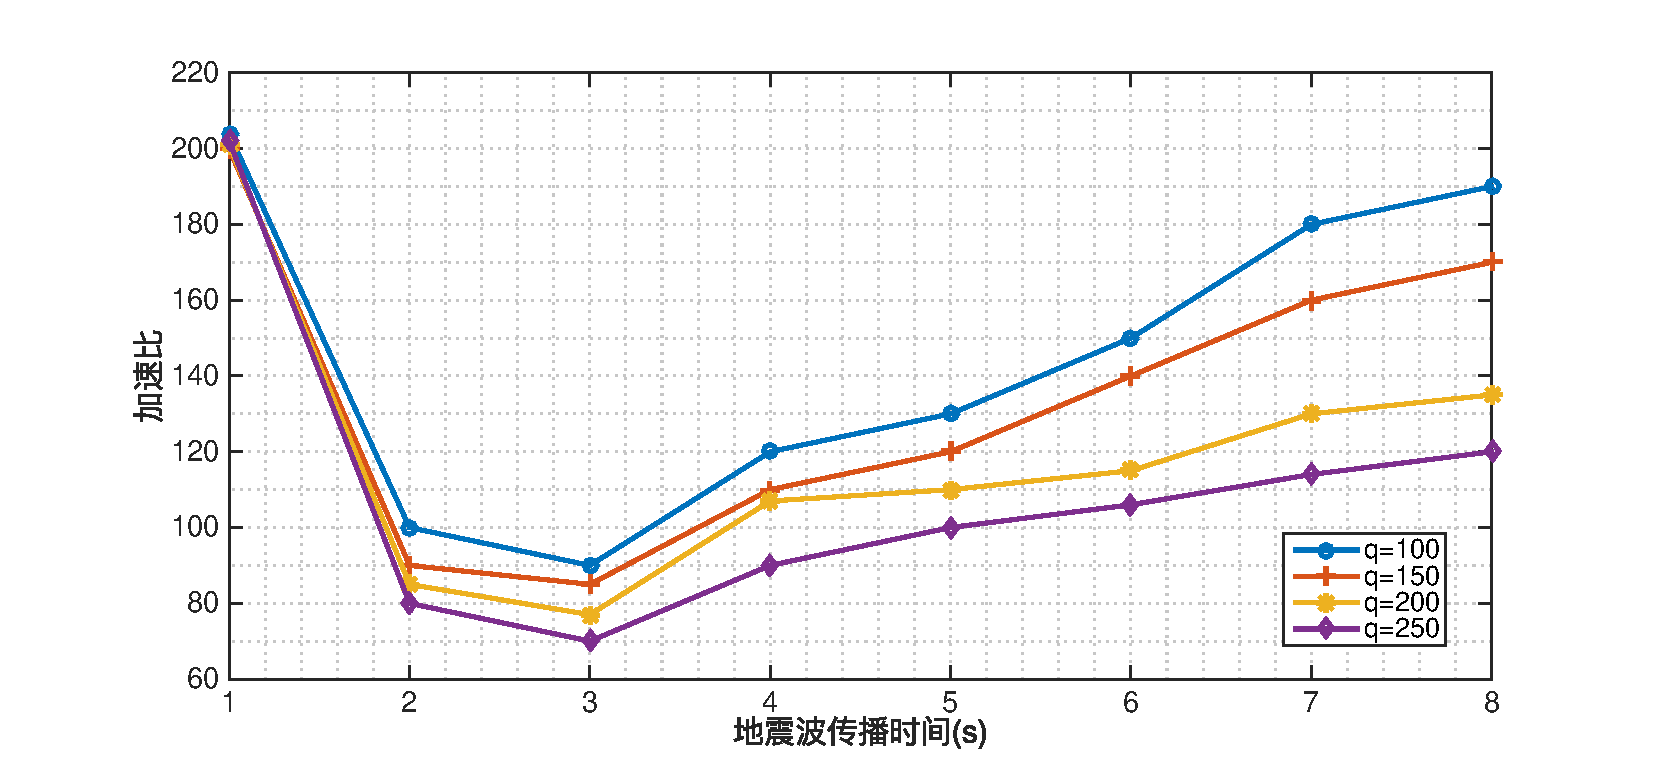
\includegraphics[width=0.9\columnwidth]{不同Q的加速比.eps}
\caption{不同Q在地震波传播不同时间点的加速比。}
\label{fig:diffqspeedup}
\end{figure}

% section 分时动态区域变分辨率正演方法 (end)

\section{集合全波形反演方法}

\subsection{设计思路}
全波形反演方法(full waveform inversion; FWI)于1984年由Tarantola提出,能准确地从人工地震记录中提取大量地下介质信息\cite{tarantola1984inversion,plessix2012full,brossier2009seismic}。该方法通过对比数值模拟合成的地震记录和实际观测的人工地震记录误差,迭代更新模型参数,从而反演地下介质模型\cite{yushu}。然而,由于该方法伴随着巨大的计算开销,直到2010年超级计算机和NVIDIA GPU,Intel MIC等加速器的兴起,为全波形反演方法提供了足够的算力,该方法才逐渐成为研究热点,并为各大石油公司采用。

尽管全波形反演方法在理论上能够很好地反演地下介质模型,但在实际生产中却面临着两大问题。一方面,全波形反演方法需要非常准确的初始速度模型作为输入,否则该算法很容易陷入局部最优\cite{virieux2009overview}。虽然地震记录中的低频信号成分能够降低对初始速度模型的要求,但是在实际生产场景中往往很难捕捉到低频信号\cite{sirgue2006importance}。另一方面全波形反演方法对地震记录数据中的噪音非常敏感,这严重影响了该算法的实际成像效果。

集合全波形反演方法(EnKF)\cite{yushu,he2015ensemble}在传统完全反演\cite{tarantola1982generalized}(total inversion)的基础上,通过使用集合卡尔曼滤波\cite{evensen2003ensemble}中的集合协方差来近似完全反演中协方差算子,这降低了在完全反演中更新协方差算子的计算开销,使之可以在一般的分布式集群中进行计算。然而,由于速度模型中需要更新的参数数量比集合样本数量大2-4个数量级,集合卡尔曼滤波的更新增量受到很大的限制。对此,集合全波形反演方法再次引入了震源编码技术\cite{krebs2009fast}。震源编码技术将所有的震源和地震记录分别进行叠加,每次叠加时不同的震源和地震记录分别使用不同的震源编码,在有利于克服局部收敛的同时\cite{castellanos2014fast},也克服了集合卡尔曼滤波低秩空间的局限性。

\subsection{算法描述}
均匀介质的声波全波形反演方法可以通过方程\ref{eq:fwi}表示:
\begin{equation}
\label{eq:fwi}
  \min_{m} \phi(m) = \sum_{i=1}^S \rho(\mbox{H}_i(m) - d_{i} ),
\end{equation}
其中$m$表示背景速度模型,$\rho(\cdot)$是一个补偿函数,$d_i=d_1, \ldots, d_S$表示观测数据(实际接收的地震记录),$\mbox{H}_i=\mbox{H}_1, \ldots, \mbox{H}_S$则表示与之相对应的第$i{th}$个正演算子,$S$表示总勘探实验次数(每发射一炮代表一次实验)。这个优化问题通常使用如方程\ref{eq:steepest}形式的迭代算法进行求解:
\begin{equation}
\label{eq:steepest}
m_{k+1} = m_{k} + \alpha_{k}s_k,
\end{equation}
其中$s_k$表示搜索方向,$\alpha_{k}$表示步长。常用的方法包括最速下降法、共轭梯度法等等。

集合全波形反演方法在在每次速度模型更新之后,使用集合卡尔曼滤波对速度模型集合进一步更新,如方程\ref{eq:enkfupdate}所示:
\begin{equation}
\label{eq:enkfupdate}
\left(\mbox{H}\Psi_k^{'}(\mbox{H}(\Psi_k^{'})^T)+D_k^{'}(D_k^{'})^T\right)^{-1}\approx\left((\mbox{H}\Psi_k^{'}+D_k^{'})(\mbox{H}\Psi_k^{'}+D_k^{'})^T\right)^{-1}.
\end{equation}
其中$k$表示第$k$个迭代步,$\Psi_k=(\psi_1^k,\psi_2^k,\ldots,\psi_N^k)$表示有$N$个速度模型样本组成的背景速度场,$D=(d_1^k,d_2^k,\ldots,d_N^k)$表示添加扰动之后的观测数据集合。通过SVD分解,我们有
\begin{equation}
\label{eq:svd}
\mbox{H}\Psi_k^{'}+D_k^{'}=USV,
\end{equation}
其中$U$和$V$是正交矩阵,$S$是对角矩阵。结合方程\ref{eq:enkfupdate}和\ref{eq:svd},我们获得集合更新方程\ref{eq:enkf2}
\begin{equation}
\label{eq:enkf2}
(\Psi_a)_k=\Psi_k+\Psi_k^{'}(\mbox{H}\Psi_k^{'})^TU(SS^T)^{-1}U^T(D_k-H\Psi_k).
\end{equation}
其中$\Psi_a$表示分析速度场。

\subsection{算法分析}
算法 \ref{alg:enfwicode} 以伪代码的形式描述了集合全波形反演算法。与传统的全波形反演不同,集合全波形反演算法首先需要初始化EnFWI分析步所需要的相关输入,如添加随机扰动后的背景速度场集合、观测数据以及EnFWI分析步所需要的参数(第\ref{ln:enfwiinit}行)。由于背景速度场集合是由同一个初始速度场添加扰动所得,剧烈的扰动会极大改变背景速度场,从而影响全波形反演的成像结果。因此,在进行正式的全波形反演迭代之前,需要执行一次EnFWI分析步计算(第\ref{ln:enfwi1enkf}行),以便为后续的迭代提供一个差异化且较为平滑的初始速度集合。

\begin{algorithm}[ht]
%\scriptsize
%\footnotesize
\small
\caption{集合全波形反演算法伪代码}\label{alg:enfwicode}
\begin{algorithmic}[1]
\State \textbf{//初始化背景速度场集合(vels)、观测数据(obsdata)、EnFWI分析步所需参数(lambdas, ratios)}
\State [vels, obsdata, lambdas, ratios] = init4enkf(); \label{ln:enfwiinit}
\State
\State \textbf{//根据初始速度场进行首次EnFWI分析步计算}
\State enkf\_analyze(vels, obsdata, lambdas, ratios); \label{ln:enfwi1enkf}
\State
\State \textbf{for} (iter = 1; iter < niter; iter++) \{ \textbf{//EnFWI收敛所需运行的总迭代次数} \label{ln:enfwiiter}
\State
\State \quad\quad \textbf{//nsamples为集合样本数目,每一个样本执行独立的震源编码FWI}
\State \quad\quad \textbf{for} (isample = 0; isample < nsamples; isamples++) \{ \label{ln:enfwisample}
\State \quad\quad\quad\quad \textbf{//生成震源编码,并对震源和观测数据进行统一编码}
\State \quad\quad\quad\quad codes = gen\_codec(nshots); \label{ln:enfwicodec}
\State \quad\quad\quad\quad [ensrc, endata, resd, prevgrad, curgrad] = init4essfwi();
\State \quad\quad\quad\quad \textbf{for} (ishot = 0; ishot < nshots; ishots++) \{
\State \quad\quad\quad\quad\quad\quad ensrc += codes[ishot] * srcs[ishot];
\State \quad\quad\quad\quad\quad\quad endata += codes[ishot] * obsdata[ishot];
\State \quad\quad\quad\quad \} \label{ln:enfwicodecend}
\State
\State \quad\quad\quad\quad \textbf{//基于震源编码的地震波正演,计算量最大的函数之一}
\State \quad\quad\quad\quad syndata = forward\_modeling(ensrc, vels[ismaple]); \label{ln:enfwiforward}
\State \quad\quad\quad\quad vsrc = endata - syndata; \label{ln:vsrc}
\State \quad\quad\quad\quad resd += cal\_residual(endata, syndata); \label{ln:resd}
\State
\State \quad\quad\quad\quad \textbf{//基于震源编码的伴随波场反传,计算量最大的函数之一}
\State \quad\quad\quad\quad [vdata, curgrad] = backward\_propagate(vsrc, vels[isamples]); \label{ln:enfwibackward}
\State \quad\quad\quad\quad updatedir = conj\_gradient(prevgrad, curgrad); \textbf{//计算更新梯度方向}
\State \quad\quad\quad\quad swap(prevgrad, curgrad);
\State
\State \quad\quad\quad\quad \textbf{//计算更新步长,计算量最大的函数之一}
\State \quad\quad\quad\quad alpha = cal\_steplen(ensrc, vels[isample], updatedir, resd);
\State \quad\quad\quad\quad update\_vel(alpha, updatedir, vels[isample]); \textbf{//根据梯度和步长更新背景速度场} \label{ln:enfwibackwardend}
\State \quad\quad \} \label{ln:enfwisampleend}
\State
\State \quad\quad \textbf{if} (iter \% enkf\_interval == 0) \{ \textbf{//每隔enkf\_interval迭代步进行EnFWI分析步计算} \label{ln:enfwienkfbegin}
\State \quad\quad\quad\quad enkf\_analyze(vels, lambdas, ratios);
\State \quad\quad \} \label{ln:enfwienkfend}
\State \} \label{ln:enfwiiterend}
\end{algorithmic}
\end{algorithm}

集合全波形反演方法与传统全波形反演的计算流程类似,都是通过迭代算法来求解(第\ref{ln:enfwiiter}到\ref{ln:enfwiiterend}行)。但由于集合全波形反演方法使用集合样本来替代传统全波形反演中的独立样本,集合全波形反演方法需要对集合中的每一个样本独立执行完成的FWI计算(第\ref{ln:enfwisample}到\ref{ln:enfwisampleend}行)。这是集合全波形反演方法引入额外计算开销的最主要原因。集合中的每一个样本都是一个独立的完整全波形反演计算,因此集合全波形反演的计算复杂度与集合的样本数量成线性相关。为了降低计算复杂度,集合全波形反演方法引入了震源编码,在每一个迭代步每一个样本中对所有震源和观测数据进行震源编码(第\ref{ln:enfwicodec}到\ref{ln:enfwicodecend}行),然后对编码后的震源进行线性叠加。未进行震源编码时,全波形反演需要遍历每一炮勘探实验,而进行震源编码之后,不再需要逐炮进行遍历,而是将不同位置的震源根据震源编码同时添加到地震波场中。震源编码技术直接将全波形反演的计算复杂度将为原来的$1/nshots$,其中$nshots$表示炮的数目。这在大规模三维石油勘探中的加速效果非常明显,因为大规模石油勘探中炮击的次数通常为成千上万甚至十万个。值得注意的是,在每个迭代步每个样本的全波形反演中,所有炮击的震源和观测数据使用相同的编码,但在不同迭代步不同样本中,却需要重新生成编码。

随后,以编码后的震源和当前样本速度场作为输入进行地震波正演(forward\_modeling),模拟地震波从震源发射,传播经过不同地下介质,最后到达地震记录接收器的整个过程(时间从$t=0$到$t=nt-1$时刻,第\ref{ln:enfwiforward}行)。由于当前速度场并不是真实的速度场,以此速度场进行正演得到的地震记录成为合成地震记录(syndata)。通过实际观测地震记录和当前合成地震记录,计算可得伴随波场震源(vsrc)和目标函数残差(resd,第\ref{ln:vsrc}行和第\ref{ln:resd}行)。全波形反演的目标则在于最小化目标函数残差,残差越小,代表当前速度模型与真实速度模型越接近。以伴随波场地震和当前速度模型作为输入进行地震波反传(时间从$t=nt-1$到$t=0$时刻),并与对应的正传波场进行相关(correlation)操作,可以求得速度场更新的梯度和步长,用以更新当前速度模型(第\ref{ln:enfwibackward}到\ref{ln:enfwibackwardend}行)。在整个基于震源编码的全波形反演中,计算量最大的三个过程分别是地震波正传、伴随波场反传和计算更新步长。每一个过程都需要对整个波场进行从$t=0:nt-1$或$t=nt-1:0$进行更新。时间步长越短、计算网格分辨率越高或者有限差分算子长度越大都会急剧增大波场更新的计算量,给现代并行计算机带来巨大的挑战。更新波场的过程将在下文详细介绍。对集合中的每一个速度场使用基于震源编码的全波形反演进行更新之后,每隔一定的迭代步,执行集合卡尔曼滤波分析以进一步更新背景速度场集合(第\ref{ln:enfwienkfbegin}到\ref{ln:enfwienkfend}行),然后进入下一个迭代步。

集合卡尔曼滤波的分析步旨在利用集合替代样本,降低初始速度模型和数据噪音对对算法收敛的影响,提高算法的收敛域。集合全波形反演的额外开销一方面来源于使用集合替代单独样本,在全波形反演中需要为集合中的每个样本单独更新背景速度场。然而,在引入了震源编码之后,震源编码对所有的炮点进行叠加,极大降低了计算复杂度,减轻甚至抵消了集合样本带来的开销。集合全波形反演另一方面的开销则是集合卡尔曼滤波分析步(简称分析步)的计算,虽然并不需要在每个迭代步中都执行分析步计算,但深入分析有利于我们更好地理解集合卡尔曼滤波分析步,并为后续的优化提供可靠的思路。

公式\ref{eq:enkf2}描述了分析速度场的更新方式。结合算法 \ref{alg:enfwicode},我们可以发现如下计算特性:
\begin{itemize}
  \item 分析速度场的更新是所有速度模拟样本的整体更新,而不是像震源编码全波形反演中的每个速度模型独立更新。这里对计算机的内存提出了重大的挑战,尤其是当集合样本数目巨大的时候。
  \item 分析速度场更新的主要计算是大型矩阵和向量代数运算,包括矩阵加法、乘法、转置、求逆等计算密集型的操作,这与太湖之光强大的计算能力十分吻合。
  \item 正演算子$\mbox{H}$,即算法 \ref{alg:enfwicode} 中的forward\_modeling函数仍旧在公式中扮演者重要的作用。通过程序用时解剖(profile)发现,正演算子$\mbox{H}$依旧是EnFWI分析步最耗时的函数,但与算法 \ref{alg:enfwicode}不同,分析步中的正演算子无需设计IO存储,因为分析步中不需要进行地震波反传操作并进行相关(correlation)操作。
\end{itemize}

\begin{table}[ht]
\centering
\caption{集合卡尔曼滤波分析步中不同计算操作耗时百分比。}
\label{tb:enkfprofile}
\begin{tabular}{ccccccc}
\hline
计算操作  & 矩阵加法  & 矩阵乘法  & 矩阵求逆   & 矩阵转置  & 正演算子   & 其他    \\\hline
所占百分比 & 3.2\% & 8.5\% & 17.0\% & 4.3\% & 58.9\% & 8.1\% \\\hline
\end{tabular}
\end{table}
表\ref{tb:enkfprofile}总结了集合卡尔曼滤波分析步中不同计算操作耗时百分比。我们可以发现,优化分析步计算的核心是优化正演算子和矩阵求逆运算。同时,需要同时考虑神威超算系统单节点较小的内存,进行适当的任务划分。



% section 实验结果与分析 (end)

\section{本章小结} % (fold)
正演的本质是仿真地震物理过程,这是地震模拟的核心,同时也是反演的基础。正演算法的性能也直接决定着反演的性能。本研究讨论基于波动方程的正演算法,从算法层面提出优化正演性能的两种方法。分时动态区域正演算法利用地震波传播初期未填充模拟区域的现象,通过分时确定最大传播范围,忽略波前未到达的区域,从而提升计算效率。分时变分辨率正演方法利用地震波能量在地球内部不断衰减的特性,结合稳定性和频散条件,分时动态改变波场时空分辨率,并从二维声波方程扩展到三维弹性波方程。随后本章将分时动态区域正演和分时变分辨率正演方法结合使用,提出分时动态变分辨率正演方法作为本研究基础正演方法。最后本章验证了分时动态变分辨率正演方法能够保证正演精度的同时获得了可观的性能提升。



% section 本章小结 (end)
% chapter 分时动态区域变分辨率正演方法 (end)
% %!TEX root = main.tex
\chapter{面向申威异构众核处理器的并行优化方法} % (fold)
\label{cha:面向申威异构众核处理器的并行优化方法}

\section{申威异构众核处理器与并行计算模型} % (fold)

\subsection{申威20610处理器概述} % (fold)
\label{sub:申威20610处理器概述}

太湖之光使用了我国自主研发的片上异构众核申威26010处理器(如图\ref{fig:sunwaycpu}所示),其中包括4个核组(Core Group,CG)\citep {fu2016sunway},每个核组包括一个主核(Management Processing Element,MPE),64个从核(Computing Processing Element,CPE)和一个内存控制器(Memory Controller, MC)。 每个申威26010处理器拥有260个计算核心,每个计算核心的主频为1.45GHz,双精度浮点运算峰值性能为3TFlops,功耗为300W。

\begin{figure}[ht]
\centering
\includegraphics[width=1\columnwidth,page=3]{SW26010架构-crop.pdf}
\caption{国产片上异构众核申威26010处理器架构。}
\label{fig:sunwaycpu}
\end{figure}

申威处26010理器的主核和从核均采用64位精简指令集。主核与Intel核心类似,可以在内核态和用户态执行,支持中断、乱序执行、内存管理等功能,适用于执行调度、管理、通信和IO等功能。从核在主核的基础上进行精简,只在用户态运行,不支持乱序执行、中断等管理功能,只支持简单的分支预测。每个核组中的64个从核组成$8\times8$从核阵列,阵列中每一行和每一列各拥有一条数据总线,总线连接的从核可通过寄存器通信方法共享数据。

\begin{figure}[ht]
\centering
\includegraphics[width=.8\columnwidth]{memory_hieararchy-crop.pdf}
\caption{CPE的内存层次结构。顶层是高效的寄存器,访问或通讯需要花费1或11个周期;中间是大小为64KB的LDM高速缓存,访问LDM需要4个周期;底层是所有从核共享的8GB主存,访问需要120+个周期,带宽为136GB/s。}
\label{fig:sunway_mem}
\end{figure}

图~\ref {fig:sunway_mem}描述了申威26010处理器的内存层次结构和访问延迟。每个申威CPU的4个核组配备32GB内存,每个核组包含一个内存控制单元(memory controller, MC),可以访问8GB内存。在目前这一代申威处理器中,每个核组连接到一个带宽为34 GB/s的DDR3接口。 虽然每个申威处理器的峰值性能可达3TFlops,但内存带宽仅为136GB/s。每个从核包含16KB的指令缓存,以及64KB的高速本地直接内存(local direct memory, LDM)。LDM高速缓存的带宽为与CPU中的L1缓存相当,但需要开发者针对不同应用进行精细的手动管理,这是应用优化的关键之一。此外,每个从核包含32个浮点寄存器与4个寄存器通信缓冲区。其中访问本地寄存器需要一个周期,通过每一行或每一列的数据总线以及寄存器通信缓冲区进行寄存器通信需要11个周期完成。良好的寄存器通信策略能有效减少全局内存访问,节约DMA数据传输带宽,提高数据复用率。

% subsection 申威20610处理器概述 (end)

\subsection{并行计算模型} % (fold)
\label{sub:并行计算模型}



神威超算支持多种并行开发模型。在不同的CPU/核组/进程间采用消息传递接口(Message Passing Interface, MPI),一个CPU的4核组也可采用线程级OpenMP模型。此外,针对神威超算异构众核结构,最适用的线程级编程模型为OpenACC和Athread。

申威处理器支持的OpenACC并行编程模型遵从OpenACC-2.0标准。OpenACC编程模型与OpenMP编程模型的设计思想类似,用户只需在核心计算循环代码块前添加OpenACC指导语句,并用自动化并行编译工具编译后可生成从核并行代码,目的是为了降低编程难度。目前除了申威处理器以外,NVIDIA公司也在大力推广OpenACC。对于NVIDIA公司而言,OpenACC的编程门槛和编程复杂度远低于CUDA,因此更易于让科学计算从业者接受。OpenACC虽然降低了编程的门槛和复杂度,但却对编译器提出了更高的要求。OpenACC的性能一方面取决了用户是否正确使用OpenACC指导语句,更重要的是取决于编译器能否将OpenACC指导语句和源代码转换为高效的并行计算代码,并充分利用硬件的各种特性提升计算性能。目前申威26010处理器的OpenACC编程模型适用于简单的循环操作,在复杂的计算中无法发挥最优性能。


Athread并行模型通过使用Athread线程库手动编写从核代码的方式细粒度地控制每一个从核。OpenACC编译器对指导语句编译的本质也是将OpenACC代码转换为Athread代码,并调用从核编译器生成从核代码。因此可以在OpenACC代码转换后的Athread代码中进行二次开发,这一定程度上能降低开发工作量。Athread线程库与Pthread线程库类似,支持对每个从核独立的计算、调度、同步等等。此外,Athread还支持申威26010处理器独有特性,如LDM高速缓存策略设计、从核间寄存器通信和向量化等等。OpenACC通常无法处理结构复杂的循环结构,Athread线程库则能达到较高的性能,但相应地提高了开发成本。

为了获得极致的计算性能,本研究使用Athread线程库进行开发,并在Athread线程库的基础上设计了一系列性能优化的方案,这将在后续的章节详细介绍。

% subsection 并行计算模型 (end)

\subsection{正演算法在申威处理器的计算挑战} % (fold)

太湖之光在2016年的首次发布\citep{fu2016sunway},标志着最领先的超级计算机的运算能力首次超过了100Pflops,运算核心首次超过1000万。而太湖之光的计算能力达到前所未有的水平,其性能相当于天河二号超级计算机的3倍,美国Titan超级计算机的5倍,然而其内存系统相对比较一般。 如图\ref{tb:supercomputer-comp}所示,太湖之光的总内存大小与其他系统相似(只比两个基于GPU的系统Piz Daint和Titan稍好),byte-to-flop的比例非常低,只有其他异构系统的五分之一,日本“京(K)"超级计算机的十分之一。 这样的一个体系成为了将科学应用扩展到下一个层次的潜在而又严峻的挑战,特别是对于需要大内存空间和高内存带宽的地震模拟问题,打破内存的局限(内存墙)成为本研究最大的挑战。

\begin{table}[ht]
\footnotesize
\caption{太湖之光超级计算机与其他领先超算系统的简要比较。$size_{MEM}$和$BW_{MEM}$分别代表内存的总量和带宽$\frac{BW_{MEM}}{PEAK}$表示计算内存带宽与系统峰值计算性能的比率。}
\label{tb:supercomputer-comp}
\center
\begin{tabular*}{0.8\columnwidth}{cccccc}
\hline\hline
   & PEAK & LINPACK & $size_{MEM}$  & $BW_{MEM}$ & $\frac{BW_{MEM}}{PEAK}$ \\
   & (Pflops) & (Pflops) & (TB) & (TB/s) & {BYTE per flop} \\
   \hline
   TaihuLight & 125 & 93 & 1,310 & 4,473 & 0.038 \\\hline
   Tianhe-2 & 54.9 & 33.9 & 1,375 & 10,312 & 0.188 \\\hline
   Piz Daint & 25.3 & 19.6 & 425.6 & 4,256 & 0.168 \\\hline
   Titan & 27.1 & 17.6 & 710 & 5,475 & 0.202 \\\hline
   Sequoia & 20.1 & 17.2 & 1,572 & 4,188 & 0.208 \\\hline
   K & 11.28 & 10.51 & 1,410 & 5,640 & 0.5 \\\hline
\hline
\end{tabular*}
\end{table}

与神威超算超大的计算规模和强大的计算能力相比,内存容量和内存带宽则是神威超算的一大不足。虽然每个节点只有32GB内存,但神威超算超过40,000个节点以及高效的网络通信,内存容量的不足可通过将应用扩展到更多的节点来弥补。神威超算每个节点的内存带宽为136GB/s,仅为Intel KNL的1/3以及NVIDIA GPU的1/5,给许多访存受限问题提出了巨大的挑战。本研究的正演算法是基于波动方程的显示时间有限差分算法,该算法的核心计算模式为$Stencil$运算,是典型的访存受限问题。在三维弹性波地震模拟涵盖了30-50个三维数组,这进一步加剧了访存的挑战。

如第\ref{sub:神威超算软硬件环境}节所述,深度的从核优化使用Athread并行模型,并合理利用LDM高速缓存。从核计算的基本流程为:(1)主存中的数据通过DMA方式传输LDM高速缓存;(2)从核访问LDM高速缓存中的数据并执行相关运算;(3)将运算结果从LDM高速缓存通过DMA方式传输到主存中。

$Stencil$计算的主要耗时在于DMA传输时间,这由两方面因素决定:DMA数据传输总量和DMA传输带宽。在神威从核运算中,每个核组有$8\times8$从核阵列,每个从核分别需要通过DMA方式将数据在主存和LDM中进行传输。与MPI通信类似,核组主存的划分方式、64个从核的处理主核数据时的逻辑排列方式,也会对DMA数据传输总量造成影响。当数组的数量增大时,影响也随之增大。


虽然神威超算每个核组的峰值内存带宽为34GB/s,然而在实际开发中,大多数应用都无法达到。DMA传输带宽与DMA传输的连续数据块大小有密切的正相关关系(如表
\ref{tb:sw-bw}所示)。由表可见,当DMA连续传输块大小不足128字节时,DMA的传输带宽不足理论带宽的一半。只有当DMA连续传输块大小超过512字节时,才可以达到较合理的内存带宽利用率。

\begin{table*}[thb]
%\renewcommand{\arraystretch}{1}
%\small
%\tiny
\caption{单核组DMA连续传输块大小对应的实测带宽(GB/s)}
\label{tb:sw-bw}
\centering
\begin{tabular}{|c|c|c||c|c|c|}
  \hline
  块大小(字节) & $Get$ & $Put$ & 块大小(字节) & $Get$ & $Put$ \\
  \hline
  32&4.31&2.56& 512&27.42&30.34\\
  \hline
  64&9.00&9.20& 576&25.96&28.91\\
  \hline
  128&17.25&18.83& 640&29.05&32.00\\
  \hline
  192&17.94&19.82& 1024&29.79&33.44\\
  \hline
  256&22.44&25.80& 2048&31.32&35.19\\
  \hline
  384&22.88&24.67& 4096&32.05&36.01\\
  \hline
\end{tabular}
\end{table*}

本研究的三维弹性波地震模拟包含30-50个数组。需要将所有的三维数组频繁读写到LDM中,读写和划分的策略影响着DMA数据传输的总量。另一方面,由于数组总量多,使得每个数组在LDM中容纳的元素很少,每次DMA操作是连续的数据块大小也很小,极大地制约了DMA传输带宽。因此,$Stencil$运算在申威处理器的性能优化主要关注于如何降低DMA数据传输总量和提升DMA传输带宽。

\section{最小DMA数据传输方案} % (fold)
\label{sec:最小DMA数据传输方案}

\subsection{单从核数据传输方案推导}

申威26010芯片高效的从核计算需要从LDM中读取数据而非从共享主存中获取,但每个从核仅有64KB高速缓存LDM,在涉及大量数组的kernel中,每个数组能够分配的LDM缓存非常有限。此外,对于stencil这类访存受限问题,从核优化的另外一个重点在于缩短数据从主存DMA传输到LDM的时间。缩短DMA传输的时间有两个方法,减少数据传输总量和提升DMA传输带宽。

在stencil的计算中,每更新一个中心点需要访问周围的其他格点。LDM空间有限,无法储存整个二维或者三维数组(波场),因此需要对波场进行划分。划分后的每个子波场包含中心波场以及边界出所需额外访问的Halo区域。不同的划分会对应不同的Halo区域,从而影响DMA数据传输总量。本小节推导出在stencil运算二维划分下最小的DMA数据传输总量。

\begin{figure}[ht]
  \centering
  \includegraphics[width=1.0\columnwidth]{单从核2D划分最小DMA传输.pdf}
  \caption{单从核2D划分最小DMA传输。}
  \label{fig:cpe-2d-derive}
\end{figure}

如图\ref{fig:cpe-2d-derive}(a)所示,设数组的大小为$NZ\times NX$,其中Z轴是数组的快轴。Halo区域的宽度为$H$,每个数组在LDM所占的空间为$S=(wx+2H)\cdot(wz+2H)$,计算所需的格点都存储在这片空间中,我们称之为LDM窗口。窗口可以沿Z轴或者X轴滑动(如图\ref{fig:cpe-2d-derive}(b)(c)所示):
\begin{itemize}
  \item 沿着X轴滑动时,原窗口最右列的Halo区域能够被新窗口完全复用,新窗口只需读取右边四列数据。
  \item 沿着Z轴滑动时,原窗口最下行的Halo区域能够被新窗口完全复用,新窗口只需读取下面四行数据。
\end{itemize}

虽然两种滑动方式的DMA传输数据量相同,但效率却有差异。但由于数组的快轴是Z轴,沿着X轴滑动时,新窗口需调用4次DMA,每次DMA的大小为5个元素;而沿着Z轴滑动时,新窗口需调用5次DMA,每次DMA的大小为4个元素。由表\ref{tb:sw-bw}可知,DMA传输的连续数据块越大能获得更大的带宽,因此窗口沿着X轴从左向右滑动更有利于提高DMA传输效率。

公式\ref{eq:单从核二维划分最小DMA传输}描述二维划分下最小的DMA数据传输总量
\begin{equation}
  \min_{wx,wz} D(wx,wz) = (wz+2H)\cdot(NX+2H)\cdot\frac{NZ}{wz},
  \label{eq:单从核二维划分最小DMA传输}
\end{equation}
其中$(wz+2H)\cdot(NX+2H)$表示每次沿着X轴滑动所需传输的数据总量,$\frac{NZ}{wz}$表示再次从左至右滑动的次数(轮数)。公式\ref{eq:单从核二维划分最小DMA传输}化简后可得公式\ref{eq:单从核二维划分最小DMA传输2}。
\begin{equation}
  \min_{wz} D_{1cpe}(wz) = (1+\frac{2H}{wz})\cdot(NX+2H)\cdot NZ,
  \label{eq:单从核二维划分最小DMA传输2}
\end{equation}

我们可以看到,$wz$与$D_{1cpe}(wz)$呈反相关,当$wz$越大时,$\frac{NZ}{wz}$越小,即再次从左至右滑动的次数越少,由于每次从左至右滑动时都需要额外读取上下边界的Halo区域,因此轮数越少,传输总量$D_{1cpe}(wz)$越小。

\subsection{64从核数据传输方案推导}
公式\ref{eq:单从核二维划分最小DMA传输2}描述的是一个从核进行DMA传输的最优情况。一个核组中有64个从核,64个从核的不同排列和划分方案也会对DMA的数据传输总量造成影响。现推导单核组64从核共同进行计算和DMA传输时,最小的传输总量。

\begin{figure}[ht]
  \centering
  \includegraphics[width=1.0\columnwidth]{多从核2D划分最小DMA传输.pdf}
  \caption{多从核2D划分最小DMA传输。}
  \label{fig:multi-cpe-2d-derive}
\end{figure}

如图\ref{fig:multi-cpe-2d-derive}所示,设每个MPI进程需要更新的网格为$NZ\times NX$,每个核组的从核按照$mz \times mx$进行划分。每个从核需要处理的网格需要进一步划分才能放进64KB的LDM中,因此对单从核内部进一步按照$pz\times px$划分,划分后的每一个小块能加载到LDM中,LDM窗口的大小为$(wz+2H)\times(wx+2H)$。我们需要推导出当$mz$和$mx$如何划分时,能够使得多从核划分下的DMA传输数据量最小。此时,每个从核LDM最小DMA数据传输的优化函数变为
\begin{equation}
  \min_{mx,mz,px,pz} D_{64cpe}(mx,mz,px,pz) = (\frac{NZ}{mz\cdot pz}+2H)\cdot(\frac{NX}{mx}+2H)\cdot pz,
  \label{eq:多从核二维划分最小DMA传输}
\end{equation}
化简可得
\begin{equation}
  \min_{mx,mz,pz} D_{64cpe}(mx,mz,pz) = (\frac{NZ}{mz}+2H\cdot pz)\cdot(\frac{NX}{mx}+2H),
  \label{eq:多从核二维划分最小DMA传2}
\end{equation}
且当64个从核都进行参与时,满足以下条件
\begin{equation*}
    \left\{\begin{matrix}
mx\times mz=64\\
1\le mz \le 64 \\
pz \ge 1 \\
1 \le \frac{NZ}{mz\cdot pz} \le Z_{max}
\end{matrix}\right.
\Leftrightarrow
  \left\{\begin{matrix}
mx\times mz=64\\
1\le mz \le 64 \\
1 \le pz \\
\frac{NZ}{mz\cdot Z_{max}} \le pz \le \frac{NZ}{mz}
\end{matrix}\right.。
\end{equation*}
其中,$Z_{max}$为每个从核LDM中最多可用来分配给Z轴的空间。将$mx=61/mz$代入到公式\ref{eq:多从核二维划分最小DMA传2}中,公式\ref{eq:多从核二维划分最小DMA传2}可得
\begin{equation}
  \min_{mz,pz} D_{64cpe}(mz,pz) = \frac{NX\cdot NZ}{64}+\frac{NZ}{mz}\cdot 2H+\frac{NX\cdot mz \cdot pz}{64} \cdot 2H + pz\cdot 4H^2,
  \label{eq:多从核二维划分最小DMA传3}
\end{equation}

(1)若$pz \ge \frac{NZ}{mz\cdot Z_{max}} \ge 1$,代入公式\ref{eq:多从核二维划分最小DMA传3}可得
\begin{equation}
  \min_{mz} D_{64cpe}(mz) \ge \frac{NX\cdot NZ}{64}+\frac{NZ}{mz}\cdot 2H+\frac{NX\cdot NZ}{64\cdot Z_{max}} \cdot 2H + \frac{NZ}{mz\cdot Z_{max}}\cdot 4H^2,
  \label{eq:多从核二维划分最小DMA传4}
\end{equation}
则$D_{64cpe}(mz) $与$mz$呈反相关,当$mz$越大,$D_{64cpe}(mz) $越小。当$mz=64, mx=1, pz = \frac{NZ}{64\cdot Z_{max}}$时,$\min_{mz} D_{64cpe}(mz=64)$最小。

(2)若$\frac{NZ}{mz\cdot Z_{max}} < 1$,则$pz\ge 1$,代入公式\ref{eq:多从核二维划分最小DMA传3}可得
\begin{equation}
\begin{aligned}
  \min_{mz,pz} D_{64cpe}(mz,pz) &\ge \frac{NX\cdot NZ}{64}+\frac{NZ}{mz}\cdot 2H+\frac{NX\cdot mz}{64} \cdot 2H + 4H^2 \\
  &\ge \frac{NX\cdot NZ}{64}+2H\cdot2\sqrt{\frac{NZ}{mz}\cdot\frac{NX\cdot mz}{64} } + 4H^2 \\
  &=\frac{NX\cdot NZ}{64}+\frac{H}{2}\sqrt{NX\cdot NZ}+ 4H^2
  ,
\end{aligned}
  \label{eq:多从核二维划分最小DMA传5}
\end{equation}
当且仅当$\frac{NZ}{mz}=\frac{NX\cdot mz}{64}$时,等号成立。此时$mz=8\sqrt{\frac{NZ}{NX}}$,$mx=8\sqrt{\frac{NX}{NZ}}$。并可推出$\frac{mx}{mz}=\frac{NX}{NZ}$。此时$pz=1$。

通过总结公式\ref{eq:多从核二维划分最小DMA传4},我们得知在充分利用所有从核进行二维划分的情况下,满足以下条件可使DMA的数据传输总量最小:
\begin{itemize}
  \item 当$pz \ge \frac{NZ}{mz\cdot Z_{max}} \ge 1$时,将64个从核按照$64\times 1$进行排布,可获得最小DMA数据传输总量;
  \item 当$\frac{NZ}{mz\cdot Z_{max}} < 1$时,从核按照$\frac{mx}{mz}=\frac{NX}{NZ},pz=1$进行排布,可获得最小DMA数据传输总量。
\end{itemize}

\subsection{基于寄存器通信的从核Halo更新}
\label{sub:寄存器通信}

最小的DMA数据传输总量的推导的前提是一个核组内的64个从核间能够进行数据交互,且交互的成本很低以至于可以忽略从核间数据交互的成本。申威26010处理器与其他主流处理器相比,最与众不同的一个功能是每个核组中的64个CPE中的寄存器通信机制。由64个CPE组成的计算核心网格中,我们有8个列通信总线和8个行通信总线,这些总线成为了CPE之间进行快速寄存器通信的通道,为不同的CPE提供了高速的数据共享能力。这为$Stencil$计算中的数据重用提供了完美的解决方案。

使用基于寄存器通信的Halo交换,在每个CG内部,CPE线程只需要加载其相应的中心计算区域,并且可以通过寄存器通信操作从相邻线程获取所需的Halo区域。但同一核组内的不同线程间的寄存器通信并不能完成所有Halo的交换,跨不同核组的边界通信仍然需要所对应的线程通过共享内存的方式从主存中通过DMA方式进行加载。

寄存器级通信是通过\emph{行、列通信总线}的一对\emph{Put}和\emph{Get}API接口来实现的。发送方CPE使用\emph {Put}操作将256位寄存器数据发送到接收方CPE的\emph{传输缓冲区},而接收方CPE使用\emph{Get}操作将256位数据从\emph{传输缓冲区}传输到本地通用寄存器中。

寄存器是从核中非常稀有且宝贵的资源。每个从核只有8个256位的寄存器可用于通信。寄存器的“发送”和“接受”是同步操作,批量发送将导致接收方缓冲区饱满,从核阻塞发送方线程的正常执行。不当的寄存器通信操作反而会降低计算性能,甚至会导致不同从核线程死锁。本研究设计了间隔收发同步通信策略实现寄存器高效通信,通信的步骤如下:
\begin{itemize}
  \item 编号为奇数的从核统一执行寄存器发送操作,将1个256位的向量发送给编号为偶数的从核寄存器缓冲区;
  \item 同时,编号为偶数的从核执行寄存器接收操作,等待其他寄存器向其发送数据;
  \item 奇数寄存器发送、偶数寄存器接收完毕之后,以同样的策略执行偶数寄存器发送、奇数寄存器接收操作;
  \item 以同样的方式通信下一个256位向量。
\end{itemize}

\begin{figure}[ht]
\centering
\includegraphics[width=0.7\columnwidth]{寄存器通信-crop.pdf}
\caption{同一核组内的64个CPE使用寄存器通信。}
\label{fig:64by1-reg}
\end{figure}

由于用于通信的总线只能连接同一行或者同一列的从核,只有在同一行或者同一列的CPE才能够进行寄存器通信。如果两个CPE分布在不同的行和不同的列中,则需要多个寄存器通信来实现数据交换。

正如在第\ref{sec:最小DMA数据传输方案}节中的推导,在大多数情况下我们采用$ 64 \times1 $的CPE线程配置。在这样的配置中,需要交换数据的多数的CPE线程将不在同一行或列中。为了解决这个问题,并尽可能减少所需的寄存器通信操作次数,我们设计了一个特定的CPE ID重新映射方案。

如图~\ref{fig:id-remapping}所示,对于奇数行,我们保持重映射的逻辑 CPE ID(括号内的ID)与原始硬件CPE ID相同(ID外部的ID括号);对于偶数行,我们则保持重新映射的逻辑CPE ID与原始硬件CPE ID相反。从核ID重新映射之后,可以快速索引到正确的目标通信从核线程号。

\begin{figure}[ht]
\centering
\includegraphics[width=0.5\columnwidth]{从核ID重映射-crop.pdf}
\caption{
从核ID重新映射方案。它确保所有相邻CPE线程间的数据交换操作。 括号外的ID是原始硬件从核ID,而括号内的ID是重新映射的逻辑从核ID。}
\label{fig:id-remapping}
\end{figure}

\section{增大DMA数据传输带宽方案} % (fold)

最小DMA数据传输方法侧重降低DMA数据传输总量,本节提出增大DMA数据传输带宽的两种方案——共位数组融合和数据布局转换,旨在缩短DMA数据传输时间。

\subsection{共位数组融合}
\subsubsection{朴素共位数组融合}

第\ref{sec:最小DMA数据传输方案}节推导出了最小DMA数据传输方案。然而,即便采用上述的最佳并行方案,由于三维弹性波介质中的地震波正演需要访问大量的数组,在只有64KB的LDM中,能够分配给每个数组的缓存空间也非常有限的。三维$Stencil$运算操作需要当前格点上下左右前后六个面相近的格点,因此载入LDM的是划分后的三维数据,这在内存中只有一个维度是连续。DMA数据传输只能沿着快轴进行多次DMA传输。在申威26010处理器中,DMA传输启动开销虽然不大,但DMA传输的效率受到DMA连续传输数据块大小的严重影响。

例如,地震波正演的速度更新内核需要读取10个不同的三维数组:$ u $,$ v $,$ w $,$ xx $,$ yy $,$ zz $,$ xy $,$ xz $,$ yz $,$ d $,分别是速度的三个分量、应力的六个分量以及密度。根据第\ref{sec:最小DMA数据传输方案}节的推导可得
\begin{equation}
\begin{aligned}
C_z &\cdot C_y = 64  \\
W_z \cdot W_y \cdot W_x \cdot N_{array} &\cdot N_{bytes\_per\_variable} < 64 \times 1024
\end{aligned}
\label{eq:wzy}
\end{equation}
其中$ N_{array} $表示当前计算函数所需的3D数组的数量,$N_{bytes\_per\_variable}$表示每个变量的字节数。为了完成空间四阶的中心差分运算,LDM缓存中至少需要沿着$x$方向加载五个平面(以第三个平面为中心,前后两个面各为差分长度)。因此$ W_x $的最小值为5。对于参数$ W_y $,因为$(W_y-2H)$是加载到LDM中的有效区域,需要将$ W_y $设置为至少9(对于$ H = 2 $)以保持Halo成本处于合理的水平。因此,在10个输入数组的情况下可以从公式\ref{eq:wzy}推导出:
\begin{equation}
W_z \cdot 9 \cdot 5 \cdot 10 \cdot 4 < 64 \times 1024\\
\label{eq:wzy1}
\end{equation}
可得$ W_z $的最大值为32。在这种情况下DMA传输的连续块的大小为128字节。由表\ref{tb:sw-bw}可知对应的带宽约为17GB/s,仅为内存峰值带宽的50\%,利用率较低。

三维弹性波正演中DMA批量传输块小的现象在二维或声波方程中并不明显。在二维声波方程中不需要考虑应力和空间分量,程序中数组的总量约为三维弹性波情景中的20\%甚至更低,这使得二维声波方程中每个数组可利用的LDM容量是三维弹性波中的5倍,DMA批量传输数据块也随着增大。不过二维声波方程扩展到三维弹性波方程虽然增大了数组的总量,但物理变量却变动较小,包含应力的增加以及速度由原来的二维扩展到三维。这启发了共位数组融合思想的提出。

仍旧以速度更新函数为例,虽然该函数涉及到10个三维数组,但这10个数组可分成3组,分别代表速度(3个分量)、应力(6个分量)和密度。三个速度分量是彼此对称的,所执行的计算操作类似。六个应力分量也是如此。本研究称这三个速度分量($ u $,$ v $,$ w $)或这六个应力分量($ xx $,$ yy $,$ zz $,$ xy $,$ xz $和 $ yz $)为共位数组(co-located array),共位数组融合则分别将三个速度分量或六个应力分量融合成一个大数组。共位数组融合的过程如图\ref{fig:naive-fusion}所示。

\begin{figure}[ht]
\centering
\includegraphics[width=0.9\columnwidth,page=1]{分块共位数组融合-crop.pdf}
\caption{朴素共位数组融合示例。}
\label{fig:naive-fusion}
\end{figure}

共位数组融合之后,从等式\ref{eq:wzy}中可以看到,只有三个单独的数组可以读取,则有
\begin{equation}
W_z \cdot 9 \cdot 5 \cdot 3 \cdot 4 < 64 \times 1024\\
\label{eq:wzy2}
\end{equation}
可得$ W_z $的最大值约为108。此时,DMA传输连续数据块大小为432字节,内存带宽利用率可提高到80%左右。 

在地震波正演的极端情况下(应力更新函数),共位数组融合技术可以将DMA传输连续快大小从84字节增加到512字节,从而将有效内存带宽从50.47 GB/s提高到104.82 GB/s,极大的提升了内存带宽。

共位数组融合方法显著地提升了DMA传输的带宽,但这种数组融合方法还面临着一个问题:无法向量化。本研究称之为朴素共位数组融合方法。朴素共位数组融合方法可以将任意数量的数组进行融合,由于不同数组的元素相互交错排列而无法实现向量化。虽然向量化对$Stencil$等内存受限运算无显著的性能提升,但能显著提升计算受限的问题(如矩阵运算、卷积运算)的计算效率。本研究在朴素共位数组融合的基础上提出分块共位数组融合,使之支持向量化。

\subsubsection{分块共位数组融合}

申威26010处理器支持位宽为256比特的向量化操作,等价于支持4个连续double类型元素的算术运算。申威处理器建造之初为了更好的支持双精度浮点数的科学运算,向量化操作并不区分双精度和单精度,因此尽管单精度浮点数的位宽只有双精度浮点数的一半,申威处理器也支持4个连续float类型元素的向量化运算。分块共位数组融合策略以4个连续的元素为一个单元块,然后使用朴素共位数组融合,融合过程如图\ref{fig:block-fusion}所示。


\begin{figure}[ht]
\centering
\includegraphics[width=0.9\columnwidth,page=2]{分块共位数组融合-crop.pdf}
\caption{分块共位数组融合示例。}
\label{fig:block-fusion}
\end{figure}

不管需要融合的数组数量为多少,始终以同一个数组的4个元素为一块,保证向量化的正常运算。

\subsection{数据布局转换} % (fold)
\label{sub:数据布局转换}

共位数组融合方案能有效增大DMA数据传输块大小,但只适用于能够融合的数组,如速度的三个分量、应力的六个分量以及其他具有相同读写模式的变量。然而在完整的大地震模拟程序中,并非所有变量都能参与融合。对于不能进行数组融合的变量,DMA数据传输仍旧面临着传输数据块小的困境。本小节针对个别无法参与共位数组融合的变量提出另外一种增大DMA数据传输块大小的方法——数据布局转换。

数据布局转换方法根据特定的从核划分方案对数组进行预处理,重排数组中的元素,使之在从核读写时能够增大DMA数据传输块大小。数据布局转换的基本思想如图\ref{fig:layout-trans}所示。在原始的并行策略中,每个从核需要读写对应的分块(如图\ref{fig:layout-trans}(b))所示,由于原始数据在内存中的排列仅沿着一个维度连续,每个从核仅能通过多次读取小块来加载从核所需的2D平面。每次DMA传输的连续数据块小,DMA性能低下。

为了保证每个从核所需的2D平面数据在内存中是连续的,在初始化阶段每个从核首先对自己需要处理的2D平面数据进行数据布局转换,转换后的结果如图\ref{fig:layout-trans}(b)所示,转换过程如下:

\begin{itemize}
  \item 主核为需要执行数据布局转换的数组新开辟空间。由于每个从核需要执行$Stencil$运算,新开辟的空间能够容纳$Stencil$运算中的Halo部分。
  \item 需要处理完整数据边界的从核从主存中读取边界,处理中心区域的从核的Halo区域通过寄存器通信方式从邻居从核获得。
  \item 从核处理的中心区域部分则按照图\ref{fig:layout-trans}(c)所示的地址变换算法计算新的地址。
\end{itemize}   

数据布局转换后,从核DMA数据传输块的大小从原来的$wz$变为$wz\times wy$,通常情况能够获得很好的DMA带宽。

\begin{figure}[ht]
\centering
\includegraphics[width=1\columnwidth,page=1]{datalayouttransform-crop.pdf}
\caption{数据布局转换示例。}
\label{fig:layout-trans}
\end{figure}

数据布局转换方法也有局限性,它能有效提升无法参与共位数组融合的变量。然而如果该数组在每次计算更新后需要与邻近进程通信交换边界,数据布局转换则会打破需要进行通信的元素位置。原来位于边界的元素执行地址转换之后可能位于三维数组的其他位置,边界通信时无法按照连续的内存地址索引这些元素,只能通过地址逆转换还原数据,而这将进入额外的计算和访存开销。因此本研究并不建议需要与邻居进程通信的变量使用数据布局转换策略。在真实的地震模拟中,需要执行MPI通信的物理量为速度和应力,他们可以使用共位数组融合。无法使用共位数组融合的物理量通常为介质参数如密度($\rho$),它们在整个程序中始终为常量,数据布局转换策略正好为这些数据提供了很好的增大DMA数据传输带宽的解决方案。

\subsection{内存对齐}

内存对齐是另外一种减小DMA数据传输总量的方式。而在DMA数据传输中,每次的DMA传输都按128字节对齐。未按照128字节对齐分配的数组在DMA数据传输时会降低DMA传输效率。例如,若DMA连续数据传输的大小为256字节,若主存中的数据未按照128字节对齐,则需要发起3次DMA传输,共传输384字节,有效数据为256字节。若主存中数据按照128字节对齐,则只需要发起2次DMA传输,效率为前者的1.5倍。

上文介绍的共位数组融合和数据布局转换方法并未考虑内存对齐,本小节讨论每一种方法如何内存对齐的情况。对于$Stencil$运算,从核的DMA数据传输可分为两部分,Halo区域和中心区域传输。

朴素共位数组融合的数组数量不确定,因此只能在数组起始地址按128字节对齐,每个从核的计算起始地址和边界从核的Halo起始地址无法保证按128字节对齐。只有一个从核能获得字节对齐带来的带宽收益。

分块数组融合按照向量化的要求保证每个数组有4个元素连续排列。地震模拟应用中数据类型通常使用单精度浮点数($float$),每个数组连续的字节数为16。如果正好有8个数组需要融合,则正好可实现128字节的内存对齐,然而实际情况并无法保证每次分块数组融合正好是8个数组(此处假设为7个)。对于此类情况有两种对齐方式:Halo起始地址对齐和计算中心起始地址对齐,任意一种方式都容易实现,但只能获得其中一项带宽收益。本研究提出Halo地址地址和中心计算起始地址同时对齐的方法:
\begin{itemize}
  \item Halo区域的起始地址对齐要求可以通过分配内存时按128字节对齐分配内存。
  \item 计算中心区域起始位置取决于Halo区域的长度,Halo区域的长度取决了差分算子长度和融合的数组数量。如果Halo区域的字节长度不能整除128,则计算中心区域的起始地址无法按照128字节对齐。这种情况下本研究通过扩展Halo区域长度,使之能被128整除。
  \item 尾部区域也采用同样的方式进行区域扩展,保证所有从核读取的Halo区域和计算中心区域也按照128字节内存对齐。
\end{itemize}

数据布局转换不涉及多个数组合并,因此内存对齐较为简单。首先在内存分配时保证按128字节对齐,然后调整每个从核的划分,是的每个从核读取的起始地址也按128字节对齐。

%数据布局转换的过程如图1所示,首先MPE开一个空间,之后CPE先进行中间区域的地址转换,之后判断是否为某一个边界,如果为边界则需要单独读取边界,如果不是边界则需要和邻居CPE交换边界来完成转换。而地址转换的地址转换为:首先,将整个z轴在原数组按照z4进行分层,而新数组则以z4+2H分层,但层数保持不变,旧的数组z轴长度为p_{z2}p_{z3}z_4也,即z_2,而新的数组z轴长度为p_{z2}p_{z3}(z4+2H),而y轴长度保持不变。因为我们是按照一个平面一个平面地转换,因此先计算x方向的偏移量,新数组为i_{x}p_{z2}p_{z3}(y_2+2H)(z_4+2H)。在新的数组中,数据在一个层中排列完之后再排列下一层,层的序号为(i_z p_{z3} + z_{id}),再乘以y轴长度y2+2H则为该层之前的偏移。之后在该层内部先计算y轴偏移(i_y p_{y3}+y_{id})(z_4+2H),之后再加上z轴上边界H偏移,即为该区域需要转换的首地址,而旧数组地址的计算为常规计算。之后通过拷贝操作来将旧数组拷贝到新数组。

% subsection 数据布局转换 (end)

% section 数据结构变换 (end)

\section{实时压缩/解压缩设计方案}
\label{sec:实时压缩/解压缩设计方案}
\subsection{实时压缩必要性分析与设计思路}

太湖之光超级计算机作为目前世界最快的超级计算机,系统的内存上限为1PB。有限的内存限制了神威超算能够支持数值模拟的最大问题规模和分辨率。例如,对于唐山大地震模拟,在模拟范围为$320km\times 320km \times 40km$的情况下,最高分辨率能达到$10m$。尽管这已经是同等计算区域下最高精度的模拟,但如果想支持更高分辨率的地震模拟,即便是世界最快的神威超算也无法支持。

此外,地震模拟的核心数值算法是有限差分运算,运算的效率受限于神威超算的内存带宽。内存容量和带宽并非神威超算的优势,其最大的优势是高效的浮点运算单元,但有限差分算法却无法将浮点预算单元充分利用。访存受限的数值算法和神威超算较低的byte-to-float比例形成尖锐的矛盾。

本文工作基于神威超算的特殊体系结构,提出实时压缩/解压缩设计方案,旨在解决上述挑战。压缩方案通过将程序内部变量和外部数据进行压缩,降低了神威主核内存和文件系统的容量开销,使得相同物理内存能够支持更大规模算例。另一方面,神威特殊的主从核结构、编程可控的LDM高速缓存使得压缩数据可在从核中进行解压和浮点运算。由于压缩后的数据量变小,数据通过DMA从主存传输到从核LDM的总时间也随时缩短,而压缩/解压引入的额外计算也让闲置的从核计算单元得以利用,因此较为理想地解决了第二个挑战。

图\ref{fig:compression-workflow}描述了主从核协同压缩方案计算流程。首先将外部输入数据(如震源、模型)压缩后存储在硬盘中,地震模拟程序将压缩后的数据去读到主存中,从核通过$dma\_get$等接口将数据从主存传输到从核LDM中,此时数据仍处于压缩状态;从核在LDM中对数据进行解压还原成常规的单精度浮点数,并使用浮点运算单元完成所需计算;计算完毕后再压缩结果数据,并通过$dmg\_put$等接口将结果传回主存。

\begin{figure}[ht]
\centering
\includegraphics[width=0.9\columnwidth]{主从核协同压缩方案-crop.pdf}
\caption{主从核协同压缩方案计算流程。}
\label{fig:compression-workflow}
\end{figure}

\subsection{单精度浮点数压缩算法}

压缩方案的本质是以计算时间换取内存/存储空间,势必引入额外的计算开销。大地震模拟本是计算量大、耗时长的科学应用,如果压缩方案引入的额外计算开销太高,即便能够模拟更大规模的地震算例,也不具备现实意义。因此,高效的压缩算法是也压缩方案设计中一大重要环节。

传统的压缩算法如行程长度压缩算法(Run Length Encoding, RLE)、哈夫曼编码、Lempel-Ziv等对字节流进行压缩。这并不适合有限差分运算模式。例如四阶中心差分运算需要获取中心格点以及周围的各两个格点,这在内存中是不连续的,几乎无法从压缩后的数据中索引差分计算所需的格点。因此,本文工作根据有限差分运算特殊的计算模式定制了压缩算法。

设计压缩方案的另外一个考量是选择无损压缩或是有损压缩。无损压缩能够保持计算精度但需要较大的计算量且压缩率较低,而无损压缩在牺牲适量精度的情况下获得了较低的计算开销和较高的压缩率。地震模拟的数据通常用32位单精度浮点数表示,结果以地震波快照的形式呈现,因此对数据的精度有较高的容忍度。为了提高计算效率,本文提出并采用三种有损压缩算法,在可接受精度的前提下,将32位浮点数压缩成16位浮点数。

\subsubsection{IEEE 754标准半精度浮点数压缩方法}
第一种压缩方法将IEEE 754单精度浮点数压缩成IEEE标准半精度浮点数。单精度浮点数的符号位、指数位和尾数位分别有1、8、23位,半精度浮点数的符号位、指数位和尾数位分别为1、5、10位(如图\ref{fig:ieeefloathalf}所示)。IEEE标准单精度浮点数与半精度浮点数之间的转换已有大量成熟工作\cite{van2008fast},本文工作将Scipy\cite{jones2014scipy}中的单精度-半精度浮点数转换开源代码移植到神威从核。

\begin{figure}[ht]
\centering
\includegraphics[width=0.8\columnwidth,page=1]{压缩浮点数表示形式-crop.pdf}
\caption{IEEE标准单精度-半精度浮点数表示方式。}
\label{fig:ieeefloathalf}
\end{figure}

在不考虑上溢(overflow)、下溢(underflow)、非规范化(denormalized)数的情况下,标准单精度-半精度浮点数转换核心算法如算法\ref{alg:ieeefloat}所示。
\begin{algorithm}[ht]
%\scriptsize
%\footnotesize
\small
\caption{IEEE标准单精度-半精度浮点数转换核心}\label{alg:ieeefloat}
\begin{algorithmic}[1]
\State \textbf{// 16位半精度转32位单精度}
\State uint32\_t \textbf{float16\_to\_float32}(uint16\_t h) \{
\State \quad\quad return ((h\&0x8000)<<16) | (((h\&0x7c00)+0x1C000)<<13) | ((h\&0x03FF)<<13);
\State \}
\State
\State \textbf{// 32位单精度转16位半精度}
\State uint16\_t \textbf{float32\_to\_float16}(uint32\_t f) \{
\State \quad\quad uint32\_t x = *((uint32\_t*)\&f);
\State \quad\quad return ((x>>16)\&0x8000)|((((x\&0x7f800000)-0x38000000)>>13)\&0x7c00)|((x>>13)\&0x03ff);
\State \}
\end{algorithmic}
\end{algorithm}

\subsubsection{动态指数位压缩方法}
IEEE单精度-半精度的转换算法简明高效,但由于半精度浮点数使用固定的指数位和尾数位,对于指数范围大于五位的浮点数,压缩方案会产生数值问题。另一方面,对于指数范围较小的变量,固定的五位指数位则变成了浪费。

\begin{figure}[ht]
\centering
\includegraphics[width=0.8\columnwidth,page=2]{压缩浮点数表示形式-crop.pdf}
\caption{动态指数位浮点数表示形式。}
\label{fig:ieeefloatdynamic}
\end{figure}

为了解决上述问题,本人工作提出了动态指数位压缩方法(如图\ref{fig:ieeefloatdynamic}所示)。这个压缩方法中的指数位和尾数位是动态确定的,不同的数组会得到不同的结果。指数位和尾数位的计算方法如公式\ref{eq:floatdynamic}所示:
\begin{equation}
  \begin{aligned}
    N_e &= \log(E_{max} - E_{min}) \\
    N_f &= 15 - N_e
  \end{aligned}
  \label{eq:floatdynamic}
\end{equation}
其中$N_e$表示指数位,$N_f$表示尾数位,$E_{max}$和$E_{min}$分别表示被压缩数组中元素最大可能指数位数和尾数尾数。

本方法最多可用15位表示指数(实际情况不会出现15位指数),远大于标准单精度浮点数的8位,足以保证全动态范围覆盖。对于指数范围较小数据,本方法则可为尾数部分保留更多表示位数,提高压缩后数据的精度。但是,由于涉及对数或除法运算,本方法唯一的缺点是计算成本相对较高。

\subsubsection{浮点数归一化压缩方法}
在IEEE标准的单精度浮点数表示中,大部分为归一化数(normalized value)。令符号位、指数位、尾数位分别为$S$、$E$和$F$,则归一化浮点数的数值为
\begin{equation}
  f(S,F,E) = (-1)^S \cdot 1.F^{E-127}
\label{eq:floatrepresent}
\end{equation}

浮点数归一化压缩方法对浮点数进行归一化,将同一数组的所有值归一化到1到2之间的范围(如公式\ref{eq:floatnormalized}所示),根据则归一化浮点数的表示方法(公式\ref{eq:floatrepresent})可知,该浮点数的指数位$E$恒等于127。
\begin{equation}
\begin{aligned}
  v_{normalized} &= \frac{v - v_{min}}{v_{max} - v_{min}} \\
  v_{compressed} &= (v_{normalized} << 9) >> 7
\end{aligned}
\label{eq:floatnormalized}
\end{equation}

对范围为(1,2)的浮点数进行压缩,由于指数位恒等于127,压缩时无需对指数位进行存储,只需保留符号位和尾数位即可。公式\ref{eq:floatnormalized}中将归一化后的浮点数左移9位,然后右移7位得到16位数,即为压缩后的结果(如图所示\ref{fig:ieeefloatnormalized})。值得注意的是,在左移的过程中,符号位消失,因此需要在左移之前将符号位保存在第16位尾数中。

\begin{figure}[ht]
\centering
\includegraphics[width=0.8\columnwidth,page=3]{压缩浮点数表示形式-crop.pdf}
\caption{指数位归一化浮点数表示形式。}
\label{fig:ieeefloatnormalized}
\end{figure}

上述展示的三种压缩方法仅针对地震模拟应用处理了大部分常规浮点数,并未覆盖浮点数全部范围,如$NaN$,$INF$等等,这些数值并未在地震模拟应用中出现。

\subsection{压缩算法性能与精度分析}

压缩方案本身会引入额外的计算(主要是整数运算)以及密集的内存和高速缓存访问。即使所有的压缩/解压缩操作都发生在LDM中,频繁的LDM读写也会严重降低CPE的计算效率。因此,本文工作的第一个压缩版本只能达到不压缩的1/3性能。为了降低压缩方案的性能损失,我们进行了一系列优化:

\begin{itemize}
  \item 根据不同的物理量对精度敏感度不同,在满足精度要求的情况下,选择计算复杂度较低的算法;
  \item 在从核LDM中对压缩数据执行分块解压缩,以降低减少重复解压次数和LDM读写次数。
  \item 将解压缩和计算代码紧密地(在汇编代码级别)耦合以最大化寄存器中的变量的寿命,减少对LDM的加载和存储次数;
\end{itemize}

将压缩方案与地震波传播内核相结合并经过深度优化后可获得24\%的计算性能提升。这是因为压缩方案可以使得在相同的物理带宽情况下处理更多的数据。换而言之,对于地震波传播这类访存受限问题,压缩方案使得需要处理的数据总量降为原来的一半,极大地缩短了DMA数据传输时间。另一方面,在压缩率为50\%(32位浮点数压缩为16位数)的情况下,神威超算上可解决的最大问题规模扩大了一倍。这是一种通过软件形式突破硬件内存限制的方法。

实时压缩算法的精度对地震模拟有至关重要的影响,本研究通过理论和实践分析每个变量的精度敏感性,为其定制合适的压缩算法。经过精细的调优操作为不同变量选取了可接受精度范围内最大化性能的压缩算法。压缩算法的精度算例分析将在唐山大地震算例中详细描述。

% 流水线指令重排优化

% chapter 面向申威26010异构众核架构的并行优化方法 (end)
% %!TEX root = main.tex
\chapter{面向神威超算系统的大规模并行优化方法} % (fold)
\label{cha:面向神威超算系统的大规模并行优化方法}

\section{神威超算系统概述} % (fold)
\label{sec:神威超算系统概述}

\subsection{神威超算软硬件环境}
\label{sub:神威超算软硬件环境}
神威·太湖之光超级计算机系统是“国家863”重大科研专项的研究成果,是第一台全部采用国产处理器,也是世界上首台峰值性能超过100 Pflops的超级计算机。神威·太湖之光自2016年6月起已经连续4次获得Top500排名冠军。表\ref{tb:sunwaystat}描述了神威·太湖之光超级计算机系统参数:全机峰值性能为125 Pflops,内存总容量为1.31 PB,缓存总带宽为5,591 TB/s,网络链路传输带宽为14 GB/s,磁盘容量为20 PB,IO聚合带宽为341 GB/s,性能功耗比为6.05 Gflops/W。

% Please add the following required packages to your document preamble:
% \usepackage{graphicx}
\begin{table}[ht]
\centering
\caption{神威·太湖之光超级计算机系统基础参数}
\label{tb:sunwaystat}
\resizebox{\textwidth}{!}{%
\begin{tabular}{ccccccc}
\hline
峰值性能      & 内存总容量  & 缓存总带宽    & 网络带宽   & 磁盘容量 & IO聚合带宽  & 性能功耗比        \\ \hline
125Pflops & 1.31PB & 5,591TB/s & 14GB/s & 20PB & 341GB/s & 6.05Gflops/W \\ \hline
\end{tabular}%
}
\end{table}

神威·太湖之光由高速运算系统、高速互联网络和网络存储系统组成(如图\ref{fig:sunwayarch}所示)。高速运算系统由40,960个节点组成,其中每8个节点组成一个计算板,32个计算板以全连接的方式组成一个超节点,4个超节点构成一个机柜,40个机柜通过高速互联组成了峰值性能超过125 Pflops的神威超算。神威超算采用Lustre并行文件系统,通过高速互联网络与运算系统连接。神威超算的计算节点通过InfiniBand网络相连,节点间双向传输带宽为14 GB/s,全网双向带宽为56 GB/s。超节点内使用全连接网络,超节点间则使用两层胖树结构网络相连。

\begin{figure}[ht]
\centering
\includegraphics[width=.9\columnwidth]{太湖之光系统架构图-crop.pdf}
\caption{神威·太湖之光超算系统架构图。}
\label{fig:sunwayarch}
\end{figure}

神威·太湖之光的软件系统架构如图\ref{fig:sunwaysofts}所示,包含了底层的并行操作系统环境与高性能存储管理系统、国产众核CPU基础软件、并行语言及编译环境、并行开发环境与并行应用。作为主要支持大型科学计算的超级计算机,神威·太湖之光支持C/C++和Fortran等常用编程语言,并提供了完备的基础函数库(如C标准库、加速线程库、数学库等),且支持了循环级向量化。

\begin{figure}[ht]
\centering
\includegraphics[width=.8\columnwidth]{太湖之光软件系统-crop.pdf}
\caption{神威·太湖之光软件系统架构图。}
\label{fig:sunwaysofts}
\end{figure}

\subsection{神威超算与其他领先超算的比较}

神威·太湖之光超级计算机采用了与传统超算(纯CPU、CPU+GPU、CPU+MIC等)完全迥异的架构——申威26010架构,每个节点包含4个主核和256个从核。神威超算的峰值计算性能、持续计算性能、节点数和计算核心数都大幅领先其他超算系统,,分别是排名第二的天河二号的2.3、2.7、2.56、3.4倍(如表\ref{tb:system-comp}所示)。然而与计算能力相比,神威超算在内存方面在并没有太大的优势,其总内存容量为1,310 TB,略低于天河二号的1,375 TB。由于神威超算节点数目众多,因此每个节点可用内存也低于其他超算。此外,神威超算单节点的内存带宽仅为136 GB/s,而领先的Intel KNL 7250芯片的内存带宽为562GB/s,NVIDIA P100 GPU的内存带宽为732GB/s,因此神威超算的优势在于强大的单节点运算能力和众多的节点数目。对于访存受限的应用,由于神威超算的内存带宽较低,其优化面临着更严峻的挑战。

\begin{table}[ht]
\centering
\caption{神威·太湖之光超算系统与其他超算系统比较}
\label{tb:system-comp}
\resizebox{\textwidth}{!}{%
\begin{tabular}{cccccccc}
\hline
超算系统    & 峰值性能     & 持续性能     & 节点数  & 核心数      & 处理器架构     & 内存容量        & 能耗     \\
        & (Pflops) & (Pflops) &        &            &           & (TB) & (kW)   \\ \hline
神威·太湖之光    & 125      & 93       & 40,960 & 10,649,600 & MPE + CPE & 1,310     & 15,371 \\
天河二号    & 55       & 34       & 16,000 & 3,120,000  & CPU + MIC & 1,375     & 17,808 \\
Titan   & 27       & 18       & 18,688 & 560,640    & CPU + GPU & 710       & 8,209  \\
Sequoia & 20       & 17       & 98,304 & 1,572,864  & CPU       & 1,572     & 7,890  \\
Cori    & 28       & 14       & 9,152  & 622,336    & CPU       & 878       & 3,939  \\
\hline
\end{tabular}
}
\end{table}

综上所述,神威超算独特的片上异构众核架构、强大的计算能力和众多的节点数目在扩展性、访存效率等角度为应用提供了巨大优化空间。因此,本文工作将其作为主要研究平台,从应用算法、内存带宽、从核优化、扩展性、通信和IO优化多方面出发,为地震模拟研究提供高性能计算支持。第\ref{cha:面向申威异构众核处理器的并行优化方法}章介绍了面向申威处理器的应用算法、内存带宽和从核优化,本章研究面向神威超算的大规模并行优化,分别从扩展性、通信和IO等角度进行介绍。

\section{多层级并行设计方案}
\label{sec:多层级并行设计方案}

\subsection{并行任务划分基本原则}

当地球物理勘探应用需要处理较大区域的地震资料时,单节点计算机无法满足应用软件所需的计算和内存需求,并行计算机系统应运而生。例如,在一次典型的石油勘探中,勘探区域大小通常为100km $\times$ 100km $\times$ 60km,空间分辨率为20m,在不考虑边界的情况下,计算网格的格点数为$7.5\times10^9$。石油物探应用通常使用单精度浮点数表示每个格点的数值,因此完整的勘探区域的数组大小约为$3\times10^{10}$字节,即30TB,远远超出了单节点内存上限。因此只有通过对勘探区域进一步分解,使用并行计算系统才能完成所有运算。

传统并行计算通常采用单指令多数据(SIMD)并行模式将完整的大规模数据分解成若干小数据,并将其分配到不同的节点进行计算。在同构集群中,常用的并行策略包括纯MPI并行和MPI-OpenMP混合并行;在异构的GPU集群中,通常采用MPI-GPU并行方式。

神威超算拥有超大规模的40,960个计算节点,计算节点间通过Infinite Band网络相连。每个节点包含4个核组,每个核组又由1个主核和64个从核组成。核组间可以通过MPI进行进程级别的通信,从核间既可以通过共享主存交换数据,还可以通过神威架构独有的寄存器通信特性进行通信。与传统异构集群相比,神威超算的不同处理单元层次更加鲜明,不同处理单元的计算和通信方式各不相同,这为如何将科学应用进行合适的任务划分以高效扩展到神威超算的所有节点提供了巨大的探索空间。

任务划分的基本思想是将完整的大计算任务分解成若干小任务并派发到不同的节点并行计算。在多节点计算时,节点间的数据交换通过网络或者存储来完成,其效率一般会低于节点内的数据交换。计算完毕后,将结果汇集到主计算节点而形成最终计算结果。并行任务划分决定着通信方式、通信量和通信粒度,因此良好的任务划分是大规模并行计算的关键。并行任务划分通常遵循以下基本原则:
\begin{itemize}
  \item 分配给每个计算节点的任务尽量均衡。一般的并行计算机系统采用相同的节点连接而成,每个节点的处理能力相当,如果出现某个节点需执行大量任务,则其他节点必然会闲置等待,造成负载不均衡,影响整体运算性能;
  \item 尽量降低节点间通信开销。将一个完整的大问题分解成若干小问题的计算过程中,经常需要引入节点间额外的数据交换开销。在小规模并行计算中,通信不会成为主要的应用的瓶颈,但是当并行规模达到成千上万甚至十万百万量级时,通信的开销将变得不可忽略。有限的通信带宽与随之而来的通信延迟将极大降低通信的效率,此时通信甚至会成为主要的瓶颈。因此,采取适当的划分方法降低节点间通信的开销能够有效缓解通信瓶颈。此外,在大规模的并行应用中,还应该尽可能避免大量集合通信。集合通信要求不同进程在程序运算时特定时间点进行同步,而不同进程几乎很难在同一时刻到达集合通信点,会出现先到达的进程等待的现象,而先到达的进程又有可能在下次集合通信点晚点到达,导致不同进程交叉等待,降低了超算不同资源的利用效率。使用异步的非集合通信能够有效地避免这个困扰。
  \item 充分利用寄存器通信。申威处理器寄存器通信特性为从核间的数据交互提供了高效的通信手段。使用寄存器通信,从核间的数据交互无需通过共享主存来完成,有利于降低DMA数据传输负担,节约DMA数据传输带宽。
\end{itemize}

在遵循上述原则的基础上,本研究结合地震模拟的真实应用场景,提出了多层级并行任务划分方案。该方案不仅适用于地震模拟应用,还适用于其他大规模规整网格的科学问题,尤其是基于$Stencil$运算的问题。

\subsection{多层级并行任务划分}

本小节首先介绍大规模$Stencil$运算的二维区域划分方法,该思想可以灵活扩展到三维$Stencil$区域划分,这将作为下文多层级并行任务划分的基础。

图\ref{fig:2ddecomposition}为二维MPI区域划分与一维从核计算划分示例。如图\ref{fig:2ddecomposition}所示,完整的地震波场可按照不同颜色划分成四块,其中白色表示边界,也可表示Halo区域。每一个子波场派发给不同的计算核组(在使用神威超算大内存的情况下,也可以使用整个CPU替代四个核组),四个核组独立更新子波场,并在需要时更新Halo区域。在单核组处理可调用64个从核加速运算。64个从核也可以按照不同的排列方式参与运算,不同的排列方式会影响数据从主存传输到从核LDM的开销以及不同从核间寄存器通信的开销。按照第\ref{sec:最小DMA数据传输方案}节的推导,此处从核使用一维排列方式。

\begin{figure}[th]
  \centering
  \includegraphics[width=1.0\columnwidth]{2ddecomposition.pdf}
  \caption{二维MPI区域划分与一维从核排列。}
  \label{fig:2ddecomposition}
\end{figure}

在三维弹性波正演过程中,更新速度和应力的核函数包括20-50个覆盖完整区域并涉及读写的变量数组。许多适用于X86平台或GPU平台的优化技术,如3.5D blocking等方案\citep {nguyen20103},都由于极高的内存容量要求而不适合申威芯片。本文通过深入剖析神威超算的架构特点,从核组间、核组内、从核间、从核内等多个维度出发,提出了多层级并行设计方案(如图~\ref{fig:dd}所示),能高效地将地震波传播模块扩展到160,000核组,取得接近线性的扩展性,同时最大限度地降低了相关内存成本。多层级并行设计方案包括以下四部分。

\begin{figure}[ht]
\centering
\includegraphics[width=0.9\columnwidth]{blocking-crop.pdf}
\caption{多层级并行设计方案:(1)MPI进程的二维分解; (2)每个核组内分解;(3)Athreads的二维分解;(4)LDM缓存方案。}
\label{fig:dd}
\end{figure}

基于核组间的二维区域分解。三维地震模拟通常将$ z $轴(垂直方向)作为最快轴,将$ y $轴作为第二快轴,并将$ x $轴作为最慢的轴。在典型的地震模拟情景中,$ x $和$ y $(一般是几百公里)的尺寸通常比$ z $(一般是几十公里)大得多。因此在第一级划分中,为了尽量减少进程之间的通信以及增大DMA传输带宽,本文工作将地震模拟区域沿$x$和$y$轴划分为$ M_x \times M_y $个不同的分区,每个分区对应特定的MPI进程并分配给独立的核组进行计算,在AWP-ODC\citep{cui2010scalable}计算与通信重叠的基础上,本文工作还包括了许多针对神威特殊架构的优化,如基于从核的内存拷贝。基于核组间二维区域分解的地震传播模块最高以97\%的效率扩展到神威超算整机,即160,000(400$\times$400)个MPI进程。

基于核组内的二维区域分解。虽然每个核组的内存为8GB,但每个从核LDM高速缓存只有64KB,无法直接把第一级划分后的区域全部加载到LDM中运算,需要经过二次划分以确立每个从核的计算区域。本文工作将核组内的数据沿着$ y-z $方向进行二维区域分解(第二级划分)。划分后的每一块的数据能够通过DMA传输到每个从核的LDM高速缓存中并参与计算。每个从核依次遍历所有分块即可完成全部计算。

基于从核间的二维数据分解。申威架构中,高效的从核计算需要依托于高效的数据访问,因此必须将计算所需的数据提前传输到每个从核64KB的LDM高速缓存中。使用从核完成有限差分运算,每个核组中64个从核不同的逻辑排列方式对应着主存中不同的数据范围以及不同的DMA数据传输总量。本文工作采用第\ref{sec:最小DMA数据传输方案}节的最小DMA传输方案对从核进行排列,每个从核使用Athread线程沿着$ x $方向迭代,以实现不同线程高效的数据访问和DMA数据传输。

基于从核内的一维数据分解。每个从核使用DMA操作将合适大小的计算区域(中心部分和Halo区域)加载到LDM中参与运算。为了提高数据复用率和DMA传输效率,DMA操作在首次加载完毕后沿着$x$轴方向移动,每次加载一个$y-z$平面。由于$x$轴是慢轴,加载$y-z$平面能最大限度的利用数据在内存中的连续性,提升DMA传输效率。此外,不同从核的DMA数据传输虽然共享内存带宽,但从核间的DMA操作与计算过程却是异步的,能实现计算通信重叠,进一步提升效率。

\section{大规模并行通信优化方案}

当并行规模扩展到上万进程或者几十万进程时,应用的通信总量、通信链、延迟也随之增大,应用的热点会逐渐从计算转移到通信,通信开销甚至会成为整体应用的主要瓶颈。大规模并行通信优化的策略与第\ref{cha:面向申威异构众核处理器的并行优化方法}章的内存性能优化策略类似,也从三方面出发:计算通信重叠、减少通信总量与增大通信带宽。

\subsection{计算和通信重叠}
\label{sub:计算和通信重叠}
计算和通信分别占用了不同的资源,两者理论上可以并行执行以缩短计算和通信的时间。在同步MPI通信模型中,当前进程需要将更新后速度子区域边界发送给邻居进程,同时也需要从邻居进程接收边界。通信完毕后才能执行应力的更新。同步的MPI通信模型在任意时刻只有计算或者通信单一资源被利用,效率不高。本研究采用异步MPI通信模型,通过添加两层虚拟网格实现计算和通信重叠。

在图\ref{fig:2ddecomposition}所示的区域划分中,每个MPI进程需要在每个迭代步结束之后统一执行Halo区域的更新,这涉及到同步的MPI操作,会导致不同的进程在不同的迭代步交叉等待。为了进一步提升整体性能,本文为每个MPI进程设计了Halo区域更新异步通信,如图\ref{fig:comp-comm-overlap}所示。

\begin{figure*}[ht]
    \centering
    \centering
    \includegraphics[width=0.6\textwidth]{comp-comm-overlap.pdf}
    \caption{在边界添加两层虚拟网格实现异步MPI通信。}
    \label{fig:comp-comm-overlap}
\end{figure*}

与图\ref{fig:2ddecomposition}相比,图\ref{fig:comp-comm-overlap}中每个核组处理的区域中包含内部主要计算部分、Halo区域和Halo交换缓冲区。按照以下步骤完成Halo区域的更新,并实现计算通信重叠:
%(如图\ref{fig:comp-comm-impl}所示)。

\begin{itemize}
  \item 每个MPI进程调用异步MPI通信接受接口($MPI\_Irecv$),接收发送给当前MPI进程的Halo数据,并将其存储在交换缓冲区中(绿色)。由于调用的是异步接口,主线程立即返回执行后续计算。
  \item 每个MPI进程首先计算子区域的Halo区域(蓝色),使用异步MPI接口($MPI\_Isend$)把Halo区域发送给当前进程邻接的四个(二维划分)或六个(三维划分)进程,待发送的Halo区域将被复制到MPI缓冲区中独立发送,此时该进程无需等待Halo区域发送完毕而继续执行后续计算。
  \item 每个MPI核组的从核对内部区域(红色)进行有限差分计算,更新波场。此时的计算上一步的MPI发送是异步并行的,实现了计算与通信重叠。
  \item 当需要更新下一个波场(别的变量)或者下一个迭代步时,调用MPI同步接口($MPI\_Waitall$),保证上述的发送和接收数据达到指定的目的地。值得注意的是,在进程发出异步发送Halo区域数据时,MPI的通信和后续的计算并行执行,因此在调用$MPI\_Waitall$接口时,Halo区域数据已部分到达或者完全到达,取决于通信和计算的开销比例。
  \item 将交换数据缓冲区中的Halo数据复制到实际Halo区域,并进入下一个迭代步。
\end{itemize}

这种区域划分和及通信方式能够获得很好的可扩展性,尤其在有限差分算子长度较短的情况下。首先,每个MPI进程分配到的区域大小是相同的,需要进行通信的Halo区域数据大小也完全相同,不会出现负载不均衡。其次,完整区域的更新由每个小区域的更新构成,无需进行全局通信操作。不管应用扩展到多大的规模,每个MPI进程只需要发送和接收与其邻接的四个或者六个进程的数据,即便出现不同进程运行速度不同,相距较远的进程由于无需数据通信不会相互等待。

\subsection{虚拟网格}

大规模正演的主要延迟来源于不同计算节点间的数据通信。在三维弹性波正演的每个迭代步中需要进行三个速度分量和六个应力分量的边界通信。根据第\ref{sec:多层级并行设计方案}节的介绍,本文工作对完整地震区域进行二维划分(x-y方向),则通信发生在(1:nx, 1:ny, 1:NZ)子区域,其中nx、ny表示每个进程内x-y方向的范围,NZ表示完整区域的深度。二维划分下每个进程(边界除外)需要与4个邻居交换9个变量的边界。对于13点的三维$Stencil$运算,计算每一个中心点需要索引该中心点的上下左右前后各2个格点,因此子区域的每个方向需要向外扩展两层虚拟网格(ghost cell)才能异步完成整个子区域的更新。这意味着更新大小为(1:nx, 1:ny, 1:NZ)的子区域需要大小为(-1:nx+2, -1:ny+2, 1:NZ)的网格输入。

更准确地说,在每个迭代步中,如果需要更新大小为(1:nx, 1:ny, 1:NZ)的速度子区域,则需要大小为(-1:nx+2, -1:ny+2, 1:NZ)的应力子区域。每个迭代步需要更新速度和应力,同理可得,更新大小为(1:nx, 1:ny, 1:NZ)的应力子区域,则需要大小为(-1:nx+2, -1:ny+2, 1:NZ)的速度子区域。

\begin{figure}[ht]
  \centering
  \includegraphics[width=0.9\textwidth]{ghost-cell-crop.pdf}
  \caption{通信缩减过程:使用额外的两层虚拟网格对速度网格进行扩展,使用(-3:nx+4, -3:ny+4, 1:NZ)的速度子区域更新应力,然后使用(-3:nx+4, -3:ny+4, 1:NZ)的应力子区域更新速度。额外扩展虚拟网格后,只需进行三个速度分量的边界通信而无需进行应力六个分量的通信,极大地降低了通信量。}
  \label{fig:ghost-cell}
\end{figure}

本文提出的通信缩减方法在已有的两层虚拟网格的基础上额外扩展两层虚拟网格,即共四层虚拟网格(如图\ref{fig:ghost-cell}所示)。以三维速度为例,此时更新区域大小为(1:nx, 1:ny, 1:NZ)的速度子区域需要使用大小为(-3:nx+4, -3:ny+4, 1:NZ)的网格作为输入。进程间需要进行通信的的区域由原来的两层网格变成四层网格。这意味着速度网格通信后有效的区域为(-3:nx+4, -3:ny+4, 1:NZ)。额外的两层边界存储着计算应力需要的内容,这使得应力子区域的更新可以从大小为(-3:nx+4, -3:ny+4, 1:NZ)的速度网格计算得到。另一方面,由于应力网格也是用相同的方法额外扩充两层边界,应力更新后,完整的应力网格可以反过来更新当前进程的速度网格,速度和应力的计算通信过程如图\ref{fig:ghost-cell}所示。可以看到,此时只需要对速度网格进行边界通信,无需对应力网格进行通信。在三维弹性波正演算法中,速度包含三个分量,而应力包含六个分量,因此通信量约减少2/3。通信的减少有助于实现第\ref{sub:计算和通信重叠}节介绍的计算通信重叠,更利于在大规模并行时保持良好的扩展性。

虚拟网格技术与计算和通信重叠技术相结合实现了大规模运行环境下的高效通信,在本研究的唐山大地震算例中取得97.9\%的弱扩展性效率。

\section{大规模并行IO优化方案}

当并行规模逐渐增大时,IO也将逐渐成为整体应用的瓶颈。大规模的地震模拟伴随着巨大的计算量,即便拥有大型超算的支持,计算时间仍然可能需要十几个小时甚至几十个小时。更多计算核心的参与也意味着发生硬件和软件错误的概率更大。重启模块的设计正是为了解决这个问题,但在设置存储断点过程中,数十万进程需要同时将进程的内部状态变量输出到网络硬盘,这在没有优化的情况下几乎是不可实现的。为了实现大规模运行下平滑的IO操作,本文提出了IO分组、平衡IO和LZ4压缩策略。

\subsection{MPI-IO与多进程串行IO}

在大规模地震模拟中,作为输入的介质模型和震源的数据也逐渐增大并达到了几十TB量级。在地震模拟初始化时,所有的进程分别从磁盘中读取介质模型和震源。此外,在地震模拟的过程中需要定期输出波场快照或者地震记录,输出文件大小也在几百GB量级,必须使用合适的并行IO来处理巨大的输入输出。大规模并行环境中通常有两种并行IO方式:MPI-IO和多进程串行IO。

MPI-IO是MPI标准扩展提供的并行IO接口,支持多个进程共同划分同一个完整的大文件。对于规整的访问模式,MPI-IO通常能够获得很好的性能。本研究的大规模地震模拟使用了规整的介质网格,每个进程读取规整网格的子区域。依赖MPI-IO高性能库,每个进程通过定义文件视图,可以方面读取该进程所需的文件内容,即使这部分内容在文件中并非连续存储。

MPI-IO接口适用于传统的Intel、IBM或Cray处理器,因为MPI-IO都在这些处理器上进行了深度的优化,然而MPI-IO并不适合神威超算。神威超算目前并未对MPI-IO进行深入优化,性能并不理想,因此本研究使用另外一种更利于神威超算的并行IO策略——多进程串行IO。

多进程串行IO的基本思想是每个进程分别调用朴素的C/C++输入输入接口(如fread, fwrite)执行IO操作。多进程共同发起的串行IO能够充分使用文件系统代理,在块大小(block size)达到256字节时能够获得很好的性能。不过为了配合多进程串行IO方案,通常需要对完整大文件进行预处理或者后处理操作。例如,在读取介质模型时,首先对介质模型进行预处理,将完整的介质模型根据当前的MPI划分分割成若干小文件,然后每个进程读取对应的小文件。

\subsection{IO分组和平衡IO}

神威超算使用Lustre分布式文件系统,每个节点无本地磁盘。当多进程发起IO请求时,文件系统代理负责处理请求,并将IO数据写入到不同的磁盘。当进程数量达到上万甚至十万量级时,文件系统代理并发处理大量IO请求的效率较低。此外,神威超算文件系统的每个目录文件数量超过10,000时也将影响IO效率。本文提出IO分组策略,当160,000进程同时发起IO请求时,将进程分成若干组,每组约5,000个进程,并将IO请求分散到不同的文件系统目录。IO分组能有效降低文件系统代理的压力,降低调度开销,提高效率。

在IO分组的基础上,本文工作提出了平衡IO策略。平衡IO策略的目的是最大化利用文件系统的带宽,具体实现包含两部分:(1)发挥所有文件系统代理的调度效率;(2)使用分条技术将大文件派发到不同物理硬盘。在进行IO分组时,首先确立分组数(如50组),然后使用取模运算将进程号为$0,50,100,150,\ldots$编为第一组,进程号为$1,51,101,151,\ldots$编为第二组,如此类推。这种分组方式中,每一组的进程平均分散到不同的节点和IO代理,能避免IO代理间负载不均衡现象。对于大文件(100+TB)则使用分条技术将文件分散到不同的物理硬盘,或者将大文件划分成若干小文件,并分散到不同物理硬盘中。此后执行IO操作时便能发挥所有硬盘的带宽。


\subsection{LZ4压缩}

地震模拟的输出来自于三方面:波场快照、地震记录和重启模块。地震模拟的输出有以下特点:
\begin{itemize}
  \item 输出量大:大规模波场快照和地震记录的输出文件大小通常在几百GB到几十TB数量级;重启模块的输出文件则非常大,约几百TB;
  \item 含零元素多:根据地震波模拟的特性,在地震波未扩散到完整的地震模拟区域时,波场中有大量的零元素。地震记录也有类似的情景,在信号接收器未收到地震反射信号时,地震记录的值为零。
\end{itemize}

结合上述两个特点,本文研究使用了LZ4压缩方法对波场快照、地震记录和重启文件进行压缩,在不同时刻的压缩率为20\%-90\%,能有效降低输出文件大小,节约IO带宽和存储空间。

\section{本章小结}

本章对大规模科学应用扩展到神威超算全机时遇到的挑战提出相应的解决方法,,分别从三个方面进行描述:多层级并行任务划分、大规模通信优化和IO优化。多层级并行任务划分方案灵活根据不同计算单元的特性,将完整的计算区域和计算任务分配到不同的计算单元,最大化不同计算单元的性能。大规模通信优化介绍了两种通信优化方法:通过计算通信重叠隐藏通信时间和使用虚拟网格降低通信总量。最后本章介绍了神威超算下的大规模IO优化方法,用多进程串行IO方式替代MPI-IO方式,然后对进程进行IO分组和平衡IO,最后结合地震数据的特征使用LZ4压缩方案降低输出文件大小,节约IO带宽和存储空间。

% chapter 面向神威超算系统的大规模并行优化方法 (end)
% %!TEX root = main.tex
\chapter{地震模拟案例分析} % (fold)
\label{cha:地震模拟案例分析}

前文分别从地震模拟算法优化、申威26010处理器体系结构优化和神威超算大规模并行优化等三方面介绍了地震模拟应用的并行优化方法。本章以真实的地震模拟算例为背景,应用前文所述的地震模拟并行优化方法,研究唐山大地震和石油物探全波形反演算法在神威太湖之光上取得的性能提升以及模拟结果。

\section{非线性唐山大地震模拟}

\subsection{背景简介}

唐山大地震发生于1976年河北省唐山市,里氏震级为7.8,是20世纪最严重的地震之一。唐山大地震震感范围广大14个省、市、自治区,其中北京市和天津市受到严重波及。整个唐山市顷刻间夷为平地,全市交通、通讯、供水、供电中断。唐山地震没有小规模前震,而且发生于凌晨人们熟睡之时,使得绝大部分人毫无防备,造成242,769人死亡,435,556人受伤。

本文的唐山大地震模拟程序基于AWP-ODC\cite{cui2010scalable}开源软件和CG-FDM\citep{zhang2014three}研究软件。AWP-ODC使用显式交错网格,以空间四阶和时间二阶的有限差分方案求解三维速度-应力波动方程,用于模拟地震波的传播。CG-FDM也是使用有限差分算法生成地震的震源。

本文研究对AWP-ODC和CG-FDM代码在神威超算平台上进行了全面的移植和全新的设计。首先提出并开发了基于神威超算的一个大地震模拟软件框架,它可以同时支持动态破裂的产生(用以反演地震的震源)和地震波传播的模拟(大规模地震模拟的完整周期)。然后针对每一个模块尤其是计算量最大的地震波传播模块进行了细致的算法和体系结构优化,努力将神威太湖之光超算系统的各项性能指标发挥到极致。优化方法包括:
\begin{itemize}
  \item 算法层面使用了分时动态区域变分辨率正演算法,提升了地震波模拟的效率。
  \item 结合神威26010处理器应用并实现了最小DMA传输量方案,有效的降低了DMA传输的带宽压力。同时采用了共位数组融合和数据布局转换策略,增大DMA数据传输带宽。
  \item 应用了实时压缩/解压方案,将应用程序可用内存大小和带宽提升到一个全新的水平,该方案同时能够扩大太湖之光的最高性能以及能够处理的最大问题的大小。
  \item 结合神威超算不同的处理单元,使用了多层级任务划分方法,将地震波传播模块扩展到千万核心,同时应用了通信优化和IO优化。
\end{itemize}

本文研究成功地在神威太湖之光超算平台上进行了非线性多尺度唐山大地震模拟。为了能够完全重现唐山大地震震源附近较大区域的地震危险性分布,我们将动力破裂源作为地震波传播过程的输入,计算出较大区域的强地面运动。本研究模拟的区域为$320km \times 320km \times 40km$(约115.7$^\circ$E$\sim$119.7$^\circ$E, 38.0$^\circ$N$\sim$41.7$^\circ$N,如图\ref{fig:tangshan_region}所示),这个区域包括了唐山,北京,天津等主要城市。空间分辨率的范围为$500m$至极限情况下的$8m$,模拟的最高频率为$18Hz$。

\begin{figure}[ht]
    \centering
    \begin{subfigure}[b]{0.5\textwidth}
        \centering
        \includegraphics[height=2.5in]{GeoMapTangshan.pdf}
        \caption{唐山地震模拟区域。}
    \end{subfigure}%
    ~
    \begin{subfigure}[b]{0.5\textwidth}
        \centering
        \includegraphics[height=2.5in]{fault.pdf}
        \caption{唐山地震破裂带。}
    \end{subfigure}
    \caption{唐山地震模拟区域和地震破裂带。}
    \label{fig:tangshan_region}
\end{figure}


在未使用实时压缩策略的情况下,非线性唐山大地震模拟的峰值性能为15 PFlops,添加了实时压缩方案后非线性唐山大地震的峰值性能高达18.9 PFlops。距本文作者所示,这是目前世界上最大规模的非线性地震模拟,而模拟的频率和分辨率也是在同等模拟规模下达到最高。唐山地震的塑性地震动模拟首次使我们能够定量估计唐山地震灾区的危害,为华北地区建筑物的抗震工程的标准设计提供指导。

值得一提的是,尽管神威超算的字节浮点比例(byte-to-float rate)只有美国泰坦(Titan)超算的五分之一,但是本研究所达到的计算效率高达15%,超过了以前在Titan \citep{roten2016high}上所获得的效率——11.8%。

\subsection{完整的地震模拟框架}
完整的大规模地震模拟工作流程十分复杂,本研究采用模块化的方式开发了不同的组件,并设计良好的接口,将不同的组件耦合成统一的地震模拟软件框架(如图\ref{fig:framework}所示)。它包括动态破裂震源生成器模块、地震波波场传播模块、三维模型插值与划分模块、震源划分模块、波场快照输出和重启模块。不同模块的的设计原则如下:
\begin{itemize}
  \item 动态破裂震源生成和地震波波场传播模块:地震模拟中计算量最密集的模块。首要考虑该模块代码的可扩展性,使其能够高效扩展到神威超算百万甚至上千万核心。其次考虑每个核心代码的运算效率,高效的有限差分运算是地震波传播的关键;
  \item 三维震源划分、模型插值/划分模块:地震模拟的预处理模块。根据动态破裂震源生成和地震波波场传播模块在不同平台的实现,对震源和模型进行划分和插值。通过预处理,耦合动态破裂震源器和地震波波场传播模块。并以最适合特定超算平台的IO、内存、通信方式,为地震波传播模块提供输出;
  \item 波场快照输出模块与重启模块:地震模拟后处理模块。为了提高地震波波场传播模块的效率,地震波传播模块以最高效的方式将波场快照和重启参数输出到磁盘中,波场快照输出模块与重启模块再对输出的数据进行再处理,形成最终结果。
\end{itemize}

虽然高效的有限差分运算代码是提升地震波模拟性能的关键,但当计算规模扩展到成千上万甚至十几万进程时,通信和IO环节变得同样重要甚至更重要。因此将涉及不同资源(计算、通信、IO)的任务进行模块化处理,并集成到统一的软件框架中,是运行大规模地震模拟的基础。

\begin{figure}[ht]
\centering
\includegraphics[width=0.9\columnwidth]{地震框架-crop.pdf}
\caption{基于太湖之光的统一地震模拟软件框架。该框架由动态破裂震源生成器、数值计算网格的生成器、地震波传播模块以及其他辅助模块组成。}
\label{fig:framework}
\end{figure}

\subsubsection{动态破裂震源生成与地震波波场传播模块}

软件框架中的动态破裂生成模块基于CG-FDM软件\citep{zhang2014three}进行二次开发而成。该模块具有初始化断层应力、执行摩擦定律控制以及通过波传播生成震源的功能。动态破裂震源生成器的输出是地震破裂震源,并作为地震波传播模块的输入。地震波传播模块基于AWP-ODC \citep {cui2010scalable},并针对太湖之光的特殊体系结构进行了全新的设计。这个模块占据了大部分计算时间,也是并行优化和创新的重点。地震波传播的核心计算是求解速度-应力张量方程,主要流程包括:速度更新、应力更新、震源注入和塑性应力调整。

图~\ref{fig:awp-workflow}描述了地震模拟的核心计算流程。每一个计算核心(kernels)都几乎涵盖了20-40个三维网格,其中大部分网格的大小相同。为了支持这样复杂的工作流程,特别是为了促进未来可能的算法调整,在我们的重新设计和移植过程中,我们将每个内核封装为一个标准模块,可以轻松地与其他模块通过接口进行衔接。

\begin{figure}[ht]
\centering
\includegraphics[width=0.8\columnwidth]{AWP流程图-crop.pdf}
\caption{地震模拟的核心计算流程,其中变量以数组表示,计算以kernel表示。}
\label{fig:awp-workflow}
\end{figure}

在一次典型的地震模拟中,每一个迭代步的工作流程由以下五个主要步骤组成:

\begin{itemize}
\item {\bf velocity update}:基于上一个时间步的速度和应力数组,完成速度的更新,包括Halo区域 (由kernel $dvelcy$完成)和中心区域(由kernel $dvelcx$ 完成)。

\item {\bf stress update}:使用速度,应力阵列,Lam系数和频率相关的地震波震级衰减参数Q等等数组来计算Halo区域和中心的应力更新(kernel $dstrqc$);

\item {\bf stress adjustment for the fault}:检查屈服应力是否越界(kernel $drprecprc\_calc$),并对断层区域进行相应的调整(kernel $drprecprc\_app$);

\item {\bf injection of source}:注入震源(kernel $addsrc$)来更新当前时间步的波场。

\item {\bf stress adjustment for the free surface}:对自由边界进行应力调整(kernel $fstr$)。
\end{itemize}

以上描述的每一个步骤都涉及到了大量的大型三维数组读写。尽管每个内核都涉及高密度的算术运算,在太湖之光超算上性能的主要限制条件却来自于内存带宽的瓶颈。


\subsubsection{并行震源划分与介质模型插值模块}
\label{sub:并行震源划分与介质模型插值模块}
在大规模地震模拟中,当震源和介质模型的文件规模逐渐上升到TB量级,地震模拟的预处理也逐渐成为整个软件的瓶颈,耗时不断上升,甚至因为资源不足导致程序无法运行。因此打造高效和高可扩展性的震源、模型划分软件是大规模地震模拟必要过程。本研究采用两种划分方式对震源进行划分:多进程串行划分方法和并行MPI-IO划分方法。

多进程串行划分方法按照既定的地震波传播并行划分规则,将单一的大型震源针对每个进程所处理的区域划分成若干小型震源,并输出到不同的文件中。这种方法能够充分利用神威超算系统的IO带宽。但是,由于动态破裂震源通常为模拟区域内的一个小范围曲面,因此震源位置非常集中,在划分的过程中会出现严重负载不均衡问题,降低了运行效率。此外,在震源震动时间通常较长的情况下,加上过度集中的震源,很容易导致单进程所需的内存超过系统最大内存。本研究在按空间划分的基础上再按照时间进行划分,有效的避免了划分时部分进程内存不足问题。

并行MPI-IO方法并不对大震源物理切分成若干个小文件,而是在地震传播模块中采用并行MPI-IO接口读取大震源的不同部分。理论上,MPI-IO库在调用良好的情况下能够提供可观的带宽和扩展性,但在神威超算系统中,并行MPI-IO接口却展现出非常糟糕的带宽和扩展性。这是移植的MPI-IO接口并没有在神威超算特殊的片上异构众核架构中深度从核优化。

因此从效率和可扩展性出发,并行震源划分采用了多进程串行划分方法。虽然该划分方法会导致了负载不均衡,但划分过程的效率主要取决了IO带宽,处理密集震源的核心几乎能够利用全部IO带宽,因此并不会因为负载不均衡而严重影响效率。

实际介质模型通常不大,在进行多尺度地震模拟时,介质模型按照地震模拟的网格分辨率进行插值,得到新的介质模型。在大规模地震模拟中,再使用并行划分方法为每个进程构建输入。通过简化流程,提高效率,本研究直接在地震波传播模块中集成插值模块,将实际介质模块插值得到目标模型,好处是无须将完整的介质存储到磁盘。

\subsubsection{波场快照输出与重启模块}
地震波波场快照是地震波模拟的结果,是可视化的必要输入数据。本研究提供了灵活的波场快照输出方式,用户可以指定任意范围任何分辨率的波场快照,且同时支持多尺度波场快照输出。低分辨率的波场快照可用于地震模拟可视化,高分辨率的波场和地震记录可精细分析地面运动和烈度。

大规模的地震模拟伴随着巨大的计算量,即便拥有大型超算的支持,计算时间仍然可能需要十几个小时甚至几十个小时。更多计算核心的参与也意味着发生硬件和软件错误的概率更大。这种情况下,软件的容错能力则显得非常重要。例如,在神威超算全机模拟中,有超过一千万核心参与运算,四小时内发生几乎会发生一次硬件或软件错误,如果没有容错机制,整个地震模拟过程需要重头开始,严重地浪费了之前四小时的计算。不具备容错机制几乎无法完成需要长达十几个小时才能完成的模拟。本研究设计了重启模块,在地震波传播过程中,周期性地将每个进程的内部状态变量存储到硬盘中(检查点)。当程序异常退出时,地震模拟可从最近的检查点启动,继续模拟。

在波场快照输出与重启模块中,IO是影响最大的因素。例如在16米分辨率下,每个重启检查点需输出的内部状态变量超过108 TB,这对超算系统的存储带宽和容量都是巨大的挑战。本文使用与第\ref{sub:并行震源划分与介质模型插值模块}节类似的多进程串行输出方法,每个进程将各自的串行输出到硬盘中,并调用后处理程序对数据进行合并。此外,我们还采用了LZ4压缩方法以降低输出数据量,降低存储开销,并采用诸如“组I/O”和“平衡I/O转发”等技术,实现了120GB/s的峰值I/O带宽,达到了该文件系统峰值带宽的92.3%。

\subsection{性能与扩展性}

\subsubsection{如何测量性能}

地震模拟的性能通过每秒钟浮点运算次数(FLOPS)来衡量。地震模拟的主要运行时间是地震波正演模块,初始化的时间可以忽略不计。对于核心计算时间,本研究通过记录记录运行100个时间步所花费的时间来计算每一个时间步所花费的平均时间。值得注意的是此处并不包含IO时间,因为在大规模地震模拟中,IO时间占比较小(不考虑重启)。

本文研究使用两种方法来测量浮点数运算次数,分别是数汇编代码中的所有浮点运算指令以及使用太湖之光编译器辅助的硬件性能监视器PERF工具。这两种方法都产生了类似的浮点数操作次数。本研究使用PERF工具来测量本程序所执行的平均浮点运算。为了更加公平地与其他类似工作做对比,本研究为优化而添加的所有额外操作(例如压缩相关操作)都不计入浮点次数。

\subsubsection{计算核心优化结果}

正演算法的计算热点比较集中,主要为速度更新和应力更新两个核函数。对于速度物理量的更新,计算中心区域和Halo区域的核函数$ dvelcx,dvelcy $是计算量最大的两个计算核心。对于应力物理量的更新,$ dstrqc $是计算量最大的计算核心。对于塑性部分,$ drprecprc\_calc $是整个程序中最耗时的部分。剩下的内核包括$ fstr $,$ drprecprc\_app $,MPI的预处理和后处理($ unpack\_VY $,
$ gather\_VX $和$ unpack\_VX $),这消耗了总运行时间的1-2%。本研究对上述的核函数都进行了极致的优化,以便实现最高的性能。

图~\ref{fig:kernel-result}演示了当采用不同的优化方法时,这些不同计算核心的性能和带宽改进结果。可以看到,几乎所有的核函数经过优化后都获得了30倍左右的性能加速比,并且DMA传输带宽达到了总带宽的70%到80%左右。唯一的例外是$ fstr $核函数,$fstr$核函数的计算密度很低,内存访问不规整,只实现4倍至5倍的加速。从图~\ref{fig:kernel-result}还可看到,经过了一系列的优化后,不同核函数优化前和优化后在总执行时间内的耗时分布并无太大变化。

\begin{figure}[t]
\centering
\includegraphics[width=0.9\columnwidth]{AWP-performance-crop.pdf}
\caption{地震模拟中不同计算核函数采用了不同优化技术的加速比和内存带宽。 `MPE'代表仅使用主核的原始版本。 `PAR'是指使用了多层级并行划分方案并使用了64个从核并行计算的版本。 `MEM'是指采用所有与内存相关的优化的版本。 “CMPR”是指进一步应用即时压缩方案的版本。}
\label{fig:kernel-result}
\end{figure}

在不同的优化方案中,内存相关的优化效果最明显,其中共位数组融合优化方案起着最重要的作用。图\ref{fig:fusioncmp}展示了在最核心的$dvelcx$和$dstrqc$核函数中共位数组融合的前后对比图。使用共位数组融合,最耗时的核函数的性能提升了4倍。

\begin{figure}[ht]
\centering
\includegraphics[width=0.9\columnwidth]{figures/数组融合前后对比-crop.pdf}
\caption{共位数组融合前后对比图。}
\label{fig:fusioncmp}
\end{figure}

\subsubsection{压缩方案精度结果}


为了验证压缩方案的准确性,本文工作比较了在不同分辨率下使用压缩方案和不使用压缩方案的仿真结果。图\ref {fig:compress_valid}对比了宁河和沧州两个台站压缩前后地震记录。宁河县位于唐山地震断层附近,在地震期间承受了巨大的破坏。图中的蓝色实线是未压缩的结果,红色的虚线是压缩的结果,可见红线和蓝线的波峰波谷位置几乎相同。由于有损压缩算法经过多次迭代后精度有所损失,红线尾波处虽不能完美匹配蓝线,但仍保留了大量细节,这对于大规模地震模拟而言已经精确。


\begin{figure}[ht]
\centering
\includegraphics[width=0.8\columnwidth]{CompareCompress-crop.pdf}
\caption{500米分辨率下唐山地震模拟压缩方案验证。}
\label{fig:compress_valid}
\end{figure}

沧州站离震中较远,地震波需经过较长时间传播才到达。由于经过前期较长时间的传播和压缩误差积累,红线和蓝线的波峰波谷并没有完全匹配。但对于此类情况,压缩后的结果可以承受稍微较高的精度损失。从图中可见,直到120秒仿真结束时,两条曲线仍可以很好地匹配。比较结果表明,虽然压缩在一定程度上引入了误差,但实际中仍可使用这套实时压缩方案。它不仅能获得更好的性能,还能进行更大规模的地震模拟。

\subsubsection{弱扩展性结果}

弱扩展性表示当计算规模和计算核心同时增大时计算能力的变化。图~\ref {fig:weak-scaling}描述了线性和非线性情况下的地震模拟程序的弱扩展性结果。 在这两种情况中每个核组计算的网格大小均为$160\times 160$,然后逐渐扩展到整个机器。从8,000个进程到160,000个进程,本研究的大规模唐山大地震模拟实现了97.9\%的并行效率,几乎达到了完美的线性加速效果。这意味着该应用的通信策略非常高效,实现了接近完美的计算通信重叠。

无压缩的线性地震模拟通过使用160,000进程取得了10.7 PFlops的峰值性能。非线性地震模拟具备更密集的计算,取得了峰值性能为15.2 PFlops。采用实时压缩方案后,相同的内存宽能够处理更多的数据,这分别进一步将线性和非线性地震模拟的性能提高至14.2 Pflops和18.9 Pflops。

\begin{figure}[ht]
\centering
\includegraphics[width=0.9\columnwidth]{weak_scaling.pdf}
\caption{线性和非线性地震模拟的弱扩展性结果。测量的MPI的进程数从8000个扩展到160,000个,其中每个CG对应于一个MPI进程。}
\label{fig:weak-scaling}
\end{figure}

\subsubsection{强扩展性结果}

强扩展性描述了当问题规模不变时,增大计算核心带来的加速比。由于神威超算有40000个节点,测试强扩展性的问题规模太小,则大规模并行时每个节点的任务很小;问题规模太大,则小规模并行时节点内存可能无法容纳子问题。因此本研究针对不同的计算规模设计了三种不同网格大小算例。图~\ref {fig:strong-scaling}显示了基于三种不同网格大小的线性,非线性,含压缩以及不含压缩情况下的强扩展性测试结果。 

由图~\ref {fig:strong-scaling}所知,不管是线性或非线性地震模拟,含压缩或者是不含压缩,本研究的地震模拟都达到了类似的强扩展性结果。但随着进程数量的不断增加,性能出现了下降。本文分析性能的下降是由两个方面造成的:(1)计算与通信的比例减小;(2)外部Halo区域与每个进程内计算的网格体积比例的减小,这降低了AWP软件的计算和通信重叠的效果,使得通信无法完全被计算隐藏。

\begin{figure}[ht]
\centering
\includegraphics[width=1.0\columnwidth]{strong_scaling.pdf}
\caption{线性和非线性地震模拟在三种不同的问题规模中的强扩展性结果。测量的MPI进程从8,000个扩展到16,000 个,其中每个CG上对应一个MPI进程。}
\label{fig:strong-scaling}
\end{figure}


\subsection{地震模拟结果}

传统对剧烈地震的模拟通常局限于低频信息,因为高频模拟需要计算机提供巨大的内存和强大的计算能力。凭借太湖之光的强大计算能力,本文研究成功模拟了唐山大地震。本次模拟的区域为$320km \times 320km \times 40km$,地震波的最大频率为$18Hz$。本研究的地震模拟利用复杂几何断层引发的破裂动力源来推动地震波传播,估算唐山地震在华北地区的地震危险性分布。唐山断裂的几何构造以及构造应力场是通过观测和合理的推断推导出来的。在动态和地面运动模拟中,实现了水平方向上分辨率为25公里,垂直方向上的分辨率为2公里的华北地区的三维速度模型。通常情况下,沉积结构被添加到强大的地面运动模拟中。这些复杂性的三维模型使我们对唐山地震的模拟更接近现实。

\subsubsection{动态破裂源}

为了重现由唐山大地震造成的地震灾害,我们需要尽可能准确地描述地震环境和地震过程。地震发生后,唐山市南部出现了8至11公里的地表破裂带。这个破裂带由十多条东北方向的走滑右旋(right-lateral)、走滑左步(left-stepping)梯形断裂构成,总体走向为 N30$^\circ$E,水平方向上的位移为1.5至2.3米,垂直方向上的位移为0.2至0.7米。在地表破裂带的南部,垂直位移从西部上升到东部。在发现新的地表破裂带\citep {Qiu_discovery_2005}之后,更多的地质证据证明,1976年唐山地震的地表破裂带延伸至城市西南部超过47公里 \citep{guo_new_2011},正如图\ref{fig:tangshan_geomap}(a) 所示。此外,深部地震反射剖面表明,唐山断裂系统极为复杂,可能深入到莫霍界面\citep{liu_seismogenic_2007}。

根据之前对唐山地震的调查和观测,本文研究构建了唐山断裂的三维几何结构,如图\ref{fig:tangshan_geomap}b 所示。非平面断层分别沿着走向(strike)和倾向(dip)方向延伸约70公里和35公里。两个水平准则的压缩应力与图\ref{fig:tangshan_geomap}(a) 所示的方向一样用作动力学模拟中的驱动力。

描述断层几何的复杂性需要强大的数值方法和计算能力才能实现不规则断层面上的动态条件。我们在太湖之光超级计算机上面进行了基于复杂几何断层的唐山大地震动力破裂模拟,这为后续的地震波传播模拟提供了震源。图 \ref{fig:tangshan_geomap}(b) 表示了 T=10.5s 时唐山地震破裂的绝对滑动速率(absolute slip rate)快照。由于断层走向的曲率变动的原因,破裂断层的东北侧表现出更多的复杂性。这证实了动态破裂模拟过程中复杂三维断层几何的重要性。

\begin{figure}[t]
\begin{tabular}{cc}
(a) & (b) \\
    \includegraphics[width=0.5\columnwidth]{Tangshan_geomap-crop.pdf} &
    \includegraphics[width=0.5\columnwidth]{Tangshan_Fault1.eps}
\end{tabular}
    \caption{
(a)唐山地震模拟的强地面运动,模拟的区域为$320km \times 320km \times 40km$。 该地区的沉积深度以不同颜色表示了震中(红星),地震断层(红色曲线)和应力场(红色和蓝色矢量)。 (b)通过CG-FDM方法计算的动态源(T=10.5s 时的断层的绝对滑移率。}
    \label{fig:tangshan_geomap}
\end{figure}


\subsubsection{强地面运动}

由于动态破裂、复杂的三维介质和地质结构,地震可能产生高频能量(高达至少10 Hz)。因此具有高效的高频分量的地震图是工程地震分析的重要数据,能够为建筑物的抗震设计提供了合适的标准。

\begin{figure*}[ht]
    \includegraphics[width=1.0\columnwidth]{Snap_Vx_tangshan.pdf}\\
    \caption{速度分量(东西方向)分别在(a)T = 10s,(b)T = 20s,(c)T = 30s等不同时刻地震波传播的波场快照。}
    \label{fig:strong_motion_2}
\end{figure*}

图\ref{fig:strong_motion_2}描述了在(a)T = 10s,(b)T = 20s,(c)T = 30s等不同时刻地震波传播的波场快照。破裂从断层中心开始,向双向传播。 由于近地表的弯曲断层,北方波场显示出更复杂的模式,这表明了大地震模拟期间非平面断层几何的重要性。

\begin{figure}[t]
  \centering
  \includegraphics[width=1.0\columnwidth]{CompareDifferentSpatialResolution-crop.pdf}
  \caption{
不同空间分辨率的地震模拟结果比较。左栏是空间分辨率为200m的地震模拟,右栏相应的16m分辨率。 (a $ \thicksim $ b)宁河县和沧州市速度(W-E分量)地震记录图; (c $ \thicksim $ d)地震发生后60s处的速度场快照,右上角的缩放子图描述了含有沉积作用的区域的细节(虚线方框);(e $ \thicksim $ f)地震震害分布图,由水平方向上的地面峰值速度计算获得。}
  \label{fig:strong_motion}
\end{figure}

如图\ref{fig:strong_motion}a$\sim$b 所示,不同的空间分辨率模拟之间存在明显的差异,较低的空间分辨率(如200m)不足以准确地描述盆地结构,如图\ref{fig:tangshan_geomap}(a) 所示,其中最大沉积深度为800米。

因此严格来说,使用较低的空间分辨率来计算尾波是不准确的。本研究的使用高分辨率进行模拟可以看到沧州市主要地震能量在较高空间分辨率下模拟的尾波振动比较低,如图\ref{fig:strong_motion}(b)所示。此外,由于唐山地震的震中位于沉积盆地,地震的主峰甚至无法准确计算出来(见图\ref{fig:strong_motion}a$\sim$b,宁河)。总而言之,空间分辨率的高低直接关系着复杂地震模拟的准确度,16m以上的高分辨率模拟是三维复杂结构的地震模拟的关键。

本文研究还比较了地震波波场快照和震害图(hazard map)来说明不同结果的细节。 图\ref{fig:strong_motion}c$\sim$d 描述了唐山地震发生60s后地震波波场的快照。 虽然波场的主要行为是相似的,但在小尺度上出现了明显的差异。 图\ref{fig:strong_motion}c$\sim$d右上角的放大图片说明了这次地震中的沉积物效应,可以看到在空间低分辨率下沉积物效应不能很好地被描述出来。

唐山地震的震害图可以通过计算水平方向上的地面峰值速度来获得。本文研究比较了200m和16m分辨率下的震害图(如图\ref{fig:strong_motion}e$\sim$f 所示)。其中红色(烈度为9$\sim$11)表示地震中最严重的破坏,这非常依赖破裂断层的位置。但由于沉积作用,高强度的破坏影响被重新分配了:位于唐山市的滦南县虽然不在地震断层的周围,也遭受了严重的破坏。对于不同的分辨率下地震模拟结果,震害图显示了高分辨率模拟(如图\ref{fig:strong_motion}f 所示)和低分辨率模拟(如图\ref{fig:strong_motion}e 所示)的巨大差异。例如,武清地区的烈度在左图中为6级(蓝色),右图为7级(绿色)。这再次证明了高分辨率模拟在实现准确地震危险图方面的重要性。

% \section{汶川大地震模拟}
% \section{集合全波形反演}
% \section{本章小结}

% \section{总结}

% 我们在这里要强调的一个信息是,本研究设法将太湖之光超级计算机的各个方面的性能都发挥到了极限。 如Table \ref{tb:push-limit}所示,对于每一项指标,我们都几乎将其发挥到了极限,特别是对于内存系统。 因此,即便太湖之光超算系统的内存系统与美国的泰坦超算系统相比处于劣势(太湖之光的byte-to-float之比仅为美国泰坦超算的1/5,而每个计算密集的kernel需要30个3D数组),我们仍然能够在不使用压缩方案的情况下使用太湖之光的10,400,000个计算核心,实现了性能为15.2-Pflops非线性唐山大地震模拟,达到了全机峰值性能的12.2%。

% \begin{table}[!t]
% %\footnotesize
% \caption{
% 太湖之光能够支持的最大地震模拟测试用例下的计算与内存性能(无压缩情况下)。此处描述的是每个核组的计算性能,内存大小和带宽;单个CPE从核的LDM大小。请注意,在每个核组的8 GB内存中,我们必须为整个机器的正常运行和MPI缓冲区预留2.5 GB的空间。}
% \label{tb:push-limit}
% \centering
% \begin{tabular}{cccc}
% \hline\hline
%   & Effectively used & Peak & \% \\

%   Computing Performance & 98.7 Gflops & 765 Gflops & 12.9\% \\
%   Memory Size & 5.2 GB & 5.5 GB & 94.5\% \\
%   Memory Bandwidth & 25 GB/s & 34 GB/s & 73.5\% \\
%   LDM Size & 60 KB & 64 KB & 93.8\% \\\hline
% \hline
% \end{tabular}
% \end{table}

% 更令人兴奋的创新当然是实时压缩方案,它以可接受的准确度损失为代价,将我们的仿真性能和功能扩展到超出机器物理约束的范围。 通过利用10,485,760个CPE进行神威超算整机模拟,并且采用实时压缩策略,本研究的模拟规模相当于使用两台神威超算进行的模拟,这几乎是历史上最大规模的一次科学计算数值模拟。采用实时压缩方案,我们获得了两个好处,在物理内存限制的情况下能够进行更大规模的科学模拟,或者在相同的问题规模下,将地震模拟的性能进一步提升了24%。我们的压缩方案将我们的计算性能扩展到了18.9 Pflops(峰值的15%),并且使我们能够支持18 Hz、8米分辨率的地震模拟。这对于以前的技术水平来说是一个巨大的飞跃。 虽然目前的压缩方案主要是针对我们的特定应用和神威架构定制的,但我们相信这个想法有很大的潜力应用于其他应用和其他架构,特别是在内存带宽成为主要限制的时代。
% chapter 非线性唐山大地震模拟 (end)

\section{石油勘探全波形反演成像} % (fold)

人工地震常用于研究天然地震原因和探测当地矿产资源,是地球物理勘探过程中必不可少的手段。石油勘探地震资料处理的方法包括正演和反演方法。正演为了仿真物理过程,在给定的模型下计算合成地震记录;反演的目的是地下结构成像,计算地底矿产资源的分布。本小节以石油物探领域典型的$Marmousi$模型为例,探究集合全波形反演方法在神威太湖之光上的优化效果和成像结果。

\subsection{基于神威超算的集合全波形反演方法}

集合全波形反演方法的热点和函数是正演计算,因此前文研究的所有针对正演优化方法均可用于集合全波形反演方法中。本研究设计的基于神威超算的集合全波形反演方法的计算流程如图\ref{fig:enfwi-flow}所示。

\begin{figure}[ht]
\centering
\includegraphics[width=0.9\columnwidth]{enfwi流程图-crop.pdf}
\caption{集合全波形反演算法计算流程}
\label{fig:enfwi-flow}
\end{figure}

采用上文介绍的多层级划分方案、最小DMA数据传输总量推导、寄存器通信等等优化策略,本研究在太湖之光上实现了二维和三维的集合全波形反演应用的主核和从核版本,并基于集合样本和波场区域分解将应用扩展到了8192个进程,充分地利用了太湖之光的大规模计算能力。

神威超算的主核的主频低、逻辑与计算处理能力较弱,从核又无法为主核分担,无法执行通信、IO等操作,性能的瓶颈集中在主核中。因此,本研究尽可能将所有函数移植到从核中,只让主核处理必要的调度、通信、IO等操作。

本文采用了OpenACC和Athread两种并行实现方式,针对不同的函数采取最优的实现。OpenACC具有编程易用性强、开发时间短、可维护性高等优势,集合全波形反演算法中大量的基本向量/矩阵运算如向量/矩阵加法、矩阵/乘法等简单的函数采用了OpenACC并行方法实现。而计算行为较为复杂的函数都采用控制粒度更细的Athread并行方法实现。按照分配线程、DMA数据读取、LDM中数据计算,DMA数据写出流程进行编程实现和性能优化。

在单节点性能取得极致之后我们开始进行多节点并行扩展。本研究中单个样本的速度模型的最大网格大小为$920\times 300 \times 500$,我们按照$8\times 2 \times 4$进行划分以获得接近立方体的子网格,每个子网格的大小为$115\times150\times125$。每个子网格分配给一个MPI进程。集合的样本数目为128个,总MPI进程数到到8192。

由于本实验反演的是中小规模的地质模型,因此并未将太湖之光的所有计算资源充分利用。但本研究为太湖之光定制的集合全波形反演应用是面向大规模三维反演成像设计的,因此充分具备反演大规模模型的能力。

\subsection{性能优化结果}

本小节展示在太湖之光超算平台上针对集合全波形反演应用进行性能优化的结果。图\ref{fig:集合全波形反演算法核心函数从核优化加速比}表示集合全波形反演算法核心函数从核优化加速比。\emph{Intel单核}表示该函数在Intel Xeon E5-2697v2(主频为2.7GHz)机器的性能。为了进行更加公平的对比,Intel平台的结果也是经过深度优化的,包括向量化、缓存分化快(cache blocking)、循环展开等等。\emph{主核}表示神威主核的性能,这是作为比较的基准。\emph{64从核}表示使用64个从核进行深度优化后的性能。

从图\ref{fig:集合全波形反演算法核心函数从核优化加速比}可知,Intel单核性能普遍为神威主核性能的4倍,其中重要的原因是Intel的主频较高。经过64个从核优化之后,不同函数的加速比分布在$6.5\times$至$32.3\times$。性能最好的$fd2t10s$函数取得了32.3倍的加速。这个函数是空间10阶、时间2阶的有限差分运算的核心函数,同时也是$fwd\_prop$、$back\_prop$、$cal\_steplen$等函数的核心子函数。因此,在深度优化$fd2t10s$之后,$fwd\_prop$、$back\_prop$、$cal\_steplen$等函数也相应获得了21至28倍的性能提升。

使用64个从核加速仅获得不足30倍的加速比,效率不足50\%,这似乎不是令人激动的数字。然而当我们对有限差分算法进行深入分析之后发现,空间为10阶的中心stencil运算是严重的访存受限问题,性能的提升取决于数据的复用以及对访存带宽的利用率。经过我们的细致优化(包括多层级数据划分、数组融合、寄存器通信,从核ID重映射、内存字节对齐等等),$fd2t10s$函数的DMAD带宽效率达到了26GB/s,达到了神威单核组的访存峰值带宽的74\%,在有限的LDM中,这几乎达到了有效访存带宽的极致。

$pack$函数是进行MPI通信前,将波场边界的不连续数据拷贝到连续的数组中以便组成大块的连续消息,$unpack$函数则是对应的逆向过程。这两个函数的核心是进行内存复制,主要的瓶颈是内存带宽,因此优化这两个函数仅获得7倍左右的性能提升。

\begin{figure}[ht]
\centering
\includegraphics[width=0.9\columnwidth]{enfwi不同函数优化加速比-crop.pdf}
\caption{集合全波形反演算法核心函数从核优化加速比。}
\label{fig:集合全波形反演算法核心函数从核优化加速比}
\end{figure}


\subsection{数值实验模拟}
本小节使用数值实验模拟,比较传统全波形反演算法、震源编码全波形反演方法和集合全波形反演算法在叫不精确的初始速度模型以及有噪音的数据下的收敛情况。验证集合全波形反演方法有较大的收敛域和较小的数据噪音敏感度。

本算例中,我们对Marmousi模型进行反演,Marmousi模型是典型的二维全波形反演模型,为了使用该模型进行三维集合全波形反演,我们人为地将二维平面扩展成三维,扩展后的模型的大小为$9.2km\times 3.0km \times 5km$,空间步长为$10m$,网格的大小为$920\times 300 \times 500$。我们将震源放置在深度为$10m$的平面,在平面上每个$100m$放置一个震源,震源函数为
\begin{equation}
  f(t)=\sin(2\pi f_0t)\cdot e^{-4\pi^2f_0^2t^2/16}
\end{equation}
其中主频$f_0$为10Hz,$t$为时间。地震记录接收器(检波器)同样铺放在深度为$10m$的平面,且每个$10m$放置一个检波器,检波器铺满整个平面网格。正演的时长为$3s$。伪三维Marmousi模型正演反演数值模拟参数如表\ref{tb:伪三维Marmousi模型正演反演数值模拟参数}所示。

\begin{table}[ht]
\centering
\caption{伪三维Marmousi模型正演反演数值模拟参数}
\label{tb:伪三维Marmousi模型正演反演数值模拟参数}
\begin{tabular}{cccccc}
\hline
参数 & 反演范围($km^3$) & 分辨率 & 网格大小        & 震源频率 & 正演时长 \\\hline
配置 & 9.2*3.0*5     & 10m   & 920*300*500   & 10Hz    & 3s  \\\hline
\end{tabular}
\end{table}

Marmousi的精确速度模型如图\ref{fig:Marmousi精确模型}所示。我们使用精确速度模型进行正演得到实际观测地震记录,然后我们在精确速度模型的慢度域进行模糊化处理,平滑的窗口的大小为为$1.8km\times 0.5km$,平滑后的模型如图\ref{fig:Marmousi模型慢域平滑后的初始模型}所示。平滑后的模型(即初始速度模型)和实际观测地震记录作为集合全波形反演的输入,目标是经过300次迭代步之后,将初速速度模型反演逼近得到如图\ref{fig:Marmousi精确模型}所示的精确速度模型。

\begin{figure}[ht]
    \centering
    \begin{subfigure}[b]{0.5\textwidth}
        \centering
        \includegraphics[height=2.1in]{marmvel.pdf}
        \caption{Marmousi精确模型。}
        \label{fig:Marmousi精确模型}
    \end{subfigure}%
    ~
    \begin{subfigure}[b]{0.5\textwidth}
        \centering
        \includegraphics[height=2.1in]{marmvel_smoothed.pdf}
        \caption{Marmousi模型慢域平滑后的初始模型。}
        \label{fig:Marmousi模型慢域平滑后的初始模型}
    \end{subfigure}
    \caption{Marmousi精确模型和平滑后的初始模型}
    \label{fig:Marmousi精确模型和平滑后的初始模型}
\end{figure}


\begin{figure}[ht]
    \centering
    \begin{subfigure}[b]{0.5\textwidth}
        \centering
        \includegraphics[height=2.1in]{fwi.pdf}
        \caption{无噪音全波形反演结果。}
        \label{fig:无噪音全波形反演结果}
    \end{subfigure}%
    ~
    \begin{subfigure}[b]{0.5\textwidth}
        \centering
        \includegraphics[height=2.1in]{fwi-noise.pdf}
        \caption{有噪音全波形反演结果。}
        \label{fig:有噪音全波形反演结果}
    \end{subfigure}
    \caption{传统全波形反演在无噪音和有噪音情况下的反演成像结果。}
\end{figure}

\begin{figure}[ht]
    \begin{subfigure}[b]{0.5\textwidth}
        \centering
        \includegraphics[height=2.1in]{esfwi.pdf}
        \caption{无噪音震源编码全波形反演结果。}
        \label{fig:无噪音震源编码全波形反演结果}
    \end{subfigure}%
    ~
    \begin{subfigure}[b]{0.5\textwidth}
        \centering
        \includegraphics[height=2.1in]{esfwi-noise.pdf}
        \caption{有噪音震源编码全波形反演结果。}
        \label{fig:有噪音震源编码全波形反演结果}
    \end{subfigure}
    \caption{震源编码全波形反演在无噪音和有噪音情况下的反演成像结果。}
\end{figure}

\begin{figure}[ht]
    \begin{subfigure}[b]{0.5\textwidth}
        \centering
        \includegraphics[height=2.1in]{enfwi.pdf}
        \caption{无噪音集合全波形反演结果。}
        \label{fig:无噪音集合全波形反演结果}
    \end{subfigure}%
    ~
    \begin{subfigure}[b]{0.5\textwidth}
        \centering
        \includegraphics[height=2.1in]{enfwi-noise.pdf}
        \caption{有噪音集合全波形反演结果。}
        \label{fig:有噪音集合全波形反演结果}
    \end{subfigure}
    \caption{集合全波形反演在无噪音和有噪音情况下的反演成像结果。}
\end{figure}

图\ref{fig:无噪音全波形反演结果}、\ref{fig:无噪音震源编码全波形反演结果}、\ref{fig:无噪音集合全波形反演结果}分别描述了无噪音情况下全波形反演、震源编码全波形反演、集合全波形反演算法的成像结果。我们可以看到,在初始模型较差的情况下,传统全波形反演算法只能勾画出大致的速度层状结构,但缺乏高频信息;震源编码全波形反演结果能够反演出较好的层状结构,尤其是在低速区,反演的结果几乎与真实模型相同,但也陷入了局部最优(如图\ref{fig:无噪音震源编码全波形反演结果}右上角红点所示)。集合全波形反演算法克服了全波形反演和震源编码全波形反演算法的不足,清晰的反演出最接近真实的速度模型。在高速区域的反演效果明显好于前两种算法。此外,由于全波形反演算法最终对所有样本基本进行均值化处理,最终反演的速度模型有明显的平滑效果,消除了局部最优的假象。

我们在观测地震记录中加入了幅值为全局地震记录最大值的5\%的白噪音。在较差的初始速度模型和数据噪音的双重影响下,图\ref{fig:有噪音全波形反演结果}、\ref{fig:有噪音震源编码全波形反演结果}、\ref{fig:有噪音集合全波形反演结果}分别描述了无噪音情况下全波形反演、震源编码全波形反演、集合全波形反演算法的成像结果。我们可以看到,在有噪音情况下,三种方法的成像效果都不理想。传统的全波形反演算法几乎无法勾勒出Marmousi模型的大致结构,只有少量的有效信息。震源编码全波形反演算法对数据噪音最敏感,出现了大量的人工假象。而集合全波形反演较有效地克服了数据噪音,在低速区反演出精确的模型,在高速区也较好的对抗了噪音造成的影响。

由此可见,集合全波形算法与传统全波形反演、震源编码全波形反演具有更大的收敛域,且对数据噪音更不敏感。在处理的地震成像中具有更大的应用潜力。

\section{本章小结}

本章以真实的地震模拟算例为背景,应用前文所述的地震模拟并行优化方法,展现了唐山大地震和石油物探全波形反演算法在神威太湖之光上取得的性能提升以及模拟结果。非线性唐山大地震模拟使用了神威超算千万核心对区域为$320km\times 320km \times 40km$的唐山地震进行了精确的模拟。模拟分辨率高达$8m$,频率高达18Hz,峰值性能达到18.9 PFlops,这是迄今为止最大规模、最高分辨率的地震模拟,且获得了2017年戈登贝尔奖。随后,本研究在高效正演的基础上使用了集合全波形反演算法反演了石油物探的Marmousi模型,借助神威超算系统的各项资源优势,取得了良好的性能结果。反演结果显示,集合全波形反演算法与传统全波形反演方法和基于震源编码的全波形反演方法相比具有更大的收敛域和更低的噪音敏感度。

% \chapter{总结与展望} % (fold)
\label{ch:总结与展望}

% chapter 总结与展望 (end)


%%% 其它部分
%\backmatter

\chapter{应用介绍}
千百年来,地震一直严重威胁着人类社会的安全,它具有突发性强、破坏性高、次生灾害严重等特点,可以在几秒或者几十秒内造成大量的房屋倒塌和人员伤亡,其破坏性堪比一场核战争。强烈的地震通常会产生各种次生灾害,如火灾、水灾、滑坡、泥石流甚至瘟疫,这些次生灾害进一步威胁着人类社会的生命财产安全。由于突发性强、破坏力高,地震不仅对一个地区甚至一个国家的社会生活和经济活动会造成巨大的冲击,对人们的心理也造成了重大的影响。

我国位于环太平洋地震带与亚欧地震带的交汇部位,地震断裂带十分发育。中国地震局统计表明,我国陆地地震约占全球陆地地震的33\%,地震死亡人数占全球地震死亡人数的50\%以上,是一个震灾极其严重的国家\cite{地震局}。二十世纪以来,我国共发生6级以上地震近800次,涉及近30个省份,灾害面积达30多万平方千米,房屋倒塌超过700万间,死亡人数超过50万,占全国各类灾害死亡人数的54\%。其中最严重的是1976年河北省唐山市发生的7.8级大地震,直接造成了24万人死亡,16万人重伤,一座重工业城市毁于一旦,直接经济损失超过100亿元\cite{地震局}。

地震灾害对人类社会的毁灭性破坏推动着学者们孜孜不倦地研究地球内部——地震学。地震学起源于人类抵制地震的需要。公元132年,东汉著名天文学家张衡设计了地动仪,这是中国历史上最早的抗震减灾科学工作之一\citep{stein2009introduction}。如图~\ref{fig:heng-scope}所示,地动仪有八个方位,每个方位上各有龙头口含龙珠,每个龙头下方有一只蟾蜍张口等待龙珠掉落。任何一方如有地震发生,指向该方向的龙头口中的龙珠会落入蟾蜍口中,由此便可推断出发生地震的方向\cite{seismoscopewiki}。

\begin{figure}[ht]
\centering
\includegraphics[width=0.7\columnwidth]{seismoscope.png}
\caption{张衡在公元132年设计的地震仪的内部结构和外观\citep{hsiao2009review}。发生地震时,指向该方向的龙头口中的龙珠会落入蟾蜍口中。}
\label{fig:heng-scope}
\end{figure}

随着20世纪科技的迅猛发展,人们发明了天然地震信号采集和测量设备,能有效地记录地震波在地球内部传播的信息。基于统计的方法逐渐成为地震风险分析和预报的主要工具。地震数值模拟工具就像一个“数字地动仪”,通过模拟地震波在地球内部的传播和地面运动,可以让科学家“模拟”甚至“预报”地震,也可以为地震相关风险提供定量评估,进一步理解地球内部结构以及地震的演变机制。此外,地震模拟工具还能够与其他科学模型(如交通、电力、水力模型)进行耦合,为地震活跃地区建立抗震救灾公用事业系统。

虽然地震数值模拟能为地震科学研究提供宝贵的“实验平台”,但它也是超级计算领域传统的“巨大挑战”。一次典型的地震模拟通常需要覆盖几百万立方米的空间范围(水平面数百公里、深度数十公里),即使计算网格空间分辨率超过100米,也会涉及数十亿到数万亿的未知数 \citep{cui2010scalable},这在过去几乎是不可解的问题。 直到最近的二三十年里,随着高性能计算的迅猛发展,基于超级计算机的地震数值模拟工具才成为了科学家研究地震的主要工具之一。

大规模地震模拟的研究工作可以追溯到1996年,Bielak等人在Cray T3D的256个处理器上使用非结构化网格进行了区域大小为$140km \times 100km \times 20km$的地震模拟\citep{bao1996earthquake},性能达到了8 Gflops。随后,日本和美国科学家相继在地球模拟器\cite{chen2006glueball}、Jaguar\cite{carrington2008high}、Cori-II\citep{breuer2017edge}和Titan\cite{cui2013physics}等超级计算机上不断研制支持范围更广、分辨率更高、模拟更精确的地震模拟工具。与此同时,随着超级计算机的规模不断扩大、架构持续更新,科学家对模拟精度、时间和空间分辨率的需求也不断提升,研制面向十亿亿次异构架构超级计算机的地震模拟工具也面临着前所未有的巨大挑战。

\chapter{算法简介}
地震正演是模拟地震发生时地震波传播的数值方法。正演是地震模拟的核心,也是反演的基础。正演过程在每个时刻不断更新地震波场,因此伴随着巨大的计算量,也是地震模拟最主要的计算开销。正演算法的性能直接影响着地震模拟和反演方法的效率,提升正演算法的性能具有重要的意义,也成了许多研究员和学者孜孜不倦的研究课题\cite{bednar2002limited,stork2013eliminating}。

\section{声波方程} % (fold)
声波方程法是目前使用最普遍的正演算法。与射线法不同,声波方程法抛弃了高频假设,采用更准确的双向波动方程描述波场在介质中的传播。声波方程具有计算量适中、模型描述简单和准确性高等优点。

无阻尼、无强迫力介质中的声波方程的一阶形式为:
\begin{equation}
\left\{\begin{matrix}
\frac{\partial}{\partial t}P(\textbf{x},t) = -k(\textbf{x}) \triangledown \cdot v(\textbf{x}, t) \\
\frac{\partial}{\partial t}v(\textbf{x},t) = -\frac{1}{\rho(\textbf{x})} \triangledown \cdot P(\textbf{x}, t)
\end{matrix}\right.
\label{eq:waveeq}
\end{equation}
其中$\textbf{x}$表示空间位置,$t$表示时间,$P$和$v$是$(\textbf{x},t)$的函数,$k$为介质的体积模量,$\rho$为模型的密度。$P$为标量,表示$\textbf{x}$处质点在$t$时刻的压强。$v$为矢量,表示$\textbf{x}$处质点在$t$时刻的速度。公式\ref{eq:waveeq}可以消去$v$得到关于$P$的二阶形式:
\begin{equation}
  \frac{\partial ^2P(\textbf{x},t)}{\partial t^2} - k(\textbf{x})\triangledown \cdot (\frac{1}{\rho(\textbf{x})}P(\textbf{x},t))=0
  \label{eq:waveeq2}
\end{equation}
若$\rho$为常数,则方程\ref{eq:waveeq2}可以进一步简化为:
\begin{equation}
    \frac{\partial ^2P(\textbf{x},t)}{\partial t^2} - c(\textbf{x})^2\triangledown ^2 \cdot P(\textbf{x},t)=F(\textbf{x}, t)
  \label{eq:waveeq3}
\end{equation}
其中$c$为介质的声速,$F(\textbf{x}, t)$为额外引入的强迫压力项。一般情况下,方程\ref{eq:waveeq3}没有解析解,只能利用数值方法求解。

偏微分方程的定解条件还包括初始条件和边界条件。一般情况下初始条件为$P(\textbf{x},0)=0$,表示初始无振动。随着时间的推移,波源以$F(\textbf{x},t)=\delta(\textbf{x}-\textbf{x}_s)f(t)$的形式加入到介质空间$\textbf{x}_s$中,其中$\delta$为脉冲函数。脉冲函数有不同的形式,其中最常用的为Ricker子波。

边界条件为另外一个非常重要的定解条件,其中最简单的边界条件为自由反射边界,但并不符合实际地震模拟中的情景。地震数值模拟只对有限的区域空间进行模拟,而实际地震波却会无限制传播,因此常使用较复杂的吸收边界条件,如海绵吸收边界\cite{cerjan1985nonreflecting}、完美吸收边界\cite{berenger1994perfectly}。

% subsection 声波方程 (end)

\section{弹性波方程}
弹性波方程是求解速度和应力张量耦合的偏微分方程,令
\begin{equation}
  v = (v_x, v_y, v_z)
  \label{eq:vvvv}
\end{equation}
表示波场中质点的速度向量,且令
\begin{equation}
  \sigma = \begin{pmatrix}
\sigma_{xx} & \sigma_{xy} & \sigma_{xz} \\
\sigma_{yx} & \sigma_{yy} & \sigma_{yz} \\
\sigma_{zx} & \sigma_{zy} & \sigma_{zz}
\end{pmatrix}
\end{equation}
为对称应力张量,则弹性动力学方程为
\begin{equation}
\begin{aligned}
\partial _t v &= \frac{1}{\rho}\triangledown \cdot \sigma  \\
\partial _{t}\sigma &= \lambda(\triangledown \cdot v)I + \mu(\triangledown \cdot v + \triangledown \cdot v^T)
\end{aligned}
  \label{eq:partialv}
\end{equation}
其中,$\lambda$和$\mu$是$lam\acute{e}$系数,$\rho$是介质密度。公式\ref{eq:partialv}可以将速度向量分解成三个标量方程,应力张量分解成六个标量方程。

地震波在地球内部传播过程中能量会逐渐衰减,这也必须体现在数值模拟中。本研究使用了品质因子$Q_s$和$Q_p$分别量化S波(横波)和P波(纵波)的滞弹性衰减。对于频率较高的情况,岩石和土壤中的非线性的响应以及盆地内浅层沉积岩的非线性行为会成为重要考虑因素。 为了适应这些非线性效应,本研究结合Drucker-Prager塑性 \citep {roten2016high},得到如下产量应力方程:
\begin{equation}
Y(\sigma)={\rm max}(0, c \cos \varphi - ( \sigma_{m} + P_{f} ) \sin\varphi)
\end{equation}
其中$c$为凝聚量(cohesion), $\varphi$为摩擦角度(friction angle), $P_{f}$为流体压力(fluid
pressure),$\sigma_{m}$为平均压力(mean stress)。产量函数也用以判断是否更新应力:
\begin{equation}
\sigma_{ij} = \sigma_{m}^{\rm trial} \delta_{ij} + r s_{ij}^{\rm{trial}}
\end{equation}
其中$r$ 是由产量应力$Y(\sigma)$计算所得,$s_{ij}$是应力偏导。

公式\ref{eq:partialv}分解后的九个速度和应力标量方程可以用九个交错网格有限差分方程来近似。公式\ref{eq:staggedgrid}近似了交错网格有限差分方程的时间导数:
\begin{equation}
\begin{aligned}
  \partial_tv(t) &\approx \frac{v(t+\frac{\Delta t}{2})- v(t-\frac{\Delta t}{2})}{\Delta t} \\
\partial_{t} \sigma(t+\frac{\Delta t}{2}) &\approx \frac{\sigma(t+\Delta t) - \sigma(t)}{\Delta t}
\end{aligned}
  \label{eq:staggedgrid}
\end{equation}

速度和应力的空间导数可以用统一的方程描述。令$\Phi$表示速度或应力分量,$h$表示速度或应力网格中等距的空间分辨率,则网格点$(i,j,k)$的空间偏导$\partial_x \Phi$可以用如下有限差分方案近似:
\begin{equation}
  \partial_x \Phi(i,j,k) \approx D_x^4(\Phi)_{i,j,k} = \frac{c_1\left(\Phi_{i+\frac{1}{2},j,k} - \Phi_{i-\frac{1}{2},j,k}\right)+ c_2\left(\Phi_{i+\frac{3}{2},j,k} - \Phi_{i-\frac{3}{2},j,k}\right)}{h}
  \label{eq:staggedgridspatial}
\end{equation}
其中$c_1=9/8$,$c_2=-1/24$。公式\ref{eq:staggedgridspatial}可用以近似每个速度和应力分量中的空间导数。

\section{正演算法} % (fold)
有一系列数值方法能够模拟天然地震破裂和地震波传播过程,包括有限差分(finite difference)、有限元(finite element)、谱元(spectrum element)和有限体积(finite volume)方法。每种方法有各自最适合的应用场景,但从准确度、计算效率和编程实现难易程度综合考量,有限差分方法最适合用于地震波传播的数值模拟。

此处的正演算法是波动方程的数值解法,更狭义的指在规则网格上基于有限差分方法的波动方程显示时间解法。对于声波方程\ref{eq:waveeq3}的数值解法,本研究使用中心有限差分方法对二阶偏微分算子$\triangledown ^2$进行数值离散。例如,网格点$(ix, iy, iz)$在x方向的中心差分形式为:
\begin{equation}
  \frac{\partial ^2 P(ix, iy, iz)}{\partial x^2}=\frac{1}{dx^2}\sum_{k=-N}^N C_{|k|}P(ix+k, iy, iz)+O(dx^{2N+1})
\end{equation}
其中:
\begin{equation}
\left\{\begin{matrix}
\begin{aligned}
C_k &=\frac{(-1)^{k+1}\prod_{i=1,i\neq k}^N i^2}{k^2\prod_{i=i,i\neq k}^N |i^2-k^2|}\quad (k=1,2,\ldots,N) \\
C_0 &=-2\sum_{k=1}^N C_k  
\end{aligned}
\end{matrix}\right.
\end{equation}
该格式是$2N$阶精度差分。$\triangledown$空间的其他分量也可以同理进行差分离散化。中心差分格式展开后为星形的计算,空间中一点的二阶微分值由该点上下左右前后各$N$个点以及他本身的值共同计算决定(如图\ref{fig:stencilstruct}所示)。这种计算被称为$Stencil$运算,记为$\triangledown_s$。

\begin{figure}[ht]
  \centering
  \includegraphics[width=0.9\columnwidth]{stencil7131927.pdf}
  \caption{不同stencil算子的空间结构\cite{zhang2013autogeneration}。(a)7点三维结构;(b)13点三维结构;(c)19点三维结构;(d)27点三维结构。}
  \label{fig:stencilstruct}
\end{figure}

在时间维度上,时间偏微分算子同样可用二阶形式的中心差分格式:
\begin{equation}
  \frac{\partial ^2 P(it)}{\partial t^2}=\frac{P(it+1)-2P(it)+P(it-1)}{dt^2}
\end{equation}
于是方程\ref{eq:waveeq3}在空间和时间经过二阶形式的中心差分离散化后可写成:
\begin{equation}
  P(it+1)=2P(it)-P(it-1)+\frac{c^2}{dt^2}\triangledown_s P(it)+F
  \label{eq:waveeq4}
\end{equation}
公式\ref{eq:waveeq4}为经典的基于二阶时间精度有限差分的波动方程数值解法。其中$P(it)$、$P(it+1)、$$P(it-1)$分别表示当前时刻、下一时刻和前一时刻的波场。

算法\ref{alg:acousticfdcode}是均匀介质三维声波正演伪代码,为了方便描述,使用的是基于2阶的有限差分算子\cite{fu2011eliminating}。但是2阶有限差分算子会带来严重的频散,实际生产和研究中,常常使用10阶或者12阶差分算子。

\begin{algorithm}[ht]
%\scriptsize
%\footnotesize
\small
\caption{均匀介质三维声波正演伪代码}\label{alg:acousticfdcode}
\begin{algorithmic}[1]
\State \textbf{for} ( it = 0; it < nt; it++ ) \{ \label{ln:fdntbegin}
\State \quad\quad \textbf{for} ( ix = 0; ix < nx; ix++ )
\State \quad\quad\quad\quad \textbf{for} ( iy = 0; iy < ny; iy++ ) \{
\State \quad\quad\quad\quad\quad\quad \textbf{for} ( iz = 0; iz < nz; iz++ )\{
\State \quad\quad\quad\quad\quad\quad\quad\quad  p(it,ix,iy,iz)=2*p(it-1,ix,iy,iz)-p(it-2,ix,iy,iz)+v(ix,iy,iz)*v(ix,iy,iz)*dt*dt*(
\State \quad\quad\quad\quad\quad\quad\quad\quad\quad\quad\quad\quad\quad\quad\quad                                    p(it-1,ix,iy,iz)*(2/dx/dx+2/dy/dy+2/dz/dz)+
\State \quad\quad\quad\quad\quad\quad\quad\quad\quad\quad\quad\quad\quad\quad\quad                                    (-p(it-1,ix,iy,ix-1)-p(it-1,ix,iy,ix+1))/dx/dx+
\State \quad\quad \quad\quad\quad\quad\quad\quad\quad\quad\quad\quad\quad\quad\quad                                    (-p(it-1,ix,iy-1,iz)-p(it-1,ix,iy+1,iz))/dy/dy+
\State \quad\quad\quad\quad\quad\quad\quad\quad\quad\quad\quad\quad\quad\quad\quad                                    (-p(it-1,iz-1,iy,iz)-p(it-1,iz+1,iy,iz))/dz/dz);
\State
\State \quad\quad\quad\quad\quad\quad\quad\quad \textbf{if} ( is\_boundary(ix, iy, iz) ) \textbf{//吸收边界处理} \label{ln:fdboundary}
\State \quad\quad\quad\quad\quad\quad\quad\quad\quad\quad\quad    apply\_absorb\_boundary\_condition(p);
\State \quad\quad\quad\quad\quad\quad                \} \label{ln:fdntend}
\State \quad\quad\quad\quad\quad\quad \textbf{if} (is\_record\_seismo) \textbf{//输出合成地震记录}
\State \quad\quad\quad\quad\quad\quad\quad\quad save\_seismo(p(it, ix, iy, :);
\State \quad\quad\quad\quad \}
\State
\State \quad\quad \textbf{if} ( is\_record\_wavefield ) \textbf{//输出波场快照}
\State \quad\quad\quad\quad output\_wavefield(p(it, :, :, :));
\State
\State \quad\quad \textbf{for} ( is = 0; is < ns; is++ ) \textbf{//在正传波场中添加震源信号}
\State \quad\quad\quad\quad p(it, src[is].x, src[is].y, src[is].z) += wavelet(is, it);
\State \}
\end{algorithmic}
\end{algorithm}

算法\ref{alg:acousticfdcode}仅描述了在一个速度模型样本,单个震源或者震源编码情况下的地震波正演。在传统的多震源正演中,不同震源之间是相互独立的,可以完全使用不同的节点分别对不同的震源进行地震波模拟,相互之间没有通信开销。因此,提升正演算子的性能只需要关注单个样本、单个震源下的地震波传播模拟即可。地震波正演过程中,核心计算是在$t=0$到$t=n-1$时刻不停往波场中注射震源激励信号、更新波场(第\ref{ln:fdntbegin}到\ref{ln:fdntend}行),并根据需要输出合成地震记录或者正传波场。

正演数值算法也需要在模拟区域的边界处添加吸收边界条件(第\ref{ln:fdboundary}到\ref{ln:fdntend}行),消除地震波在边界处的反射现象。

\chapter{框架介绍}

完整的大规模地震模拟工作流程十分复杂,本研究以模块化的方式开发了不同的组件,并以良好的接口将不同的组件耦合成统一的地震模拟软件框架(如图\ref{fig:framework}所示)。它包括动态破裂震源生成器模块、地震波波场传播模块、三维模型插值与划分模块、震源划分模块、波场快照输出和重启模块。不同模块的设计原则如下:
\begin{itemize}
  \item 计算最密集的模块:动态破裂震源生成和地震波波场传播模块。这两个模块的设计首要考虑该模块代码的可扩展性,使其能够高效扩展到神威超算百万甚至上千万核心,其次要考虑每个模块核心代码的运算效率,主要是提升有限差分运算的计算效率;
  \item 预处理模块:三维震源划分、三维模型插值/划分模块。这些模块根据动态破裂震源生成和地震波波场传播模块在不同平台的实现方式和并行规模对震源和模型进行不同的划分和插值,通过预处理来耦合动态破裂震源器和地震波波场传播模块,并以高效的计算、通信、IO处理为地震波传播模块提供输出;
  \item 后处理模块:波场快照输出模块与重启模块。为了提高地震波场传播模块的效率,地震波传播模块以最高效的方式将波场快照和重启参数输出到磁盘中,然后调用波场快照输出模块与重启模块对输出的数据进行后处理,形成最终结果。
\end{itemize}

虽然高效的有限差分运算代码是提升地震波模拟性能的关键,但当计算规模扩展到成千上万甚至十几万进程时,通信和IO变得同样重要甚至更重要。因此本研究将涉及不同资源(计算、通信、IO)的任务进行模块化处理,并集成到统一的软件框架中。这是大规模地震模拟的基础。

\begin{figure}[ht]
\centering
\includegraphics[width=0.9\columnwidth]{地震框架-crop.pdf}
\caption{基于太湖之光的统一地震模拟软件框架。该框架由动态破裂震源生成器、数值计算网格的生成器、地震波传播模块以及其他辅助模块组成。}
\label{fig:framework}
\end{figure}

\section{动态破裂震源生成与地震波波场传播模块}

软件框架中的动态破裂生成模块是基于CG-FDM软件\citep{zhang2014three}进行二次开发而成。该模块具有初始化断层应力、执行摩擦定律控制以及通过波传播生成震源等功能。动态破裂震源生成器的输出是地震破裂震源,这可作为地震波传播模块的输入。地震波传播模块是基于AWP-ODC \citep {cui2010scalable}软件并针对太湖之光的特殊体系结构进行了全新的设计。这个模块占据了主要的计算时间,也是并行优化和创新的重点。地震波传播的核心计算是求解速度-应力张量方程,主要流程包括速度更新、应力更新、震源注入和塑性应力调整。

图~\ref{fig:awp-workflow}描述了地震模拟的核心计算流程,每个核函数(kernels)都涵盖了20-40个三维网格。为了支持复杂的工作流程和促进未来可能的算法调整,本研究在重新设计和移植AWP-ODC的过程中将每个核函数封装为一个标准模块以便轻松地与其他模块衔接。

\begin{figure}[ht]
\centering
\includegraphics[width=0.8\columnwidth]{AWP流程图-crop.pdf}
\caption{地震模拟的核心计算流程,其中变量以数组表示,计算以kernel表示。}
\label{fig:awp-workflow}
\end{figure}

在典型的地震模拟中,每一个迭代步的工作流程都由以下五个主要步骤组成:

\begin{itemize}
\item 速度更新:基于上一个时间步的速度和应力数组,完成速度的更新,包括Halo区域 (由核函数$dvelcy$完成)和中心区域(由核函数$dvelcx$完成);

\item 应力更新:使用速度、应力、Lam系数和频率相关的地震波震级衰减参数Q等数组来计算Halo区域和中心的应力更新(由核函数$dstrqc$完成);

\item 断层应力调整:检查屈服应力是否越界(由核函数$drprecprc\_calc$完成),并对断层区域进行相应的调整(由核函数$drprecprc\_app$完成);

\item 震源注入:注入震源来更新当前时间步的波场(由核函数$addsrc$完成)。

\item 自由表面应力调整:对自由边界进行应力调整(由核函数$fstr$完成)。
\end{itemize}

\section{并行震源划分与介质模型插值模块}
\label{sub:并行震源划分与介质模型插值模块}
在大规模地震模拟中,当震源和介质模型的文件规模逐渐上升到TB量级,地震模拟的预处理也逐渐成为整个软件的瓶颈,耗时不断上升,甚至因为内存不足导致程序无法运行。因此设计高效和高可扩展性的震源、模型划分软件是大规模地震模拟必要过程。本研究采用两种划分方式对震源进行划分:多进程串行划分方法和并行MPI-IO划分方法。

多进程串行划分方法按照既定的地震波传播并行划分规则,每个进程按照所处理的区域将单一的大型震源划分成若干小型震源,并输出到不同的文件中。这种方法能够充分利用神威超算系统的IO带宽。但由于动态破裂震源通常为模拟区域内的一个小范围曲面,震源位置非常集中,在划分的过程中会出现严重负载不均衡问题,降低了运行效率。此外,震源震动时间长、局部性高,容易导致位于震源处的进程所需内存超过系统最大内存。本研究在按空间划分的基础上再按照时间进行划分,有效的避免了划分时部分进程内存不足问题。

并行MPI-IO方法并不对大震源物理切分成若干个小文件,而是在地震传播模块中采用并行MPI-IO接口读取大震源的不同部分。理论上,MPI-IO库在调用良好的情况下能够提供可观的带宽和扩展性,但在神威超算系统中,并行MPI-IO接口却展现出非常糟糕的带宽和扩展性。本文作者猜测原因是移植的MPI-IO标准库并未针对神威超算的特殊架构进行深度优化。

因此从效率和可扩展性出发,并行震源划分采用了多进程串行划分方法。虽然该划分方法会导致了负载不均衡,但划分过程的效率主要取决了IO带宽,处理密集震源的核心几乎能够利用全部IO带宽,因此并不会因为负载不均衡而严重影响效率。

实际介质模型通常不大,在进行多尺度地震模拟时,介质模型需按照地震模拟的网格分辨率进行插值,得到新的介质模型。在大规模地震模拟中,再使用并行划分方法为每个进程构建输入。为了简化流程,提高效率,本研究直接在地震波传播模块中集成插值模块,将实际介质模块插值得到目标模型,可省去将插值后的介质模型存储到磁盘的中间环节。

\section{波场快照输出与重启模块}
地震波场快照是地震模拟结果之一,是可视化的必要输入数据。本研究提供了灵活的波场快照输出方式,用户可以指定任意范围任何分辨率的波场快照输出,且同时支持不同分辨率的快照输出。低分辨率的波场快照可用于地震模拟可视化,高分辨率的波场和地震记录可精细分析地面运动和烈度。

大规模的地震模拟伴随着巨大的计算量,即便拥有大型超算的支持,计算时间仍然可能需要十几个小时甚至几十个小时。更多计算核心的参与也意味着发生硬件和软件错误的概率更大。这种情况下,软件的容错能力则显得非常重要。例如,在神威超算全机模拟中,有超过一千万核心参与运算,四小时内发生几乎会发生一次硬件或软件错误,如果没有容错机制,整个地震模拟过程需要重新计算,严重地浪费了之前四小时的计算。不具备容错机制几乎无法完成需要长达十几个小时的地震模拟。本研究设计了重启模块,在地震波传播过程中,定期将每个进程的内部状态变量存储到硬盘中(检查点)。当程序异常退出时,地震模拟可从最近的检查点启动以便继续模拟。

在波场快照输出与重启模块中,IO是影响性能最大的瓶颈。例如在16米分辨率下,每个重启检查点需输出的内部状态变量超过108 TB,这对超算系统的磁盘带宽和容量都是巨大的挑战。本文使用与第\ref{sub:并行震源划分与介质模型插值模块}节类似的多进程串行输出方法,每个进程将各自的串行输出到硬盘中,并调用后处理程序对数据进行合并。此外,我们还采用了LZ4压缩方法以降低输出数据量,降低存储开销,并采用诸如“组I/O”和“平衡I/O转发”等技术,实现了120GB/s的峰值I/O带宽,达到了该文件系统峰值带宽的92.3%。

\chapter{性能与分析}
\section{计算核心优化结果}

正演算法的计算热点比较集中,主要为速度更新和应力更新两个核函数。对于速度物理量的更新,计算中心区域和Halo区域的核函数$ dvelcx,dvelcy $是计算量最大的两个计算核心。对于应力物理量的更新,$ dstrqc $是计算量最大的计算核心。对于塑性部分,$ drprecprc\_calc $是整个程序中最耗时的部分。剩下的内核包括$ fstr $,$ drprecprc\_app $,MPI的预处理和后处理($ unpack\_VY $,
$ gather\_VX $和$ unpack\_VX $),这消耗了总运行时间的1-2%。本研究对上述的核函数都进行了极致的优化,以便实现最高的性能。

图~\ref{fig:kernel-result}演示了不同方法下核函数的性能和带宽优化结果。可以看到,几乎所有的核函数经过优化后都获得了30倍左右的性能提升,并且DMA传输带宽达到了总带宽的70%到80%左右。唯一的例外是$ fstr $核函数,$fstr$核函数的计算密度很低,内存访问不规整,只实现4倍至5倍的加速。从图~\ref{fig:kernel-result}还可看到,经过了一系列的优化后,不同核函数优化前和优化后在总执行时间内的耗时分布并无太大变化。

\begin{figure}[t]
\centering
\includegraphics[width=0.9\columnwidth]{AWP-performance-crop.pdf}
\caption{地震模拟中不同核函数采用了不同优化技术后取得的性能和内存带宽提升。 `MPE'代表仅使用主核的原始版本。 `PAR'是指使用了多层级并行划分方案并使用了64个从核并行计算的版本。 `MEM'是指采用所有与内存相关的优化的版本。 “CMPR”是指进一步应用实时压缩方案的版本。}
\label{fig:kernel-result}
\end{figure}

\section{弱扩展性结果}

弱扩展性表示当计算规模和计算核心同时增大时计算效率的变化。图~\ref {fig:weak-scaling}描述了线性和非线性情况下的地震模拟程序的弱扩展性结果。在这两种情况中每个核组计算的网格大小均为$160\times 160 \times 512$,然后逐渐扩展到整个机器。本研究的大规模唐山大地震模拟从8,000个进程到160,000个进程下实现了97.9\%的并行效率,几乎实现了完美的线性加速效果。这意味着该应用的通信策略非常高效,几乎能将通信完美隐藏在计算中。

无压缩的线性地震模拟在160,000进程下的峰值性能达到了10.7 PFlops。非线性地震模拟的计算密度更高,相同进程下的峰值性达到了15.2 PFlops。相同的内存带宽在采用实时压缩方案后能够处理更多的数据,将线性和非线性地震模拟的性能分别进一步提高至14.2 Pflops和18.9 Pflops。

\begin{figure}[ht]
\centering
\includegraphics[width=0.9\columnwidth]{weak_scaling.pdf}
\caption{线性和非线性地震模拟从8,000个进程扩展到160,000个进程的弱扩展性结果,其中每个CG对应于一个MPI进程。}
\label{fig:weak-scaling}
\end{figure}

\section{强扩展性结果}

强扩展性指当问题规模不变时,增大计算核心数量带来的加速比。神威超算有40,000个节点,测试强扩展性的问题规模太小,则大规模并行时每个节点的任务量太小;问题规模太大,则小规模并行时节点内存可能无法容纳子问题。因此本研究针对不同的计算规模设计了三种不同网格大小算例。图~\ref {fig:strong-scaling}显示了基于三种不同网格大小的线性,非线性,含压缩以及不含压缩情况下的强扩展性测试结果。 

由图~\ref {fig:strong-scaling}所知,不管是线性或非线性地震模拟,含压缩或者是不含压缩,地震模拟都达到了类似的强扩展性结果。但随着进程数量的不断增加,性能出现了下降。本文分析性能的下降是由两个方面造成的:(1)计算与通信的比例减小;(2)外部Halo区域与每个进程内计算的网格体积比例的减小,这降低了AWP软件的计算和通信重叠的效果,使得通信无法完全被计算隐藏。

\begin{figure}[ht]
\centering
\includegraphics[width=1.0\columnwidth]{strong_scaling.pdf}
\caption{线性和非线性地震模拟在三种不同的问题规模中的强扩展性结果。测量的MPI进程从8,000个扩展到16,000 个,其中每个CG上对应一个MPI进程。}
\label{fig:strong-scaling}
\end{figure}

\chapter{具体需求}

\section{计算力需求}
本组大地震模拟工作使用的数值解法是基于交错网格的有限差分方法,其核心是$Stencil$运算,这是典型的访存受限问题。因此计算并不是主要的瓶颈。

\section{内存需求}
内存的需求体现为三方面:内存容量需求、内存带宽需求和LDM大小需求。

\subsection{内存容量需求}
科学运算尤其是地震模拟对内存的需求是永无止境的。目前神威超算单节点内存只有32GB,只有常规服务器内存的1/4。由于单节点内存低,只能将任务划分到更多的节点进行计算,直接增大了节点间通信总量,在大规模并行模拟中通信会成为瓶颈。

除了单节点内存问题,全机内存也有进一步提升的空间。目前最大规模的地震模拟能模拟区域为$320\times 320\times 40km$,空间分辨率为$8m$,如果想要模拟更大区域或者更高的分辨率,只能依靠更高的全机内存总量。

\subsection{内存带宽需求}
申威26010处理器4核组的峰值内存带宽为136 GB/s,受从核LDM大小和DMA批量读取块(block size)的限制,真实应用在极限情况下的内存带宽只有不足100GB/s。这大约只有其他超算系统内存带宽的1/4左右。增大内存带宽是提升$Stencil$运算等访存受限问题的最关键手段。

\subsection{LDM大小需求}

$Stencil$运算中每个格点的计算需要访问该格点的邻居格点。$Stencil$的形状不同、有限差分算子长度不同,所需要访问的格点数量也不同,在LDM中需要额外存储的数据也不同。对于复杂的Stencil运算,LDM需要存储大量Halo区域元素,有效计算元素比率低,会导致Halo区域重复读取严重,严重影响效率。因此对于Stencil运算而言,LDM空间越大越好。

\section{通信需求}
$Stencil$运算中每个进程在每个迭代步都需要与邻居进程通信。当进程数量达到上万量级是,通信会成为主要的瓶颈。目前地震模拟使用了空间4阶的有限差分运算,如果想提高模拟准确率,则需要使用更高阶的有限差分算子,这会给通信带来严重的负担。更高的网络带宽和更低的网络延迟是高效大规模并行模拟的关键。

\section{存储需求}
唐山大地震模拟中极限规模下的地震记录、波场快照输出450TB。地震模拟软件还具备断点重启功能,断点重启功能需要将全机内存中的内部变量存储到磁盘中,每个断点的大小约为100TB,这给IO带宽和存储空间造成了巨大的挑战。

此外,神威超算的MPI-IO性能非常糟糕,几乎无法支持任何使用标准MPI-IO的程序,这给移植工作引入了许多工作量。

%% 参考文献
% 注意:至少需要引用一篇参考文献,否则下面两行可能引起编译错误。
% 如果不需要参考文献,请将下面两行删除或注释掉。
% 数字式引用
\bibliographystyle{thuthesis-numeric}
% 作者-年份式引用
% \bibliographystyle{thuthesis-author-year}
\bibliography{ref/refs}

\end{document}
